%%%%%%%%%%%%%%%%%%%%%%%%%%%%%%%%%%%%%%%%%%%%%%%%%%%%%%%%%%%%%%%%%%%%%%%%%%%%%%%%%%%%%%%%%%%%%%%%%%%%%%%%%%%%%%%%%%%%%%%%%%%%%%%%%%%%%%%%%%%%%%%%%%%%%%%%%%%
% This is just an example/guide for you to refer to when submitting manuscripts to Frontiers, it is not mandatory to use Frontiers .cls files nor frontiers.tex  %
% This will only generate the Manuscript, the final article will be typeset by Frontiers after acceptance.   
%                                              %
%                                                                                                                                                         %
% When submitting your files, remember to upload this *tex file, the pdf generated with it, the *bib file (if bibliography is not within the *tex) and all the figures.
%%%%%%%%%%%%%%%%%%%%%%%%%%%%%%%%%%%%%%%%%%%%%%%%%%%%%%%%%%%%%%%%%%%%%%%%%%%%%%%%%%%%%%%%%%%%%%%%%%%%%%%%%%%%%%%%%%%%%%%%%%%%%%%%%%%%%%%%%%%%%%%%%%%%%%%%%%%

%%% Version 3.4 Generated 2022/06/14 %%%
%%% You will need to have the following packages installed: datetime, fmtcount, etoolbox, fcprefix, which are normally inlcuded in WinEdt. %%%
%%% In http://www.ctan.org/ you can find the packages and how to install them, if necessary. %%%
%%%  NB logo1.jpg is required in the path in order to correctly compile front page header %%%

\documentclass[utf8]{FrontiersinHarvard} % for articles in journals using the Harvard Referencing Style (Author-Date), for Frontiers Reference Styles by Journal: https://zendesk.frontiersin.org/hc/en-us/articles/360017860337-Frontiers-Reference-Styles-by-Journal
%\documentclass[utf8]{FrontiersinVancouver} % for articles in journals using the Vancouver Reference Style (Numbered), for Frontiers Reference Styles by Journal: https://zendesk.frontiersin.org/hc/en-us/articles/360017860337-Frontiers-Reference-Styles-by-Journal
%\documentclass[utf8]{frontiersinFPHY_FAMS} % Vancouver Reference Style (Numbered) for articles in the journals "Frontiers in Physics" and "Frontiers in Applied Mathematics and Statistics" 

%\setcitestyle{square} % for articles in the journals "Frontiers in Physics" and "Frontiers in Applied Mathematics and Statistics" 
\usepackage{url,hyperref,lineno,microtype,subcaption}
\usepackage[onehalfspacing]{setspace}
\usepackage{url,hyperref,lineno,microtype}
\usepackage[onehalfspacing]{setspace}
\linenumbers

\usepackage{nicefrac}
\usepackage[linesnumbered,lined,ruled,commentsnumbered]{algorithm2e}
\SetKwInOut{Input}{Initialization}


% Leave a blank line between paragraphs instead of using \\


\def\keyFont{\fontsize{8}{11}\helveticabold }
\def\firstAuthorLast{Takahashi {et~al.}} %use et al only if is more than 1 author
\def\Authors{Diego Takahashi\,$^{1,*}$, André L. A. Reis\,$^{2}$, Vanderlei C. Oliveira Jr.\,$^{1}$ and Valéria C. F. Barbosa\,$^{1}$}
% Affiliations should be keyed to the author's name with superscript numbers and be listed as follows: Laboratory, Institute, Department, Organization, City, State abbreviation (USA, Canada, Australia), and Country (without detailed address information such as city zip codes or street names).
% If one of the authors has a change of address, list the new address below the correspondence details using a superscript symbol and use the same symbol to indicate the author in the author list.
\def\Address{$^{1}$Observatório Nacional, Department of Geophysics, Rio de Janeiro, Brasil\\
$^{2}$Universidade do Estado do Rio de Janeiro, Department of Applied Geology, Rio de Janeiro, Brasil}
% The Corresponding Author should be marked with an asterisk
% Provide the exact contact address (this time including street name and city zip code) and email of the corresponding author
\def\corrAuthor{Valéria C.F. Barbosa}

\def\corrEmail{valcris@on.br}

\begin{document}
\onecolumn
\firstpage{1}

\title {The computation aspects of the equivalent-layer technique: review and perspective} 

\author[\firstAuthorLast ]{\Authors} %This field will be automatically populated
\address{} %This field will be automatically populated
\correspondance{} %This field will be automatically populated

\extraAuth{}% If there are more than 1 corresponding author, comment this line and uncomment the next one.
%\extraAuth{corresponding Author2 \\ Laboratory X2, Institute X2, Department X2, Organization X2, Street X2, City X2 , State XX2 (only USA, Canada and Australia), Zip Code2, X2 Country X2, email2@uni2.edu}


\maketitle

%%% Manuscript body 
\begin{abstract}

\section{}
Equivalent-layer technique is a powerful tool for processing potential-field data in the space domain. However, the greatest hindrance for using the equivalent-layer technique is its high computational cost for processing massive data sets. The  large amount of computer memory usage to store the full  sensitivity matrix combined with the computational time required for matrix-vector multiplications and to solve the resulting linear system, are the main  drawbacks that made unfeasible the use of the equivalent-layer technique for a long time. More recently, the advances in computational power propelled the development of methods to overcome the heavy computational cost  associated with the equivalent-layer technique. We present  a comprehensive review of the computation aspects concerning the equivalent-layer technique addressing how previous works have been dealt with the computational cost of this technique. Historically, the high computational cost  of the equivalent-layer technique has been overcome by using a variety of strategies such as: moving data-window scheme,  equivalent data concept, wavelet compression, lower-dimensional subspace, quadtree discretization, reparametrization of the equivalent layer by a piecewise-polynomial function, iterative scheme without solving a system of linear equations and 
the convolutional equivalent layer using the concept of  block-Toeplitz Toeplitz-block (BTTB) matrices. We compute the number of floating-point operations of some of these strategies adopted in the equivalent layer technique to show their  effectiveness in reducing the computational demand. Numerically, we also address the stability of some of these strategies used in the equivalent layer technique by comparing with the stability via the classic equivalent-layer technique with the zeroth-order Tikhonov regularization.
We show that even for the most computational efficient methods, which can save up to $10^9$ flops, the linear system stability is maintained. Real data from Carajás Mineral Province, Brazil is also used to validate the results showing a potential field transformation.

\tiny
 \keyFont{ \section{Keywords:} equivalent layer, gravimetry, fast algorithms, computational cost, stability analysis} %All article types: you may provide up to 8 keywords; at least 5 are mandatory.
\end{abstract}

\section{Introduction}
%%% The begining of the introduction HERE
In accord with potential theory, a continuous potential-field data (gravity and magnetic data) produced by any source can be exactly reproduced by a continuous and infinite 2D physical-property surface distribution that is called the equivalent layer. The equivalent layer is a mathematical solution of Laplace’s equation in the source-free region with the observed potential-field data as the Dirichlet boundary condition \citep{kellogg1929}. Grounded on well-established potential theory, the equivalent-layer technique has been used by exploration geophysicists for processing potential-field data since the late 1960s \citep{dampney1969}. 

Although there was always a great demand for gravity and magnetic data processing, the equivalent-layer technique has not been massively used. This occurs because its high computational cost makes the equivalent-layer technique computationally inefficient for processing massive data sets. In the classic equivalent-layer technique, the continuous problem of the equivalent layer involving integrals is approximated by a discrete form of the equivalent layer. First, a discrete and finite set of equivalent sources (point masses, prisms, magnetic diploes, doublets) is arranged in a layer with finite horizontal dimensions and located below the observation surface. Next, a linear system of equations is set up with a large and full sensitivity matrix. Then, a regularized linear inverse problem is solved to estimate the physical property of each equivalent source within the discrete equivalent layer subject to fitting a discrete set of potential-field observations. 
Finally, the estimated physical-property distribution within the equivalent layer is used to accomplish the desired processing of the potential-field data (e.g., interpolation, upward/downward continuation,  reduction to the pole). The latter step is done by multiplying the matrix of Green’s functions associated with the desired transformation by the estimated physical-property distribution. 


Beginning in the late 1980s, the equivalent-layer techniques computationally efficient have arose. 
To our knowledge, the first method towards improving the efficiency  was proposed by \cite{leao-silva1989} who used an overlapping moving-window scheme spanning the data set. The strategy adopted in \cite{leao-silva1989} involves solving several smaller, regularized linear inverse problems instead of one large problem. This strategy uses a small data window and distributes equivalent sources on a small regular grid at a constant depth located below the data surface.
\cite{leao-silva1989} ensure that sources window extends beyond the boundaries of the data window.
For each position of the data window, this scheme consists in computing the processed field 
at the center of the data window only and the next estimates of the processed field are 
obtained by shifting the data window across the entire dataset. Recently, \cite{soler-uieda2021} developed a computational approach to increase the efficiency of the equivalent-layer techinique by combining two strategies. The fisrt one --- the block-averaging source locations --- reduces the model parameters and the second strategy --- the gradient-boosted algorithm --- reduces the size of the linear system to be solved by fitting the equivalent source model iteratively along overlapping windows. Notice that the equivalent-layer strategy of using a moving-window scheme either in \cite{leao-silva1989} or in \cite{soler-uieda2021} is similar to discrete convolution.

In another approach to reduce computational workload of the equivalent-layer technique \cite{mendonca-silva1994} developed an iterative procedure by incorporating one data point at a time and thus selecting a smaller data set. This strategy adopted by \cite{mendonca-silva1994} is known as 'equivalent data concept'. \cite{li-oldenburg2010} transformed the full sensitivity matrix into a sparse one using the compression of the coefficient matrix via wavelet transforms based on the orthonormal compactly supported wavelets. For jointly processing the components of gravity-gradient data using the equivalent-source processing, \cite{barnes-lumley2011} applied the quadtree model discretization to generate a sparse linear system of equations. \cite{davis_li2011} adaptively dicretized the model (quadtree model discretization) based on localized anomalies and used wavelet transforms to reduce, reordered the model parameters (Hilbert space-filling curves) and compressed each row of the sensitivity matrix of the reordered parameter set (wavelet transforms). By using the subspace method, \cite{mendoncca2020} reduced the dimension of the linear system of equations to be solved in the equivalent-layer technique. The subspace bases span the parameter-model space and they are constructed by applying the singular value decomposition to the matrix containing the gridded data. These strategies followed by \cite{li-oldenburg2010}, \cite{barnes-lumley2011}, \cite{davis_li2011} and \cite{mendoncca2020} may be grouped into the strategy of compression approaches to solve large linear system of equations.

Following the strategy of reparametrization of the equivalent layer, \cite{oliveirajr-etal2013} reduced the model parameters by approximating the equivalent-source layer by a piecewise-polynomial function defined on a set of user-defined small equivalent-source windows. The estimated parameters are the polynomial coefficients for each window and they are much smaller than the original number of equivalent sources. \cite{siqueira-etal2017} developed an iterative solution where the sensitivity matrix is transformed into a diagonal matrix with constant terms through the use of the 'excess mass criterion' and of the positive correlation between the observed gravity data and the masses on the equivalent layer. \cite{jirigalatu-ebbing2019} combined the Gauss-fast Fourier transform (FFT) with Landweber's algorithm and proposed a fast equivalent-layer technique for jointly processing two-components of the gravity-gradient data.
The Landweber's algorithm has some similarities with with gradient-descent algorithm. The strategies worked out by \cite{siqueira-etal2017} and \cite{jirigalatu-ebbing2019} avoid calculating the Hessian matrix and solving linear system of equations.

Recently, \citeauthor{takahashi2020} (\citeyear{takahashi2020}, \citeyear{takahashi2022}), developed fast and effective equivalent-layer techniques for processing, respectively,  gravity and magnetic data by modifying the forward modeling to estimate the physical-property distribution  over the layer through a 2D discrete convolution that can be efficiently computed via 2D FFT.
These methods took advantage of the Block-Toeplitz Toeplitz-block (BTTB) structure of the sensitivity matrices, allowing them to be calculated by using only their first column.
In practice, the forward modeling uses a single equivalent source, which significantly reduces the the required RAM memory. \citeauthor{takahashi2020} (\citeyear{takahashi2020}, \citeyear{takahashi2022}) employed the strategy of the convolutional equivalent layer using the concept of  BTTB matrices.

Here, we present a comprehensive review of diverse strategies to solve the linear system of the equivalent layer alongside an analysis of the computational cost and stability of these strategies.
To do this analysis we are using the floating-point operations count to evaluate the performance of each method and the sensitivity to noise of linear systems as a comparison parameter to stability. A potential field transformation will also be used to evaluate the quality of the equivalent sources estimation results.
%% Methodology
\section{Fundamentals}

%Consider a set of $N$ potential-field observations (gravity or magnetic data) 
%$d^{o}_{i}$ $(x_{i}, y_{i}, z_{i})$, $i =  1, \dots, N $, 
%at the $i$th observation point $(x_{i}, y_{i}, z_{i})$ of a Cartesian 
%coordinate system with $x$-, $y$- and $z$-axis pointing to north, east and down, respectively.
%Physically, the discrete set of potential-field observations is produced by a unknown source distribution in the subsurface.
%Mathematically, it represents a discrete set of a harmonic function.
%
%A standard way to deal with the classical equivalent-layer technique is approximate the observed potential-field data by the predicted data,
%which in turn are produced by a fictitious layer of sources, 
%called equivalent layer.
%The equivalent layer is located below the observation surface, at depth 
%$z_0$ ($z_0 > z_i$), and with finite horizontal dimensions being composed by 
%a finite discrete set of equivalent sources (e.g., point masses, dipoles, or prisms). 
%Mathematically, this approximation can be written in matrix notation as
%\begin{equation}
%	\mathbf{d} = \mathbf{A} \mathbf{p} \: ,
%	\label{eq:predicted-data-vector}
%\end{equation}
%where $\mathbf{d}$ is an $N$-dimensional predicted data vector whose $i$th element, $d_{i}$ $(x_{i}, y_{i}, z_{i})$, $i =  1, \dots, N $, is the 
%predicted potential-field observation,
%$\mathbf{p}$ is an $M$-dimensional parameter vector whose $j$th element $p_{j}$
%can be a physical property of the $j$th equivalent source and $\mathbf{A}$ is the $N \times M$ sensitivity matrix whose  $ij$th element $a_{ij}$ is a  harmonic function.
%
%
%\subsection{Computational strategies}
%
%The classical equivalent-layer technique consists of estimating the parameter vector $\mathbf{p}$ from the $N$-dimensional observed data vector 
%$\mathbf{d^{o}}$ whose $i$th element is defined as the 
%$d^{o}_{i}$ $(x_{i}, y_{i}, z_{i})$, $i =  1, \dots, N $.
%Usually, this estimate can be obtained by a regularized least-squares solution 
%The estimated parameter is stable, fits the observed data and can be used to
%yield a desired linear transformation of the data, such as interpolation, upward (or downward) continuation, reduction to the pole,  joint processing of
%gravity gradient data and more.
%Mathematically, the desired linear transformation of the data can be obtained by
%\begin{equation}
%	\hat{\mathbf{t}} = \mathbf{T} \mathbf{p^{\ast}}\: ,
%	\label{eq:t_data}
%\end{equation}
%where $\hat{\mathbf{t}}$ is an $N$-dimensional transformed data vector,
%$\mathbf{p^{\ast}}$ is an $M$-dimensional estimated parameter vector and
%$\mathbf{T}$ is the $N \times M$ matrix of Green's functions whose  $ij$th element  is the transformed field at the $i$th observation point produced by the $j$th equivalent source.
%
%The biggest hurdle to use the classical equivalent-layer technique 
%is the computational complexity to handle large datasets 
%because the sensitivity matrix  $\mathbf{A}$ 
%(equation \ref{eq:predicted-data-vector}) is dense. 
%Usually, the estimated parameter vector $\mathbf{p^{\ast}}$
%requires to solve a large-scale linear inversion which in turn means to deal with some obstacles concerning large computational cost:
%i)   the large computer memory to store large and full matrices;
%ii)  the long computation time to mutiply a matrix by a vector; and
%iii) the long computation time to solve a large linear system of equations.
%
%
%Here, we review some strategies for reducing the computational cost of equivalent-layer technique.
%These strategies are the following:

Let $\mathbf{d}$ be a $D \times 1$ vector, whose $i$-th element $d_{i}$ is the observed potential
field at the position $(x_{i}, y_{i}, z_{i})$, $i \in \{1:D\}$.
Consider that $d_{i}$ can be satisfactorily approximated by a harmonic function
\begin{equation}
	f_{i} = \sum\limits_{j = 1}^{P} g_{ij} \, p_{j} \: ,
	\quad i \in \{1:D\} \: ,
	\label{eq:predicted-data-f-i}
\end{equation}
where, $p_{j}$ represents the scalar physical property of a virtual source (i.e., monopole, dipole, prism) located
at $(x_{j}, y_{j}, z_{j})$, $j \in \{1:P\}$ and 
\begin{equation}
	g_{ij} \equiv g(x_{i} - x_{j}, y_{i} - y_{j}, z_{i} - z_{j}) \: ,
	\quad z_{i} < \min\{z_{j}\} \: , \quad \forall i \in \{1:D\} \: ,
	\label{eq:harmonic-function-g-ij}
\end{equation}
is a harmonic function, where $\min\{z_{j}\}$ denotes the minimum $z_{j}$, or the vertical coordinate of the 
shallowest virtual source.
These virtual sources are called \textit{equivalent sources} and they form an \textit{equivalent layer}.
In matrix notation, the potential field produced by all equivalent sources at all points 
$(x_{i}, y_{i}, z_{i})$, $i \in \{1:D\}$, is given by:
\begin{equation}
	\mathbf{f} = \mathbf{G} \mathbf{p} \: ,
	\label{eq:predicted-data-vector}
\end{equation}
where $\mathbf{p}$ is a $P \times 1$ vector with $j$-th element $p_{j}$ representing the scalar physical property
of the $j$-th equivalent source 
and $\mathbf{G}$ is a $D \times P$ matrix with element $g_{ij}$ given by equation \ref{eq:harmonic-function-g-ij}. 

The equivalent-layer technique consists in solving a linear inverse problem to determine a parameter vector $\mathbf{p}$ 
leading to a predicted data vector $\mathbf{f}$ (equation \ref{eq:predicted-data-vector}) \textit{sufficiently close to} the 
observed data vector $\mathbf{d}$, whose $i$-th element $d_{i}$ is the observed potential field at $(x_{i}, y_{i}, z_{i})$.
The notion of \textit{closeness} is intrinsically related to the concept of \textit{vector norm} \cite[e.g.,][p. 68]{golub-vanloan2013}
or \textit{measure of length} \cite[e.g.,][p. 41]{menke2018}.
Because of that, almost all methods for determining $\mathbf{p}$ actually estimate a parameter 
vector $\tilde{\mathbf{p}}$ minimizing a length measure of the difference between $\mathbf{f}$ and $\mathbf{d}$
(see subsection \ref{subsec:general-formulation}).
Given an estimate $\tilde{\mathbf{p}}$, it is then possible to compute a potential field transformation 
\begin{equation}
	\mathbf{t} = \mathbf{A} \tilde{\mathbf{p}} \: ,
	\label{eq:transformation}
\end{equation}
where $\mathbf{t}$ is a $T \times 1$ vector with $k$-th element $t_{k}$ representing the transformed potential field at
the position $(x_{k}, y_{y}, z_{k})$, $k \in \{1:T\}$, and
\begin{equation}
	a_{kj} \equiv a(x_{k} - x_{j}, y_{k} - y_{j}, z_{k} - z_{j}) \: ,
	\quad z_{k} < \min\{z_{j}\} \: , \quad \forall k \in \{1:T\} \: ,
	\label{eq:harmonic-function-a-kj}
\end{equation}
is a harmonic function representing the $kj$-th element of the $T \times P$ matrix $\mathbf{A}$.

\subsection{Spatial distribution and total number of equivalent sources}
\label{subsec:spatial-distribution-sources}

There is no well-established criteria to define the optimum number $P$ or the spatial distribution
of the equivalent sources. We know that setting an equivalent layer with more (less) sources than potential-field 
data usually leads to an underdetermined (overdetermined) inverse problem \cite[e.g.,][ p. 52--53]{menke2018}.
Concerning the spatial distribution of the equivalent sources, the only condition is that they must rely on a 
surface that is located below and does not cross that containing the potential field data.
\citet{soler-uieda2021} present a practical discussion about this topic.

From a theoretical point of view, the equivalent layer reproducing a given potential field data set cannot cross the
true gravity or magnetic sources. This condition is a consequence of recognizing that the equivalent layer is essentially an indirect solution of 
a boundary value problem of potential theory \citep[e.g.,][]{roy1962,zidarov1965,dampney1969,li_etal_2014,reis-etal2020}.
In practical applications, however, there is no guarantee that this condition is satisfied. 
Actually, its is widely known from practical experience \cite[e.g.,][]{gonzalez-etal2022} that the equivalent-layer technique
works even for the case in which the layer cross the true sources. 

CRITÉRIOS PARA DEFINIR A PROFUNDIDADE DA CAMADA: DAMPNEY (ESPAÇAMENTO DO GRID) E REIS (ESPAÇAMENTO DAS LINHAS)

\subsection{Matrix $\mathbf{G}$}
\label{subsec:sensitivity-matrix}

Generally, the harmonic function $g_{ij}$ (equation \ref{eq:harmonic-function-g-ij}) is defined in terms of the 
inverse distance between the observation point $(x_{i}, y_{i}, z_{i})$ and the $j$-th equivalent source at $(x_{j}, y_{j}, z_{j})$,
\begin{equation}
	\frac{1}{r_{ij}} \equiv \frac{1}{\sqrt{(x_{i} - x_{j})^{2} + (y_{i} - y_{j})^{2} + (z_{i} - z_{j})^{2}}} \: ,
	\label{eq:inverse-distance-ij}
\end{equation}
or by its partial derivatives of first and second orders, respectively given by
\begin{equation}
	\partial_{\alpha} \frac{1}{r_{ij}} \equiv \frac{-(\alpha_{i} - \alpha_{j})}{r_{ij}^{3}} \: ,
	\quad \alpha \in \{ x, y, z \} \: ,
	\label{eq:deriv-1-inverse-distance-ij}
\end{equation}
and
\begin{equation}
	\partial_{\alpha\beta} \frac{1}{r_{ij}} \equiv 
	\begin{cases}
		\frac{3 \, (\alpha_{i} - \alpha_{j})^{2}}{r_{ij}^{5}} \: , &\alpha = \beta \: , \\
		\frac{3 \, (\alpha_{i} - \alpha_{j}) \, (\beta_{i} - \beta_{j})}{r_{ij}^{5}} - \frac{1}{r_{ij}^{3}} \: , &\alpha \ne \beta \: , \\
	\end{cases}
	\quad \alpha, \beta \in \{ x, y, z \} \: .
	\label{eq:deriv-2-inverse-distance-ij}
\end{equation}
In this case, the equivalent layer is formed by punctual sources representing monopoles or dipoles
\cite[e.g.,][]{dampney1969, emilia1973, leao-silva1989, cordell1992, oliveirajr-etal2013, siqueira-etal2017, reis-etal2020, takahashi-etal2020, soler-uieda2021, takahashi-etal2022}.
Another common approach consists in not defining $g_{ij}$ by using equations \ref{eq:inverse-distance-ij}--\ref{eq:deriv-2-inverse-distance-ij},
but other harmonic functions obtained by integrating them over the volume of regular prisms 
\cite[e.g.,][]{li-oldenburg_2010, barnes-lumley_2011, li_etal_2014, jirigalatu-ebbing2019}.
There are also some less common approaches defining the harmonic function $g_{ij}$ (equation \ref{eq:harmonic-function-g-ij})
as the potential field due to plane faces with constant physical property \citep{hansen-miyazaki1984}, doublets \citep{silva1986} or
by computing the double integration of the inverse distance function with respect to $z$ \citep{guspi-novara2009}.

A common assumption for most of the equivalent-layer methods is that the harmonic function $g_{ij}$ 
(equation \ref{eq:harmonic-function-g-ij}) is independent on the actual physical relationship between the
observed potential field and their true sources \cite[e.g.,][]{cordell1992, guspi-novara2009,li_etal_2014}.
Hence, $g_{ij}$ can be defined according to the problem.
The only condition imposed to this function is that it decays to zero as the observation point $(x_{i}, y_{i}, z_{i})$
goes away from the position $(x_{j}, y_{j}, z_{j})$ of the $j$-th equivalent source.
However, several methods use a function $g_{ij}$ that preserves the physical relationship between the
observed potential field and their true sources.
For the case in which the observed potential field is gravity data, $g_{ij}$ is commonly defined as a component of 
the gravitational field produced at $(x_{i}, y_{i}, z_{i})$ by a point mass or prism located at $(x_{j}, y_{j}, z_{j})$, with unit density.
On the other hand, $g_{ij}$ is commonly defined as a component of the 
magnetic induction field produced at $(x_{i}, y_{i}, z_{i})$ by a dipole or prism located at $(x_{j}, y_{j}, z_{j})$,
with unit magnetization intensity, when the observed potential field is magnetic data.

For all harmonic functions discussed above, the sensitivity matrix $\mathbf{G}$ (equation \ref{eq:predicted-data-vector}) 
is always dense. For scattered potential-field data, $\mathbf{G}$ does not have a well-defined structure, regardless of
whether the spatial distribution of the equivalent sources is set.
Nevertheless, for the particular case in which (i) there is a single equivalent source right below each potential-field
datum and (ii) both data and sources rely on planar and regularly spaced grids, \citet{takahashi-etal2020,takahashi-etal2022}
show that $\mathbf{G}$ assumes a block-Toeplitz Toeplitz-block (BTTB) structure. In this case, the product of $\mathbf{G}$ and an 
arbitrary vector can be efficiently computed via 2D fast Fourier transform as a discrete convolution.

\subsection{General formulation}
\label{subsec:general-formulation}

A general formulation for almost all equivalent-layer methods can be achieved by first considering 
that the $P \times 1$ parameter vector $\mathbf{p}$ (equation \ref{eq:predicted-data-vector}) can be reparameterized 
into a $Q \times 1$ vector $\mathbf{q}$ according to:
\begin{equation}
	\mathbf{p} = \mathbf{H} \, \mathbf{q} \: ,
	\label{eq:reparameterization}
\end{equation}
where $\mathbf{H}$ is a $P \times Q$ matrix.
The predicted data vector $\mathbf{f}$ (equation \ref{eq:predicted-data-vector}) can then be
rewritten as follows:
\begin{equation}
	\mathbf{f} = \mathbf{G} \, \mathbf{H} \, \mathbf{q} \: .
	\label{eq:predicted-data-vetor-reparameterized}
\end{equation}
Note that the original parameter vector $\mathbf{p}$ is defined in a $P$-dimensional space whereas the reparameterized
parameter vector $\mathbf{q}$ (equation \ref{eq:reparameterization}) lies in a $Q$-dimensional space.
For convenience, we use the terms $P$-space and $Q$-space to designate them.

In this case, the problem of estimating a parameter vector $\tilde{\mathbf{p}}$ minimizing a length 
measure of the difference between $\mathbf{f}$ (equation \ref{eq:predicted-data-vector}) and $\mathbf{d}$
is replaced by that of estimating an auxiliary vector $\tilde{\mathbf{q}}$ minimizing the goal function
\begin{equation}
	\Gamma(\mathbf{q}) = \Phi(\mathbf{q}) + \mu \: \Theta(\mathbf{q}) \: ,
	\label{eq:function-Gamma}
\end{equation}
which is a combination of particular measures of length given by
\begin{equation}
	\Phi(\mathbf{q}) = \left( \mathbf{d} - \mathbf{f} \right)^{\top}\mathbf{W}_{d}\left( \mathbf{d} - \mathbf{f} \right) \: ,
	\label{eq:function-Phi}
\end{equation}
and
\begin{equation}
	\Theta(\mathbf{q}) = \left( \mathbf{q} - \bar{\mathbf{q}} \right)^{\top}\mathbf{W}_{q}\left( \mathbf{q} - \bar{\mathbf{q}} \right) \: ,
	\label{eq:function-Theta}
\end{equation}
where the regularization parameter $\mu$ is a positive scalar controlling the trade-off between the data-misfit function 
$\Phi(\mathbf{q})$ and the regularization function $\Theta(\mathbf{q})$; 
$\mathbf{W}_{d}$ is a $D \times D$ symmetric matrix defining the relative importance of each observed datum $d_{i}$;
$\mathbf{W}_{q}$ is a $Q \times Q$ symmetric matrix imposing prior information on $\mathbf{q}$;
and $\bar{\mathbf{q}}$ is a $Q \times 1$ vector of reference values for $\mathbf{q}$ that satisfies
\begin{equation}
	\bar{\mathbf{p}} = \mathbf{H} \, \bar{\mathbf{q}} \: ,
	\label{eq:reparameterization-reference}
\end{equation}
where $\bar{\mathbf{p}}$ is a $P \times 1$ vector containing reference values
for the original parameter vector $\mathbf{p}$.

After obtaining an estimate $\tilde{\mathbf{q}}$ for the reparameterized parameter vector $\mathbf{q}$ (equation \ref{eq:reparameterization}), 
the estimate $\tilde{\mathbf{p}}$ for the original parameter vector 
(equation \ref{eq:predicted-data-vector}) is computed by 
\begin{equation}
	\tilde{\mathbf{p}} = \mathbf{H} \, \tilde{\mathbf{q}} \: .
	\label{eq:vector-p-tilde}
\end{equation}

The reparameterized vector $\tilde{\mathbf{q}}$ is obtained by first computing the gradient of $\Gamma(\mathbf{q})$,
\begin{equation}
	\boldsymbol{\nabla} \Gamma(\mathbf{q}) = 
	-2 \, \mathbf{H}^{\top}\mathbf{G}^{\top} \mathbf{W}_{d} \left(\mathbf{d} - \mathbf{f} \right) +
	2 \, \mu \, \mathbf{W}_{q} \left( \mathbf{q} - \bar{\mathbf{q}} \right) \: .
	\label{eq:gradient-Gamma}
\end{equation}
Then, by considering that $\boldsymbol{\nabla} \Gamma(\tilde{\mathbf{q}}) = \mathbf{0}$ (equation \ref{eq:gradient-Gamma}),
where $\mathbf{0}$ is a vector of zeros, as well as adding and subtracting the term
$\left( \mathbf{H}^{\top}\mathbf{G}^{\top}\mathbf{W}_{d} \mathbf{G} \, \mathbf{H} \right) \bar{\mathbf{q}}$ ,
we obtain
\begin{equation}
	\tilde{\boldsymbol{\delta}}_{q} = \mathbf{B} \, \boldsymbol{\delta}_{d} \: ,
	\label{eq:vector-q-tilde}
\end{equation}
where 
\begin{equation}
	\tilde{\boldsymbol{\delta}}_{q} = \tilde{\mathbf{q}} - \bar{\mathbf{q}} \: ,
	\label{eq:delta-q-tilde}
\end{equation}
\begin{equation}
	\boldsymbol{\delta}_{d} = \mathbf{d} - \mathbf{G} \, \mathbf{H} \, \bar{\mathbf{q}} \: ,
	\label{eq:delta-d}
\end{equation}
\begin{equation}
	\mathbf{B} = \left( \mathbf{H}^{\top} \mathbf{G}^{\top} \mathbf{W}_{d} \, \mathbf{G} \, \mathbf{H} + 
	\mu \, \mathbf{W}_{q} \right)^{-1}
	\mathbf{H}^{\top} \mathbf{G}^{\top} \mathbf{W}_{d} \: ,
	\label{eq:matrix-B-overdetermined}
\end{equation}
or, equivalently \cite[][p. 62]{menke2018},
\begin{equation}
	\mathbf{B} = \mathbf{W}_{q}^{-1} \, \mathbf{H}^{\top} \mathbf{G}^{\top}
	\left( \mathbf{G} \, \mathbf{H} \, \mathbf{W}_{q}^{-1} \,
	\mathbf{H}^{\top}\mathbf{G}^{\top} + \mu \mathbf{W}_{d}^{-1} \right)^{-1} \: .
	\label{eq:matrix-B-underdetermined}
\end{equation}
Evidently, we have considered that all inverses exist in equations \ref{eq:matrix-B-overdetermined} and \ref{eq:matrix-B-underdetermined}.

Matrix $\mathbf{B}$ defined by equation \ref{eq:matrix-B-overdetermined} is commonly used for the cases in which $D > P$, i.e., when
there are more data than parameters (overdetermined problems).
In this case, we consider that the estimate $\tilde{\mathbf{q}}$ is obtained by solving the following linear system
for $\tilde{\boldsymbol{\delta}}_{q}$ (equation \ref{eq:delta-q-tilde}):
\begin{equation}
	\left( \mathbf{H}^{\top} \mathbf{G}^{\top} \mathbf{W}_{d} \, \mathbf{G} \, \mathbf{H} + 
	\mu \, \mathbf{W}_{q} \right) 
	\tilde{\boldsymbol{\delta}}_{q} = 
	\mathbf{H}^{\top} \mathbf{G}^{\top} \mathbf{W}_{d} \: 
	\boldsymbol{\delta}_{d} \: .
	\label{eq:delta-q-tilde-overdetermined}
\end{equation}

On the other hand, for the cases in which $D < P$ (underdetermined problems), matrix $\mathbf{B}$ is 
usually defined according to equation \ref{eq:matrix-B-underdetermined}. In this case, the general approach involves 
estimating $\tilde{\mathbf{q}}$ in two steps. The first consists in solving a linear system 
for a dummy vector, which is subsequently used to compute $\tilde{\mathbf{q}}$ by a matrix-vector product as follows:
\begin{equation}
	\begin{split}
		\left( \mathbf{G} \, \mathbf{H} \, \mathbf{W}_{q}^{-1} \,
		\mathbf{H}^{\top}\mathbf{G}^{\top} + \mu \mathbf{W}_{d}^{-1} \right)  
		\mathbf{u} = \boldsymbol{\delta}_{d} \\
		\tilde{\boldsymbol{\delta}}_{q} = \mathbf{W}_{q}^{-1} \, \mathbf{H}^{\top} \mathbf{G}^{\top} \mathbf{u}
	\end{split} \quad ,
	\label{eq:delta-q-tilde-underdetermined}
\end{equation}
where $\mathbf{u}$ is a dummy vector.
After obtaining $\tilde{\boldsymbol{\delta}}_{q}$ (equations \ref{eq:delta-q-tilde-overdetermined} and \ref{eq:delta-q-tilde-underdetermined}),
the estimate $\tilde{\mathbf{q}}$ is computed with equation \ref{eq:delta-q-tilde}.

\subsubsection{Optional normalization strategy}
\label{subsubsec:normalization}

Setting the regularization parameter $\mu$ (equation \ref{eq:function-Gamma}) can be very difficult due to scale differences
between $\mathbf{G}$ and $\mathbf{p}$ (equation \ref{eq:predicted-data-vector}) or $\mathbf{G}\mathbf{H}$ and $\mathbf{q}$
(equation \ref{eq:reparameterization}. 
When faced with this scenario, a popular strategy \cite[e.g.,][]{li-oldenburg_2010, soler-uieda2021}
involves creating the linear system (equations \ref{eq:delta-q-tilde-overdetermined} and 
\ref{eq:delta-q-tilde-underdetermined}) by substituting $\mathbf{G}\mathbf{H}$ and $\mathbf{q}$ with 
\begin{equation}
	\mathbf{G}_{n} = \mathbf{G} \, \mathbf{H} \, \mathbf{N} \: , \quad 
	\mathbf{q}_{n} = \mathbf{N}^{-1} \mathbf{q} \: ,
	\label{eq:normalization}
\end{equation}
and then finding the solution $\tilde{\mathbf{q}}_{n}$ for the normalized parameter vector $\mathbf{q}_{n}$.
The estimate $\tilde{\mathbf{q}}$ for the reparameterized parameter vector $\mathbf{q}$ (equation \ref{eq:reparameterization})
is subsequently obtained by removing the normalization as follows:
\begin{equation}
	\tilde{\mathbf{q}} = \mathbf{N} \, \tilde{\mathbf{q}}_{n} \: ,
	\label{eq:normalization-revome}
\end{equation}
where $\mathbf{N}$ is an invertible normalization matrix.
This strategy usually constrains the practical range of the regularization parameter $\mu$ (equation \ref{eq:function-Gamma}).

\section{Computational strategies}

COMEÇAR EXPLICANDO AS LIMITAÇÕES DA SOLUÇÃO OBTIDA PELA FORMULAÇÃO GERAL

Two important factors affecting the efficiency of a given matrix algorithm are the 
storage and amount of required arithmetic. Here, we quantify this last factor by counting flops.
A flop is a floating point addition, subtraction, multiplication or division \cite[][ p. 12--14]{golub-vanloan2013}.

To investigate the efficiency of equivalent-layer methods, we consider how they:
\begin{itemize}
	\item[(i)] set up the linear system (equations \ref{eq:delta-q-tilde-overdetermined} and \ref{eq:delta-q-tilde-underdetermined});
	\item[(ii)] solve the linear system (equations \ref{eq:delta-q-tilde-overdetermined} and \ref{eq:delta-q-tilde-underdetermined});
	\item[(iii)] perform potential-field transformations (equation \ref{eq:transformation}).
\end{itemize}
We focus on the overall strategies used by the selected methods.

\subsection{Notation for subvectors and submatrices}

Here, we use a notation inspired on that presented by \cite[][p. 4]{vanloan1992} to represent subvectors and submatrices.
Subvectors of $\mathbf{d}$, for example, are specified by $\mathbf{d}[\mathbf{i}]$, where $\mathbf{i}$ is a
list of integer numbers that ``pick out'' the elements of $\mathbf{d}$ forming the subvector $\mathbf{d}[\mathbf{i}]$.
For example, $\mathbf{i} = (1, 6, 4, 6)$ gives the subvector $\mathbf{d}[\mathbf{i}] = [ d_{1} \:\: d_{6} \:\: d_{4} \:\: d_{6} ]^{\top} $.
Note that the list $\mathbf{i}$ of indices may be sorted or not and it may also have repeated indices.
For the particular case in which the list has a single element $\mathbf{i} = (i)$, then it can be used to extract the $i$-th element 
$d_{i} \equiv \mathbf{d}[i]$ of $\mathbf{d}$.
Regular lists can be represented by using the colon notation. For example, 
\begin{equation*}
	\begin{split}
		\mathbf{i} = (3:8) &\Leftrightarrow \mathbf{d}[\mathbf{i}] = [ d_{3} \:\: d_{4} \:\: \dots \:\: d_{8} ]^{\top} \\
		\mathbf{i} = (:8) &\Leftrightarrow \mathbf{d}[\mathbf{i}] = [ d_{1} \:\: d_{2} \:\: \dots \:\: d_{7} ]^{\top} \\
		\mathbf{i} = (3:) &\Leftrightarrow \mathbf{d}[\mathbf{i}] = [ d_{3} \:\: d_{4} \:\: \dots \:\: d_{D} ]^{\top} \\
	\end{split} \quad ,
\end{equation*}
where $D$ is the number of elements forming $\mathbf{d}$.

The notation above can also be used to define submatrices of the $D \times P$ matrix $\mathbf{G}$. 
For example, $\mathbf{i} = (2, 7, 4, 6)$ and $\mathbf{j} = (1, 3, 8)$ lead to the submatrix
\begin{equation*}
	\mathbf{G}[\mathbf{i}, \mathbf{j}] = \begin{bmatrix}
		g_{21} & g_{23} & g_{28} \\
		g_{71} & g_{73} & g_{78} \\
		g_{41} & g_{43} & g_{48} \\
		g_{61} & g_{63} & g_{68} 
	\end{bmatrix} \: .
\end{equation*}
Note that, in this case, the lists $\mathbf{i}$ and $\mathbf{j}$ ``pick out'', respectively, the rows and columns
of $\mathbf{G}$ that form the submatrix $\mathbf{G}[\mathbf{i}, \mathbf{j}]$.
The $i$-th row of $\mathbf{G}$ is given by the $1 \times P$ vector $\mathbf{G}[i,:]$.
Similarly, the $D \times 1$ vector $\mathbf{G}[:,j]$ represents the $j$-th column.
Finally, we may use the colon notation to define the following submatrix:
\begin{equation*}
	\mathbf{G}[2:5,3:7] = \begin{bmatrix}
		g_{23} & g_{24} & g_{25} & g_{26} & g_{27} \\
		g_{33} & g_{34} & g_{35} & g_{36} & g_{37} \\
		g_{43} & g_{44} & g_{45} & g_{46} & g_{47} \\
		g_{53} & g_{54} & g_{55} & g_{56} & g_{57}
	\end{bmatrix} \: ,
\end{equation*}
which contains the contiguous elements of $\mathbf{G}$ from rows $2$ to $5$ and from columns
$3$ to $7$.

\subsection{Moving window}

The initial approach to enhance the computational efficiency of the equivalent-layer technique 
is commonly denoted \textit{moving window} and involves
first splitting the observed data $d_{i}$, $i \in \{1 : D\}$, into $M$ overlapping subsets (or data windows) 
formed by $D^{m}$ data each, $m \in \{ 1 : M \}$.
The data inside the $m$-th window are usually adjacent to each other and have indices defined by an 
integer list $\mathbf{i}^{m}$ having $D^{m}$ elements.
The number of data $D^{m}$ forming the data windows are not necessarily equal to each other.
Each data window has a $D^{m} \times 1$ observed data vector $\mathbf{d}^{m} \equiv \mathbf{d}[\mathbf{i}^{m}]$.
The second step consists in defining a set of $P$ equivalent sources with scalar physical property $p_{j}$, $j \in \{1:P\}$,
and also split them into $M$ overlapping subsets (or source windows) formed by $P^{m}$ data each, $m \in \{ 1 : M \}$.
The sources inside the $m$-th window have indices defined by an integer list $\mathbf{j}^{m}$ having $P^{m}$ elements.
Each source window has a $P^{m} \times 1$ parameter vector $\mathbf{p}^{m}$ and
is located right below the corresponding $m$-th data window. 
Then, each $\mathbf{d}^{m} \equiv \mathbf{d}[\mathbf{i}^{m}]$ is approximated by 
\begin{equation}
	\mathbf{f}^{m} = \mathbf{G}^{m} \mathbf{p}^{m} \: ,
	\label{eq:predicted-data-window-m}
\end{equation}
where $\mathbf{G}^{m} \equiv \mathbf{G}[\mathbf{i}^{m}, \mathbf{j}^{m}]$ is a submatrix of 
$\mathbf{G}$ (equation \ref{eq:predicted-data-vector}) formed by the elements computed with equation 
\ref{eq:harmonic-function-g-ij} using only the data and equivalent sources located inside the window $m$-th.
The main idea of the moving-window approach is using the $\tilde{\mathbf{p}}^{m}$ estimated for 
each window to obtain (i) an estimate $\tilde{\mathbf{p}}$ of the parameter vector for the entire equivalent layer
or (ii) a given potential-field transformation $\mathbf{t}$ (equation \ref{eq:transformation}).
The main advantages of this approach is that (i) the estimated parameter vector $\tilde{\mathbf{p}}$ or transformed potential field
are not obtained by solving the full, but smaller linear systems and (ii) the full matrix $\mathbf{G}$ (equation \ref{eq:predicted-data-vector})
is never stored.

\cite{leao-silva1989} presented a pioneer work using the moving-window approach.
Their method requires a regularly-spaced grid of observed data on a horizontal plane $z_{0}$. 
The data windows are defined by square local grids of $\sqrt{D'} \times \sqrt{D'}$ adjacent points, all of them having the
same number of points $D'$.
The equivalent sources in the $m$-th data window are located below the observation plane, at a constant vertical distance
$\Delta z_{0}$. They are arranged on a regular grid of $\sqrt{P'} \times \sqrt{P'}$ adjacent points 
following the same grid pattern of the observed data. 
The local grid of sources for all data windows have the same number of elements $P'$.
Besides, they are vertically aligned, but expands the limits of their corresponding data windows,
so that $D' < P'$.
Because of this spatial configuration of observed data and equivalent sources, we have that
$\mathbf{G}^{m} = \mathbf{G}'$ (equation \ref{eq:predicted-data-window-m}) for all data windows 
(i.e., $\forall \: m \in \{1 : M\}$), where $\mathbf{G}'$ is a $D' \times P'$ constant matrix.

By omitting the normalization strategy used by \cite{leao-silva1989}, their method consists in 
directly computing the transformed potential field $t^{m}_{c}$ at the central point $(x^{m}_{c}, y^{m}_{c}, z_{0} + \Delta z_{0})$ 
of each data window as follows:
\begin{equation}
	t^{m}_{c} = \left( \mathbf{G}' \mathbf{a}' \right)^{\top} 
	\left[ \mathbf{G}' \, \left( \mathbf{G}' \right)^{\top} + \mu \, \mathbf{I}_{D'} \right]^{-1} 
	\mathbf{d}^{m} \: , \quad m \in \{ 1 : M \} \: ,
	\label{eq:transformed-field-tmc-LS89}
\end{equation}
where $\mathbf{I}_{D'}$ is the identity matrix of order $D'$ and
$\mathbf{a}'$ is a $P' \times 1$ vector with elements computed by equation 
\ref{eq:harmonic-function-a-kj} by using all equivalent sources in the $m$-th subset and
only the coordinate of the central point in the $m$-th data window.
Due to the presumed spatial configuration of the observed 
data and equivalent sources, $\mathbf{a}'$ is the same for all data windows.
Note that equation \ref{eq:transformed-field-tmc-LS89} combines the potential-field transformation
(equation \ref{eq:transformation}) with the solution of the undetermined problem
(equation \ref{eq:delta-q-tilde-underdetermined}) for the particular case in which 
$\mathbf{H} = \mathbf{W}_{q} = \mathbf{I}_{P'}$ (equations \ref{eq:reparameterization} and \ref{eq:function-Theta}),
$\mathbf{W}_{d} = \mathbf{I}_{D'}$ (equation \ref{eq:function-Phi}), $\bar{p} = \mathbf{0}$ 
(equation \ref{eq:reparameterization-reference}), 
where $\mathbf{I}_{P'}$ and $\mathbf{I}_{D'}$ are identity matrices 
of order $P'$ and $D'$, respectively, and $\mathbf{0}$ is a vector of zeros. 

The method proposed by \cite{leao-silva1989} can be outlined by the Algorithm \ref{alg:LS89}.
Note that \cite{leao-silva1989} directly compute the transformed potential $t^{m}_{c}$ at the central point of
each data window without explicitly computing and storing an estimated for $\mathbf{p}^{m}$ (equation \ref{eq:predicted-data-window-m}).
It means that their method allows computing a single potential-field transformation. 
A different transformation or the same one evaluated at different points require running their moving-data window method again.

\begin{algorithm}
	%\SetAlgoLined
	\Input{}
	Set the indices $\mathbf{i}^{m}$ for each data window, $m \in \{ 1 : M \}$ \;
	Set the indices $\mathbf{j}^{m}$ for each source window, $m \in \{ 1 : M \}$ \;
	Set the constant depth $z_{0} + \Delta z_{0}$ for all equivalent sources \;
	Compute the vector $\mathbf{a}'$ associated with the desired potential-field transformation \;
	Compute the matrix $\mathbf{G}'$ \;
	Compute $\left( \mathbf{G}' \mathbf{a}' \right)^{\top} 
	\left[ \mathbf{G}' \, \left( \mathbf{G}' \right)^{\top} + \mu \, \mathbf{I}_{D'} \right]^{-1}$ \;
	$m = 1$ \;
	\While{$m < M$}{
		Compute $t^{m}_{c}$ (equation \ref{eq:transformed-field-tmc-LS89}) \;
		$m \gets m + 1$ \;
	}
	\caption{Generic pseudo-code for the method proposed by \cite{leao-silva1989}.}
	\label{alg:LS89}
\end{algorithm}

\cite{soler-uieda2021} generalized the method proposed by \cite{leao-silva1989} for irregularly spaced data on an undulating surface.
A direct consequence of this generalization is that a different submatrix $\mathbf{G}^{m} \equiv \mathbf{G}[\mathbf{i}^{m}, \mathbf{j}^{m}]$ 
(equation \ref{eq:predicted-data-window-m}) must be computed for each window.
Differently from \cite{leao-silva1989}, \cite{soler-uieda2021} store the computed $\tilde{\mathbf{p}}^{m}$ for all windows and
subsequently use them to obtain a desired potential-field transformation (equation \ref{eq:transformation}) as the superposed
effect of all windows.
The estimated $\tilde{\mathbf{p}}^{m}$ for all windows are combined to form a single $P \times 1$ vector $\tilde{\mathbf{p}}$,
which is an estimate for original parameter vector $\mathbf{p}$ (equation \ref{eq:predicted-data-vector}).
For each data window, \cite{soler-uieda2021} solve an overdetermined problem (equation \ref{eq:delta-q-tilde-overdetermined}) 
for $\tilde{\mathbf{p}}^{m}$ by using 
$\mathbf{H} = \mathbf{W}_{q} = \mathbf{I}_{P^{m}}$ (equations \ref{eq:reparameterization} and \ref{eq:function-Theta}),
$\mathbf{W}^{m}_{d}$ (equation \ref{eq:function-Phi}) equal to a diagonal matrix of weights for the data inside the $m$-th window
and $\bar{p} = \mathbf{0}$ (equation \ref{eq:reparameterization-reference}), so that
\begin{equation}
	\left[ \left( \mathbf{G}^{m} \right)^{\top} \mathbf{W}^{m}_{d} \, \mathbf{G}^{m} + 
	\mu \, \mathbf{I}_{P'} \right] 
	\tilde{\mathbf{p}}^{m} = 
	\left( \mathbf{G}^{m} \right)^{\top} \mathbf{W}^{m}_{d} \: 
	\mathbf{d}^{m} \: .
	\label{eq:p-tilde-m-SU21}
\end{equation}
It is important to stress here that \cite{soler-uieda2021} used the normalization strategy described in section \ref{subsubsec:normalization},
but we have conveniently omitted here.
The overall steps of their method are defined by the Algorithm \ref{alg:SU21}.
Note that this algorithm starts with a residuals vector $\mathbf{r}$ that is iteratively updated.
At each iteration, the potential field predicted a source window is computed at all observation points and removed from the
residuals vector $\mathbf{r}$.

\begin{algorithm}
	%\SetAlgoLined
	\Input{}
	Set the indices $\mathbf{i}^{m}$ for each data window, $m \in \{ 1 : M \}$ \;
	Set the indices $\mathbf{j}^{m}$ for each source window, $m \in \{ 1 : M \}$ \;
	Set the depth of all equivalent sources \;
	Set a $D \times 1$ residuals vector $\mathbf{r} = \mathbf{d}$ \;
	Set a $P \times 1$ vector $\tilde{\mathbf{p}} = \mathbf{0}$ \;
	$m = 1$ \;
	\While{$m < M$}{
		Set the matrix $\mathbf{W}^{m}_{d}$ \;	
		Compute the matrix $\mathbf{G}^{m}$ \;
		Compute $\tilde{\mathbf{p}}^{m}$ (equation \ref{eq:p-tilde-m-SU21}) \;
		$\tilde{\mathbf{p}}[\mathbf{j}^{m}] \gets \tilde{\mathbf{p}}[\mathbf{j}^{m}] + \tilde{\mathbf{p}}^{m}$ \;
		$\mathbf{r} \gets \mathbf{r} - \mathbf{G}[:,\mathbf{j}^{m}] \, \tilde{\mathbf{p}}^{m}$ \;
		$m \gets m + 1$ \;
	}
	\caption{Generic pseudo-code for the method proposed by \cite{soler-uieda2021}.}
	\label{alg:SU21}
\end{algorithm}

\subsection{Column update}

\cite{cordell1992} proposed a computational strategy that was later used by \cite{guspi-novara2009} and relies on
first defining one equivalent source located right below each observed data $d_{i}$, $i \in \{1:D\}$, at a vertical
coordinate $z_{i} + \Delta z_{i}$, where $\Delta z_{i}$ is proportional to the distance from the $i$-th observation point 
$(x_{i}, y_{i}, z_{i})$ to its closest neighbor.
The second step consists in updating the physical property $p_{j}$ of a given equivalent source, $j \in \{1:D\}$ and 
remove its predicted potential field from the observed data vector $\mathbf{d}$, producing a residuals vector $\mathbf{r}$. 
Then, the same procedure is repeated for other sources with the purpose of iteratively updating $\mathbf{r}$ and the
$D \times 1$ parameter vector $\mathbf{p}$ containing the physical property of all equivalent sources.
At the end, the algorithm produces an estimate $\tilde{\mathbf{p}}$ for the parameter vector yielding a predicted
potential field $\mathbf{f}$ (equation \ref{eq:predicted-data-vector}) satisfactorily fitting the observed data
$\mathbf{d}$ according to a given criterion.
Note that the method proposed by \cite{cordell1992} iteratively solves the linear $\mathbf{G} \tilde{\mathbf{p}} \approx \mathbf{d}$
with a $D \times D$ matrix $\mathbf{G}$. At each iteration, only a single column of $\mathbf{G}$ (equation \ref{eq:predicted-data-vector}) 
is used.
An advantage of this \textit{column-update approach} is that the full matrix $\mathbf{G}$ is never stored.

Algorithm \ref{alg:C92} delineates the \citeauthor{cordell1992}'s method.
Note that a single column $\mathbf{G}[:, i_{\mathtt{max}}]$ of the $D \times D$ matrix $\mathbf{G}$ (equation \ref{eq:predicted-data-vector})
is used per iteration, where $i_{\mathtt{max}}$ is the index of the maximum absolute value in $\mathbf{r}$.
As pointed out by \cite{cordell1992}, the method does not necessarily decrease monotonically along the iterations.
Besides, the method may not converge depending on how the vertical distances $\Delta z_{i}$, $i \in \{1:D\}$, 
controlling the depths of the equivalent sources are set.
According to \cite{cordell1992}, the maximum absolute value $r_{\mathtt{max}}$ in $\mathbf{r}$ decreases robustly at the beginning 
and oscillates within a narrowing envelope for the subsequent iterations.

\begin{algorithm}
	%\SetAlgoLined
	\Input{}
	Compute a $D \times 1$ vector $\boldsymbol{\Delta}\mathbf{z}$ whose $i$-th element $\Delta z_{i}$ 
	is a vertical distance controlling the depth of the $i$-th equivalent source, $i \in \{1:D\}$ \;
	Set a tolerance $\epsilon$ \;
	Set a maximum number of iteration $\mathtt{ITMAX}$ \;
	Set a $D \times 1$ residuals vector $\mathbf{r} = \mathbf{d}$ \;
	Set a $D \times 1$ vector $\tilde{\mathbf{p}} = \mathbf{0}$ \;
	Define the maximum absolute value $r_{\mathtt{max}}$ in $\mathbf{r}$ \;
	$m = 1$ \;
	\While{$(r_{\mathtt{max}} > \epsilon)$ {\bf and} $(m < \mathtt{ITMAX})$}{
		Define the coordinates $(x_{\mathtt{max}}, y_{\mathtt{max}}, z_{\mathtt{max}})$ and index $i_{\mathtt{max}}$ of the observation point associated with $r_{\mathtt{max}}$ \;
		$\tilde{\mathbf{p}}[i_{\mathtt{max}}] \gets \tilde{\mathbf{p}}[i_{\mathtt{max}}] + \left( a_{\mathtt{max}} \, \boldsymbol{\Delta}\mathbf{z}[i_{\mathtt{max}}] \right)$ \;
		$\mathbf{r} \gets \mathbf{r} - \left( \mathbf{G}[:, i_{\mathtt{max}}] \, \tilde{\mathbf{p}}[i_{\mathtt{max}}] \right)$ \;
		Define the new $r_{\mathtt{max}}$ in $\mathbf{r}$ \;
		$m \gets m + 1$ \;
	}
	\caption{Generic pseudo-code for the method proposed by \cite{cordell1992}.}
	\label{alg:C92}
\end{algorithm}

\subsection{Row update}

\cite{mendonca-silva1994} proposes an algebraic reconstruction technique (ART) \cite[e.g.,][p. 58]{sluis-vorst1987}
to estimate a parameter vector $\tilde{\mathbf{p}}$ for a regular grid of $P$ equivalent sources on a horizontal plane $z_{0}$.
Such methods iterate on the linear system rows to estimate corrections for the parameter vector,
which may substantially save computer time and memory required to compute and store the full linear system matrix
along the iterations.
The convergence of such \textit{row-update methods} depends on the linear system condition.
The main advantage of such methods is not computing and storing the full linear system matrix, but iteratively using 
its rows.
The particular ART method proposed by \cite{mendonca-silva1994} considers that
\begin{equation}
	\mathbf{d} = \begin{bmatrix}
		\mathbf{d}_{e} \\ \mathbf{d}_{r}
	\end{bmatrix} \: , \quad 
	\mathbf{G} = \begin{bmatrix}
		\mathbf{G}_{e} \\ \mathbf{R}_{r}
	\end{bmatrix} \: ,
	\label{eq:partitioned-d-G-MS94}
\end{equation}
where $\mathbf{d}_{e}$ and $\mathbf{d}_{r}$ are $D_{e} \times 1$ and $D_{r} \times 1$ vectors and
$\mathbf{G}_{e}$ and $\mathbf{G}_{r}$ are $D_{e} \times P$ and $D_{r} \times P$ matrices, respectively.
\cite{mendonca-silva1994} designate $\mathbf{d}_{e}$ and $\mathbf{d}_{r}$ as, respectively, \textit{equivalent} and \textit{redundant} data.
With the exception of a normalization strategy, \cite{mendonca-silva1994} calculate a $P \times 1$ estimated parameter vector $\tilde{\mathbf{p}}$ 
by solving an underdetermined problem (equation \ref{eq:delta-q-tilde-underdetermined}) involving only the equivalent data $\mathbf{d}_{e}$ 
(equation \ref{eq:partitioned-d-G-MS94})
for the particular case in which $\mathbf{H} = \mathbf{W}_{p} = \mathbf{I}_{P}$ (equations \ref{eq:reparameterization} and \ref{eq:function-Theta}),
$\mathbf{W}_{d} = \mathbf{I}_{D_{e}}$ (equation \ref{eq:function-Phi}) and $\bar{p} = \mathbf{0}$ (equation \ref{eq:reparameterization-reference}), 
which results in
\begin{equation}
	\begin{split}
		\left(\mathbf{F} + \mu \, \mathbf{I}_{D_{e}} \right) \mathbf{u} = \mathbf{d}_{e} \\
		\tilde{\mathbf{p}} = \mathbf{G}_{e}^{\top} \mathbf{u}
	\end{split} \quad ,
	\label{eq:p-tilde-MS94}
\end{equation}
where $\mathbf{F}$ is a $P \times P$ matrix that replaces $\mathbf{G}_{e} \, \mathbf{G}_{e}^{\top}$.
\cite{mendonca-silva1994} presume that the estimated parameter vector $\tilde{\mathbf{p}}$ obtained from equation \ref{eq:p-tilde-MS94}
leads to a $D_{r} \times 1$ residuals vector
\begin{equation}
	\mathbf{r} = \mathbf{d}_{r} - \mathbf{G}_{r} \tilde{\mathbf{p}} 
	\label{eq:residuals-MS94}
\end{equation}
having a maximum absolute value $r_{\mathtt{max}} \le \epsilon$, where $\epsilon$ is a predefined tolerance.

The overall method of \cite{mendonca-silva1994} is defined by Algorithm \ref{alg:MS94}.
It is important noting that the number $D_{e}$ of equivalent data in $\mathbf{d}_{e}$ increases by one per iteration,
which means that the order of the linear system in equation $\ref{eq:p-tilde-MS94}$ also increases by one at each iteration.
Those authors also propose a computational strategy based on Cholesky factorization \cite[e.g.,][p. 163]{golub-vanloan2013}
for efficiently updating 
$\left(\mathbf{F} + \mu \, \mathbf{I}_{D_{e}} \right)$ at a given iteration (line 16 in Algorithm \ref{alg:MS94}) 
by computing only its new elements with respect to those computed in the previous iteration.

\begin{algorithm}
	%\SetAlgoLined
	\Input{}
	Set a regular grid of $P$ equivalent sources at a horizontal plane $z_{0}$ \;
	Set a tolerance $\epsilon$ \;
	Set a $D \times 1$ residuals vector $\mathbf{r} = \mathbf{d}$ \;
	Define the maximum absolute value $r_{\mathtt{max}}$ in $\mathbf{r}$ \; 
	Define the index $i_{\mathtt{max}}$ of $r_{\mathtt{max}}$ \;
	Define the list of indices $\mathbf{i}_{r}$ of the remaining data in $\mathbf{r}$ \;
	Define $\mathbf{d}_{e} = \mathbf{d}[i_{\mathtt{max}}] $ \;
	Compute $\left(\mathbf{F} + \mu \, \mathbf{I}_{D_{e}} \right)$ and $\mathbf{G}_{e}$ \;
	Compute $\tilde{\mathbf{p}}$ (equation \ref{eq:p-tilde-MS94}) \;
	Compute $\mathbf{r} = \mathbf{d}[\mathbf{i}_{r}] - \mathbf{G}[\mathbf{i}_{r}, :] \, \tilde{\mathbf{p}}$ \;
	Define the maximum absolute value $r_{\mathtt{max}}$ in $\mathbf{r}$ \; 
	\While{$(r_{\mathtt{max}} > \epsilon)$}{
		Define the index $i_{\mathtt{max}}$ of $r_{\mathtt{max}}$ \;
		Define the list of indices $\mathbf{i}_{r}$ of the remaining elements in $\mathbf{r}$ \;
		$\mathbf{d}_{e} \gets \begin{bmatrix} \mathbf{d}_{e} \\ \mathbf{d}[i_{\mathtt{max}}] \end{bmatrix}$ \;
		Update $\left(\mathbf{F} + \mu \, \mathbf{I}_{D_{e}} \right)$ and $\mathbf{G}_{e}$ \;
		Update $\tilde{\mathbf{p}}$ (equation \ref{eq:p-tilde-MS94}) \;
		Update $\mathbf{r} = \mathbf{d}[\mathbf{i}_{r}] - \mathbf{G}[\mathbf{i}_{r}, :] \, \tilde{\mathbf{p}}$ \;
		Define the maximum absolute value $r_{\mathtt{max}}$ in $\mathbf{r}$ \; 
	}
	\caption{Generic pseudo-code for the method proposed by \cite{mendonca-silva1994}.}
	\label{alg:MS94}
\end{algorithm}

\subsection{Reparameterization}

Another approach for improving the computational performance of equivalent-layer technique consists in 
setting a $P \times Q$ reparameterization matrix $\mathbf{H}$ (equation \ref{eq:reparameterization})
with $Q << P$. 
This strategy has been used in applied geophysics for decades \cite[e.g.,][]{skilling-bryan1984, kennett1988, oldenburg1993, barbosa-etal1997} 
and is known as \textit{subspace method}. 
The main idea relies in reducing the linear system dimension from the original $P$-space to a lower-dimensional subspace (the $Q$-space).
An estimate $\tilde{\mathbf{q}}$ for the reparameterized parameter vector $\mathbf{q}$
is obtained in the $Q$-space and subsequently used to obtain an estimate $\tilde{\mathbf{p}}$ 
for the parameter vector $\mathbf{p}$ (equation \ref{eq:predicted-data-vector}) in the $P$-space by using equation
\ref{eq:reparameterization}. 
Hence, the key aspect of this \textit{reparameterization approach} is solving an appreciably smaller linear inverse problem for 
$\tilde{\mathbf{q}}$ than that for the original parameter vector $\tilde{\mathbf{p}}$ (equation \ref{eq:predicted-data-vector}).

\cite{oliveirajr-etal2013} have used this approach to describe the physical property distribution on the
equivalent layer in terms of piecewise bivariate polynomials.
Specifically, their method consists in splitting a regular grid of equivalent sources into 
source windows inside which the physical-property distribution is described by bivariate polynomial 
functions. The key aspect of their method relies on the fact that the total number of coefficients 
required to define the bivariate polynomials is considerably smaller than the original number of equivalent sources. 
Hence, they formulate a linear inverse problem for estimating the polynomial coefficients and use them later
to compute the physical property distribution on the equivalent layer. 

The method proposed by \cite{oliveirajr-etal2013} consists in solving an overdetermined problem 
(equation \ref{eq:delta-q-tilde-overdetermined}) for estimating the polynomial coefficients 
$\tilde{\mathbf{q}}$ with $\mathbf{W}_{d} = \mathbf{I}_{D}$ (equation \ref{eq:function-Phi}) and
$\bar{q} = \mathbf{0}$ (equation \ref{eq:reparameterization-reference}), so that
\begin{equation}
	\left( \mathbf{H}^{\top} \mathbf{G}^{\top} \mathbf{G} \, \mathbf{H} + 
	\mu \, \mathbf{W}_{q} \right) 
	\tilde{\mathbf{q}} = 
	\mathbf{H}^{\top} \mathbf{G}^{\top} \: \mathbf{d} \: ,
	\label{eq:q-tilde-OBU13}
\end{equation}
where $\mathbf{W}_{q} = \mathbf{H}^{\top}\mathbf{W}_{p} \, \mathbf{H}$ is defined by a matrix $\mathbf{W}_{p}$
representing the zeroth- and first-order Tikhonov regularization \cite[e.g.,][p. 103]{aster_etal2019}.
Note that, in this case, the prior information is defined in the $P$-space for the original parameter vector $\mathbf{p}$
and then transformed to the $Q$-space.
Another characteristic of their method is that it is valid for processing irregularly-spaced data
on an undulating surface.

\cite{mendonca-2020} also proposed a reparameterization approach for the equivalent-layer technique.
Their approach, however, consists in setting $\mathbf{H}$ as a truncated singular value decomposition
(SVD) \cite[e.g.,][p. 55]{aster_etal2019} of the observed potential field. 
Differently from \cite{oliveirajr-etal2013}, however, the method of \cite{mendonca-2020} requires 
a regular grid of potential-field data on horizontal plane.
Another difference is that these authors uses $\mathbf{W}_{q} = \mathbf{I}_{Q}$ (equation \ref{eq:function-Theta}),
which means that the regularization is defined directly in the $Q$-space.

Before \cite{oliveirajr-etal2013} and \cite{mendonca-2020}, \cite{barnes-lumley_2011} also proposed a computationally
efficient method for equivalent-layer technique based on reparameterization. 
A key difference, however, is that \cite{barnes-lumley_2011} did not set a $P \times Q$ reparameterization matrix $\mathbf{H}$
(equation \ref{eq:reparameterization}) with $Q << P$. 
Instead, they used a matrix $\mathbf{H}$ with $Q \approx 1.7 \, P$. 
Their central idea is setting a reparameterization scheme that groups distant equivalent sources into blocks by
using a bisection process. 
This scheme leads to a quadtree representation of the physical-property distribution on the equivalent layer, 
so that matrix $\mathbf{G}\mathbf{H}$ (equation \ref{eq:predicted-data-vetor-reparameterized}) is notably sparse.
\cite{barnes-lumley_2011} explore this sparsity in solving the overdetermined problem for $\tilde{\mathbf{q}}$
(equation \ref{eq:q-tilde-OBU13}) via conjugate-gradient method \cite[e.g.,][sec. 11.3]{golub-vanloan2013}.

\subsection{Wavelet compression}

Previously to \cite{barnes-lumley_2011}, the idea of transforming the dense matrix $\mathbf{G}$ (equation \ref{eq:predicted-data-vector}) 
into a sparse one has already been used in the context of equivalent-layer technique.
\cite{li-oldenburg_2010} proposed a method that applies the discrete wavelet transform to introduce sparsity into 
the original dense matrix $\mathbf{G}$.
Those authors approximate a planar grid of potential-field data by a regularly-spaced grid of equivalent sources,
so that the number of data $D$ and sources $P$ is the same , i.e., $D = P$.
Specifically, \cite{li-oldenburg_2010} proposed a method that applies the wavelet transform to the original dense 
matrix $\mathbf{G}$ and sets to zero the small coefficients that are below a given threshold, which results in an 
approximating sparse representation of $\mathbf{G}$ in the wavelet domain.
They first consider the following approximation
\begin{equation}
	\mathbf{d}_{w} \approx \mathbf{G}_{s} \, \mathbf{p}_{w} \: ,
	\label{eq:approximated-linear-system-wavelet-domain}
\end{equation}
where 
\begin{equation}
	\mathbf{d}_{w} = \boldsymbol{\mathcal{W}} \, \mathbf{d} \: , \quad 
	\mathbf{p}_{w} = \boldsymbol{\mathcal{W}} \, \mathbf{p} \: ,
	\label{eq:vectors-dw-pw}
\end{equation}
are the observed data and parameter vector in the wavelet domain; $\boldsymbol{\mathcal{W}}$ is a $D \times D$ orthogonal matrix defining a 
discrete wavelet transform; and $\mathbf{G}_{s}$ is a sparse matrix obtained by setting to zero the elements of
\begin{equation}
	\mathbf{G}_{w} = \boldsymbol{\mathcal{W}} \, \mathbf{G} \, \boldsymbol{\mathcal{W}}
	\label{eq:matrix-Gw}
\end{equation}
with absolute value smaller than a given threshold.

\cite{li-oldenburg_2010} apply the normalization strategy defined in section \ref{subsubsec:normalization} to 
equation \ref{eq:approximated-linear-system-wavelet-domain} by using a diagonal normalization matrix $\mathbf{N}$ 
(equation \ref{eq:normalization}) and then formulate an overdetermined problem (equation \ref{eq:delta-q-tilde-overdetermined}) 
with $\mathbf{H} = \mathbf{I}_{P}$ (equations \ref{eq:reparameterization}),
$\mu = 0$ (equation \ref{eq:function-Gamma}), 
$\mathbf{W}_{d} = \mathbf{I}_{D}$ (equation \ref{eq:function-Phi}) and 
$\bar{p} = \mathbf{0}$ (equation \ref{eq:reparameterization-reference}) so that
\begin{equation}
	\left( \mathbf{G}_{n}^{\top}\mathbf{G}_{n} \right) \tilde{\mathbf{p}}_{n} 
	= \mathbf{G}_{n}^{\top}\mathbf{d}_{w} \: ,
	\label{eq:overdetermined-problem-wavelet-domain}
\end{equation}
where $\mathbf{G}_{n}$ and $\tilde{\mathbf{p}}_{n}$ are defined according to equation \ref{eq:normalization} in terms of the sparse matrix 
$\mathbf{G}_{s}$ (equation \ref{eq:approximated-linear-system-wavelet-domain}).
They solve this linear system (equation \ref{eq:overdetermined-problem-wavelet-domain}) with the conjugate-gradient method
\cite[e.g.,][sec. 11.3]{golub-vanloan2013} and use it to obtain an estimate $\tilde{\mathbf{p}}$ for the parameter vector given by
\begin{equation}
	\tilde{\mathbf{p}} = \boldsymbol{\mathcal{W}}^{\top} \left( \mathbf{N} \, \tilde{\mathbf{p}}_{n} \right) \: ,
	\label{eq:vector-p-tilde-LO10}
\end{equation}
where the term within parentheses removes the normalization (equation \ref{eq:normalization-revome}) and matrix
$\boldsymbol{\mathcal{W}}^{\top}$ applies an inverse wavelet transform. 

\subsection{Iterative methods using the full matrix $\mathbf{G}$}

In the context of equivalent-layer technique, there are methods \cite[e.g.,][]{li-oldenburg_2010, barnes-lumley_2011} 
that modify the original linear system and then iteratively solve this modified system by using the 
well-established conjugate gradient method \cite[e.g.,][sec. 11.3]{golub-vanloan2013}.
\citet{xia-sprowl1991} also proposed an iterative method for estimating a parameter 
vector $\tilde{\mathbf{p}}$ (equation \ref{eq:predicted-data-vector}).
Their method, however, uses the original matrix $\mathbf{G}$ 
without previously computing a compression or reparameterization, for example.
More than two decades later, \cite{siqueira-etal2017} have deduced essentially the same method presented by \citet{xia-sprowl1991},
but by following a more theoretical approach based on the Gauss' theorem \cite[e.g.,][p. 43]{kellogg1967}
and the total excess of mass \cite[e.g.,][p. 60]{blakely1996}.
Besides, \citet{siqueira-etal2017} have shown that this method produces very stable solutions, even for noise-corrupted potential-field data.

The iterative method proposed by \citet{xia-sprowl1991} and \citet{siqueira-etal2017} is outlined in Algorithm \ref{alg:XS91-SOB17},
presumes an equivalent layer formed by monopoles (point masses) and can be applied to
irregularly-spaced data on an undulating surface.
Note that the residuals $\mathbf{r}$ are used to compute a correction $\boldsymbol{\Delta}\mathbf{p}$
for the parameter vector at each iteration.
Interestingly, this approach for estimating the physical property distribution on an equivalent layer 
is the same originally proposed by \citet{bott1960} for estimating the basement relief under sedimentary basins.

Recently, \citet{jirigalatu-ebbing2019} presented another iterative method for estimating a parameter 
vector $\tilde{\mathbf{p}}$ (equation \ref{eq:predicted-data-vector}). 
With the purpose of combining different potential-field data, 
their method basically modifies that shown in Algorithm \ref{alg:XS91-SOB17} by changing the initial approximation 
and the iterative correction for the parameter vector.
Specifically, \citet{jirigalatu-ebbing2019} replace line 3 by $\tilde{\mathbf{p}} = \mathbf{0}$, where $\mathbf{0}$ is a vector of zeros,
and line 8 by $\boldsymbol{\Delta}\mathbf{p} = \omega \, \mathbf{G}^{\top} \mathbf{r}$, where $\omega$ is a positive
scalar defined by trial and error.
Note that this modified approach requires two matrix-vector products involving the full matrix $\mathbf{G}$ per iteration.
To overcome the high computational cost of these two products, \citet{jirigalatu-ebbing2019} set an equivalent layer formed by
prisms and compute their predicted potential field in the wavenumber domain by using the Gauss-FFT technique
\cite{zhao-etal2018}.


INCLUIMOS \cite{xia-etal1993} - FOURIER - OU NÃO?


\begin{algorithm}
	%\SetAlgoLined
	\Input{}
	Set $P$ equivalent sources on a horizontal plane $z_{0}$ \;
	Set the auxiliary vector $\mathbf{s}$ \;
	Set a tolerance $\epsilon$ \;
	Compute $\tilde{\mathbf{p}} = \mathbf{s} \circ \mathbf{d}$ \;
	Compute $\mathbf{G}$ \;
	Compute $\mathbf{r} = \mathbf{d} - \mathbf{G} \, \tilde{\mathbf{p}}$ \;
	Compute $\| \mathbf{r} \|$ \;
	\While{$(\| \mathbf{r} \| > \epsilon)$}{
		$\boldsymbol{\Delta}\mathbf{p} = \mathbf{s} \circ \mathbf{r}$ \;
		$\tilde{\mathbf{p}} \gets \tilde{\mathbf{p}} + \boldsymbol{\Delta}\mathbf{p}$ \;
		$\mathbf{r} \gets \mathbf{r} - \mathbf{G} \, \boldsymbol{\Delta}\mathbf{p}$ \;
		Compute $\| \mathbf{r} \|$ \;
	}
	\caption{Generic pseudo-code for the iterative methods proposed by \cite{xia-sprowl1991} and \cite{siqueira-etal2017}.
	The symbol ``$\circ$'' denotes the entrywise or Hadamard product \cite[e.g.,][p. 298]{horn-johnson1991} and
	$\mathbf{s}$ is a $P \times 1$ vector whose $j$-th element is a predefined element of area centered at the $j$-th
	equivalent source.}
	\label{alg:XS91-SOB17}
\end{algorithm}

\subsection{Discrete convolution}

The conjugate gradient (CG) is a very popular iterative method for solving linear systems.
This method was originally developed to solve systems having a square and positive definite matrix.
There are two adapted versions of the CG method. The first is called \textit{conjugate gradient normal equation residual} (CGNR) 
\citet[][sec. 11.3]{golub-vanloan2013} or \textit{conjugate gradient least squares} (CGLS) \cite[][p. 165]{aster_etal2019} and is
used to solve overdetermined problem (equation \ref{eq:delta-q-tilde-overdetermined}). 
The second is called \textit{conjugate gradient normal equation error} (CGNE) method 
\citet[][sec. 11.3]{golub-vanloan2013} and is used to solve the underdetermined problem (equation \ref{eq:delta-q-tilde-underdetermined}).

\cite{takahashi-etal2020}

\cite{takahashi-etal2022}

\section{TEXTO ANTIGO}

\subsubsection{The wavelet compression and lower-dimensional subspace}

For large data sets, the  sensitivity matrix $\mathbf{A}$ (equation \ref{eq:predicted-data-vector}) is a drawback in applying  
the equivalent-layer technique because it is a large and dense matrix.

\cite{li-oldenburg2010} transformed a large and full sensitivity matrix into a sparse one by using fast wavelet transforms.
In the wavelet domain, \cite{li-oldenburg2010} applyied a 2D wavelet transform to each row and column of the original sensitivity matrix $\mathbf{A}$ to expand it in the wavelet bases. 
This operation can be done by premultiplying the original sensitivity matrix $\mathbf{A}$ by a 
matrix representing the 2D wavelet transform $\mathbf{W_2}$ and then the resulting is postmultiplied by 
the transpose of $\mathbf{W_2}$ (i.e., $\mathbf{W_2}^{\top}$).
\begin{equation}
	\mathbf{\tilde{A}} = \mathbf{W_2} \: \mathbf{A}  \: \mathbf{W_2}^{\top} \:,
	\label{eq:A_li_oldenburg}
\end{equation}
where $\mathbf{\tilde{A}}$ is the expanded original sensitivity matrix in the wavelet bases with many elements zero or close to zero.
Next, the matrix $\mathbf{\tilde{A}}$ is replaced by its sparse version $\mathbf{\tilde{A}_{s}}$ 
in the wavelet domain which in turn is obtained by retaining only 
the large elements of the $\mathbf{\tilde{A}}$.
Thus, the elements of  $\mathbf{\tilde{A}}$ whose  amplitudes fall below a relative threshold are discarded.
In \cite{li-oldenburg2010}, the original sensitivity matrix $\mathbf{A}$ is high compressed resulting in 
a sparce matrix $\mathbf{\tilde{A}_{s}}$ with a few percent of nonzero elements and 
the the inverse problem is solved in the wavelet domain by using $\mathbf{\tilde{A}_{s}}$ and 
a incomplete conjugate gradient least squares, without an explicit regularization parameter and 
a limited number of iterations.
The solution is obtained by solving the following linear system
\begin{equation}
	 \mathbf{\tilde{A}_{L}}^{\top} \: \mathbf{\tilde{A}_{L}} \: \mathbf{\tilde{p}_{L}}^{\ast} \: =  
	 \mathbf{\tilde{A}_{L}}^{\top} \: \mathbf{\tilde{d}}^{o} \: ,
	\label{eq:linear_system_li_oldenburg}
\end{equation}
where $\mathbf{\tilde{p}_{L}}^{\ast}$ is obtained by solving the linear system given by equation
\ref{eq:linear_system_li_oldenburg},
\begin{subequations}
\begin{eqnarray}
\mathbf{\tilde{A}_{L}} &=& \mathbf{\tilde{A}_{s}} \: \mathbf{\tilde{L}^{-1}}, \\
\mathbf{\tilde{p}_{L}} &=& \mathbf{\tilde{L}} \mathbf{\tilde{p}}, \\
\mathbf{\tilde{d}}^{o} &=&  \mathbf{W_2} \: \mathbf{d}^{o}, 
\end{eqnarray}
\label{eq:pl_system_li_oldenburg}
\end{subequations}
where $\mathbf{\tilde{L}}$ is a diagonal and invertible weighting matrix representing the finite-difference approximation in the wavelet domain. 
Finally, the distribution over the equivalent layer in the space domain $\mathbf{p}$ is obtained by applying an inverse wavelet transform in two steps, i.e.:
\begin{equation}
	\mathbf{\tilde{p}}  = \mathbf{\tilde{L}}^{-1} \:  \mathbf{\tilde{p}_{L}}^{\ast} \:,
	\label{eq:ptil_li_oldenburg}
\end{equation}
and
\begin{equation}
	 \mathbf{p}  = \mathbf{W_2} \: \mathbf{\tilde{p}} \:.
	\label{eq:p_li_oldenburg}
\end{equation}
Although the data misfit quantifying the difference between the observed and  predicted data 
by the equivalent source is calculated in the wavelet domain, we understand that the desired transformation
is calculated via equation \ref{eq:t_data} which  uses a full matrix of Green's functions $\mathbf{T}$.

\cite{li-oldenburg2010} used the equivalent-layer technique with a wavelet compression to perform 
an  upward continuation of total-field anomaly between uneven surfaces.
For regularly spaced grid of data,  \cite{li-oldenburg2010} reported that high compression ratios 
are achived with insignificant loss of accuracy.
As compared to the upward-continued total-field anomaly by equivalent layer using the dense matrix,
\citeauthor{li-oldenburg2010}'s (\citeyear{li-oldenburg2010}) approach, using the Daubechies wavelet,
decreased CPU (central processing unit) time by up to two orders of magnitude.

\cite{mendoncca2020} overcame the solution of intractable large-scale equivalent-layer problem by using the subspace method (e.g., 
\citeauthor{skilling-bryan1984}, \citeyear{skilling-bryan1984};
\citeauthor{kennett1988}, \citeyear{kennett1988};
\citeauthor{oldenburg1993}, \citeyear{oldenburg1993};  
\citeauthor{barbosa-etal1997}, \citeyear{barbosa-etal1997}).
The subspace method  reduces the dimension of the linear system of equations to be solved. 
Given a higher-dimensional space (e.g., $M$-dimensional model space, 
$\mathbb{R}^{M}$), there exists many lower-dimensional subspaces 
(e.g., $Q$-dimensional subspace) of $\mathbb{R}^{M}$.
The linear inverse problem related to the equivalent-layer technique 
consists in finding an $M$-dimension parameter vector $\mathbf{p} \: \in \mathbb{R}^{M}$ which adequately fits the potential-field data.
The subspace method looks for a parameter vector who lies in a $Q$-dimensional subspace of $\mathbb{R}^{M}$ which, in turn, is spanned by a set of $Q$ vectors 
$\mathbf{v}_i = 1, ..., Q$, where $\mathbf{v}_i \in \mathbb{R}^{M}$
In matrix notation,  the parameter vector in the subspace method 
can be written as  
\begin{equation}
	\mathbf{p} = \mathbf{V} \: \boldmath{\alpha}  \:,
	\label{eq:p_subspace}
\end{equation}
where $\mathbf{V}$ is an $M \times Q$ matrix whose columns 
$\mathbf{v}_i = 1, ..., Q$ form a basis vectors for a subspace $Q$ of 
$\mathbb{R}^{M}$.
In equation \ref{eq:p_subspace}, the parameter vector $\mathbf{p}$ 
is defined as a linear combination in the space spanned by $Q$ basis vectors 
$\mathbf{v}_i = 1, ..., Q$  and {\boldmath$\alpha$}  is a $Q$-dimensional 
unknown vector to be determined.
The main advantage of the subspace method is that the linear system of 
$M$ equations in $M$ unknowns to be originally solved 
is reduced to a new linear system of $Q$ equations in $Q$ unknowns
which requires much less computational effort since $Q << M$, i.e.:
\begin{equation}
	 \mathbf{V}^{\top} \:  \mathbf{A}^{\top} \: \mathbf{A} \:  \mathbf{V}  \: \boldmath{\alpha}^{\ast} \: = \:
	 \mathbf{V}^{\top}  \: \mathbf{d}^{o} \:.
	\label{eq:linear_system_subspace}
\end{equation}
To avoid the storage of matrices $\mathbf{A}$ and $\mathbf{V}$,  \cite{mendoncca2020} 
evaluates an element of the matrix  $\mathbf{A} \mathbf{V}$ by
calculating the dot product between the row of matrix $\mathbf{A}$ and the column of the matrix 
$\mathbf{B}$. 
After estimating {\boldmath$\alpha^{\ast}$} (equation \ref{eq:linear_system_subspace}) 
belonging to a $Q$-dimensional subspace of $\mathbb{R}^{M}$,
the distribution over the equivalent layer  $\mathbf{p}$ in the $\mathbb{R}^{M}$ is obtained by applying equation \ref{eq:p_subspace}.
The choice of the $Q$ basis vectors $\mathbf{v}_i = 1, ..., Q$ 
(equation \ref{eq:p_subspace}) in the subspace method is not strict.
\cite{mendoncca2020}, for example, chose the eigenvectors yielded by 
applying the singular value decomposition of the matrix containing the gridded data set.
The number of eigenvectors used to form basis vectors will depend on 
the singular values. 

The proposed subspace method for solving large-scale equivalent-layer problem by \cite{mendoncca2020} was applied to  estimate the mass excess or deficiency caused by causative gravity sources.


\subsubsection{The quadtree discretization}

To make the equivalent-layer technique tractable, \cite{barnes-lumley2011} also transformed the dense sensitivity matrix $\mathbf{A}$ (equation \ref{eq:predicted-data-vector}) into a sparse matrix.
In \cite{barnes-lumley2011}, a sparce version of the sensitivity matrix is achived by grouping equivalent sources (e.g., they used prisms) distant from an observation point together to form a larger prism 
or larger block.
Each larger block has averaged physical properties and averaged top- and bottom-surfaces of the grouped smaller prisms (equivalent sources) that are encompassed by the larger block.
The authors called it the 'larger averaged block' and the essence of their method is the reduction 
in the number of equivalent sources, which means a reduction in the number of parameters to be estimated 
implying in model dimension reduction.

The key of the \citeauthor{barnes-lumley2011}'s (\citeyear{barnes-lumley2011}) method is the 
algorithm for deciding how to group the smaller prisms.
In practice, these authors used a recursive bisection process that results in a quadtree discretization  
of the equivalent-layer model. 

By using the quadtree discretization, \cite{barnes-lumley2011} were able to jointly process multiple components of airborne gravity-gradient data using a single layer of equivalent sources. 
To our knowledge, \cite{barnes-lumley2011} are the pioneers on processing 
full-tensor gravity-gradient data jointly.
In addition to computational feasibility,  \citeauthor{barnes-lumley2011}'s (\citeyear{barnes-lumley2011}) method reduces low-frequency noise and can also remove the drift in time-domain from the survey data. 
Those authors stressed that the $G_{zz}-$component calculated through the single estimated equivalent-layer model projected on a grid at a constant elevation by inverting full gravity-gradient data
has the low-frequency error reduced by a factor of 2.4 as compared to the inversion 
of an individual component of the gravity-gradient data.



\subsubsection{The reparametrization of the equivalent layer}

\cite{oliveirajr-etal2013} reparametrized the whole equivalent-layer model by 
a piecewise  bivariate-polynomial function defined on a set of $Q$ equivalent-source windows. 
In \citeauthor{oliveirajr-etal2013}'s (\citeyear{oliveirajr-etal2013}) approach, 
named polynomial equivalent layer (PEL), the parameter vector within the $k$th equivalent-source window 
$\mathbf{p}^{k}$  can be written in matrix notation as  
\begin{equation}
	\mathbf{p}^{k} = \mathbf{B}^{k} \: \mathbf{c}^{k} \:,  \:\:\:\:\:\:\: k \: = \: 1 \:... \: Q \:, 
	\label{eq:p_pel}
\end{equation}
where $\mathbf{p}^{k}$ is an $M_w$-dimensional vector containing the physical-property distribution
within the $k$th equivalent-source window, 
$\mathbf{c}^{k}$ is a $P$-dimensional vector whose $l$th element is the $l$th
coefficient of the $\alpha$th-order polynomial function and
$\mathbf{B}^{k}$ is an $M_w \times P$ matrix containing the first-order derivative of the 
$\alpha$th-order polynomial function with respect to one of the $P$ coefficients.

By using a regularized potential-field inversion, \cite{oliveirajr-etal2013} estimates the polynomial coefficients for each equivalent-source window by solving the following linear system
\begin{equation}
	\left( \mathbf{B}^{\top} \: \mathbf{A}^{\top} \: \mathbf{A} \: \mathbf{B}   \: +
	 \: \mu \mathbf{I} \right) \:  \mathbf{c}^{\ast}
	 \: = \: \mathbf{B}^{\top} \:  \mathbf{A}^{\top} \: \mathbf{d}^{o} \: ,
	\label{eq:linear_system_pel}
\end{equation}
where  $\mu$ is a regularizing parameter, 
$\mathbf{c}^{\ast}$ is an estimated $H$-dimensional vector containing all coefficients describing all polynomial functions within  all equivalent-source windows which compose the entire equivalent layer,
$\mathbf{I}$ is  an identity matrix of order $H (H = P \dot Q) $ and
$\mathbf{B}$ is an $M \times H$  block diagonal matrix such that the main-diagonal blocks 
are $\mathbf{B}^{k}$ matrices (equation \ref{eq:p_pel}) and all off-diagonal blocks are zero matrices.
For ease of the explanation of equation \ref{eq:linear_system_pel}, we keep only the zeroth-order Tikhonov regularization and omitting the first-order Tikhonov regularization \citep{aster2018parameter} 
which was also used  by \cite{oliveirajr-etal2013}.

The main advantage of the PEL is solve $H$-dimensional system of equations 
(equation \ref{eq:linear_system_pel}), where $H$ totalizes the number of polynomial coefficients
composing all equivalent-source windows,  requiring a lower computational effort since $H <<< N$.
To avoid the storage of matrices $\mathbf{A}$ and $\mathbf{B}$,  \cite{oliveirajr-etal2013}
evaluate an element of the matrix $\mathbf{A} \mathbf{B} $ by calculating the 
dot product between the row of matrix $\mathbf{A}$ and the column of the matrix $\mathbf{B}$. 
After estimating all polynomial coefficients of all windows, the estimated coefficients 
($\mathbf{c}^{\ast}$ in equation \ref{eq:linear_system_pel})
are transformed into a single physical-property distribution encompassing the entire equivalent layer. 

As stated by \cite{oliveirajr-etal2013}, the computational efficiency of PEL approach
stems from the fact that the total number of polynomial coefficients $H$ required to depict the 
physical-property distribution within the equivalent layer is generally much smaller than the number of equivalent sources. 
Consequently, this leads to a considerably smaller linear system that needs to be solved.
Hence, the main strategy of polynomial equivalent layer  is the model dimension reduction.

The polynomial equivalent layer was applied to perform upward continuations of gravity and magnetic data 
and reduction to the pole of magnetic data.


\subsubsection{The iterative scheme without solving a linear system}

There exists a class of methods that iteratively estimate the distribution of physical properties 
within an equivalent layer without the need to solve linear systems. 
The method initially introduced by \cite{cordell1992} and later expanded upon by \cite{guspi-novara2009} updates the physical property of sources, located beneath each potential-field data, by removing the maximum residual between the observed and fitted data. 
In addition, \cite{xia-sprowl1991} and \cite{xia-etal1993} have developed efficient iterative algorithms 
for updating the distribution of physical properties within the equivalent layer in the wavenumber and space domains, respectively.
Specifically, in \citeauthor{xia-sprowl1991}'s (\citeyear{xia-sprowl1991}) method the physical-property distribution is updated by using the ratio between the squared depth to the equivalent source and the gravitational constant multiplied by the residual between the observed and predicted observation at the measurement station. 
Neither of these methods solve linear systems.

Following this class of methods of iterative equivalent-layer technique that does not solve linear systems, \cite{siqueira-etal2017} developed a fast iterative equivalent-layer technique for processing gravity data
in which the sensitivity matrix $\mathbf{A}$ (equation \ref{eq:predicted-data-vector}) 
is replaced by a diagonal matrix $ N \times N$, i.e.:
\begin{equation}
	\mathbf{\tilde{\tilde{A}}} = 2\: \pi \: \gamma \: \mathbf{{\Delta S}^{-1}}  \: ,
	\label{eq:A_siqueira}
\end{equation}
where $\gamma$ is Newton's gravitational constant  and 
$\mathbf{{\Delta S}^{-1}}$ is a diagonal matrix of order $N$ whose diagonal elements ${\Delta s}_{i}$, $i = 1, ..., N$  are the element of area centered at the $i$th horizontal coordinates of the $i$th observation point.
The physical foundations of \citeauthor{siqueira-etal2017}'s (\citeyear{siqueira-etal2017}) method  
rely on two constraints: i) the excess of mass; and ii)  the positive correlation between the gravity observations and the mass distribution over the equivalent layer.

Although \citeauthor{siqueira-etal2017}'s (\citeyear{siqueira-etal2017}) method  does not solve any 
linear system of equations, it can be theoretically explained by solving the following linear system
at the $k$th iteration:
\begin{equation}
	\mathbf{\tilde{\tilde{A}}}^{\top} \: \mathbf{\tilde{\tilde{A}}} {{\mathbf{\Delta \: \hat{p}}} }^{k}
	 \: = \:  \mathbf{\tilde{\tilde{A}}}^{\top} \: \mathbf{r}^{k} \: ,
	\label{eq:linear_system_siqueira}
\end{equation}
where $ \mathbf{r}^{k} $ is an $N$-dimensional residual vector whose $i$th element is calculated by subtracting the  $i$th observed data $d^{o}_{i}$ from the  $i$th fitted data $d^{k}_{i}$ at the $k$th iteration, i.e.,
\begin{equation}
	r^{k}_{i} =  d^{o}_{i} \: - \: d^{k}_{i} \:.
	\label{eq:r_siqueira}
\end{equation}
and ${{\mathbf{\Delta \: \hat{p}}} }^{k}$ is an estimated $N$-dimensional vector of parameter correction.

Because $\mathbf{\tilde{\tilde{A}}}$,  in equation \ref{eq:linear_system_siqueira}, is a diagonal matrix 
(equation \ref{eq:A_siqueira}), the parameter correction estimate is directly calculated  without solving system of linear equations, and thus, an $i$th element of ${{\mathbf{\Delta \: \hat{p}}} }^{k}$  
is directly calculated by
\begin{equation}
	{{\Delta \hat{p}}^{k}}_{i} = \frac{{\Delta s}_{i} \: r^{k}_{i} } 
	{2\: \pi \: \gamma}   \: .
	\label{eq:deltap_siqueira}
\end{equation}
The mass distribution over the equivalent layer is updated by: 
\begin{equation}
	{\hat{p}}^{k+1}_{i} = {\hat{p}}^{k}_{i} \: + \: {{\Delta \hat{p}}^{k}}_{i} \: .
	\label{eq:p_siqueira}
\end{equation}
\citeauthor{siqueira-etal2017}'s (\citeyear{siqueira-etal2017}) method starts from a mass distribution 
on the equivalent layer, whose $i$th mass $p^{o}_{i}$ is proportional to the $i$th 
observed data $d^{o}_{i}$, i.e.,
\begin{equation}
	p^{o}_{i} = \frac{{\Delta s}_{i} \: d^{o}_{i} }{2\: \pi \: \gamma}   \: .
	\label{eq:po_siqueira}
\end{equation}

\cite{siqueira-etal2017} applied their fast iterative equivalent-layer 
technique to interpolate, calculate the horizontal components, and
continue upward (or downward) gravity data.

For jointly process two gravity gradient components, 
\cite{jirigalatu-ebbing2019} used the Gauss-FFT for forward calculation of potential fields in the wavenumber domain combined with Landweber's iteration coupled with a mask matrix $\mathbf{M}$ to reduce the edge effects without increasing the computation cost.
The  mask matrix $\mathbf{M}$ is defined in the following way:
if the corresponding pixel does not contain the original data, 
the element of  $\mathbf{M}$ is set to zero; otherwise, it is set to one.
The $k$th Landweber iteration is given by
\begin{equation}
	\mathbf{p}_{k+1} =	\mathbf{p}_{k} + \omega
	\left[ \mathbf{A_1}^{\top} (\mathbf{d_1} - 
	\mathbf{M} \mathbf{A_1}	\mathbf{p}_{k}) +
	\mathbf{A_2}^{\top} (\mathbf{d_2} - 
	\mathbf{M} \mathbf{A_2}	\mathbf{p}_{k}) \right]	 \:,
	\label{eq:p_jirigalatu-ebbing2019}
\end{equation}
where $\omega$ is a relaxation factor, $\mathbf{d_1}$ and $\mathbf{d_2}$
are the two gravity gradient components and $\mathbf{A_1}$ and  
$ \mathbf{A_2}$ are the corresponding gravity gradient kernels.
\cite{jirigalatu-ebbing2019} applied their method for processing
two horizontal curvature components of Falcon airborne gravity gradient.

  
\subsubsection{The convolutional equivalent layer with BTTB matrices}

\citeauthor{takahashi2020} (\citeyear{takahashi2020}, 
\citeyear{takahashi2022}) introduced the convolutional equivalent layer for gravimetric and magnetic data processing, respectively.


\cite{takahashi2020} demonstrated that the sensitivity matrix $\mathbf{A}$ (equation \ref{eq:predicted-data-vector}) associated with a planar equivalent layer formed by a set of point masses, each one directly beneath each observation point and considering a regular grid of observation points at a constant height has a symmetric block-Toeplitz Toeplitz-block (BTTB) structure.
A symmetric BTTB matrix has, at least, two attractive properties.
The first one is that it can be defined by using only
the elements forming its first column (or row).
The second attractive property is that any BTTB matrix can be
embedded into a symmetric Block-Circulat Circulant-Block (BCCB) matrix.
This means that the  full sensitivity matrix 
$\mathbf{A}$ (equation \ref{eq:predicted-data-vector})  can be 
completely reconstruct by using the first column of the BCCB matrix only.
In what follows, \cite{takahashi2020} computed the forward modeling 
by using only a single equivalent source. 
Specifically, it is done by calculating  the eigenvalues of the BCCB matrix
that can be efficiently computed by using only the first column of the BCCB matrix via 2D fast Fourier transform (2D FFT).
By comparing with the classic approach in the Fourier domain, 
the convolutional equivalent layer for gravimetric data processing 
proposed by \cite{takahashi2020} performed upward- and downward-continue gravity data with a very small border effects and noise amplification.

By using the original idea of the convolutional equivalent layer 
proposed by \cite{takahashi2020} for gravimetric data processing, \cite{takahashi2022}  developed the convolutional equivalent layer for magnetic data processing.
By assuming a regularly spaced grid of magnetic data  at a constant height 
and a planar equivalent layer of dipoles, \cite{takahashi2022} proved that the sensitivity matrix linked with this layer possess a BTTB structure in the specific scenario where each dipole is exactly beneath each observed magnetic data point. 
\cite{takahashi2022} used a conjugate gradient least-squares (CGLS) algorithm  which 
does not require an inverse matrix or matrix-matrix multiplication. 
Rather, it only requires matrix-vector multiplications per iteration, 
which can be effectively computed using the 2D FFT as a discrete convolution.
The matrix-vector product only uses the elements that constitute the first column of the associated BTTB matrix, resulting in computational time and memory savings.
\citeauthor{takahashi2022} (\citeyear{takahashi2022}) showed the robustness of
the convolutional equivalent layer  in processing magnetic survey that  
violates the requirement of regular grids in the horizontal directions
and flat observation surfaces.

The matrix-vector product in \citeauthor{takahashi2020} (\citeyear{takahashi2020}, \citeyear{takahashi2022}) 
(e.g.,  $\mathbf{d} = \mathbf{A} \mathbf{p}$, such as in equation \ref{eq:predicted-data-vector})
is the main issue to be solved.
To solve it efficiently, these authors involked the auxiliary linear system
\begin{equation}
\mathbf{w} = \mathbf{C} \mathbf{v} \: ,
\label{eq:aux_system_takahashi}
\end{equation}
where $\mathbf{w}$ and $\mathbf{v}$ are, respectively, vectors of data and parameters completed 
by zeros and $\mathbf{C}$ is a BCCB matrix formed by $2Q \times 2Q$ blocks, where each block 
$\mathbf{C}_{q}$, $q = 0, \dots, Q-1$, is a $2P \times 2P$ circulant matrix. 
The first column of $\mathbf{C}$ is obtained by rearranging the first column of
the sensitivity matrix $\mathbf{A}$ (equation \ref{eq:predicted-data-vector}).
Because a BCCB matrix is diagonalized by the 2D unitary discrete Fourier transform (DFT), 
$\mathbf{C}$ can be written as
\begin{equation}
\mathbf{C} = 
\left(\mathbf{F}_{2Q} \otimes \mathbf{F}_{2P} \right)^{\ast} 
\boldsymbol{\Lambda}
\left(\mathbf{F}_{2Q} \otimes \mathbf{F}_{2P} \right) \: ,
\label{eq:C-diagonalized_takahashi}
\end{equation}
where the symbol ``$\otimes$" denotes the Kronecker product \citep{neudecker1969},
$\mathbf{F}_{2Q}$ and $\mathbf{F}_{2P}$ are the $2Q \times 2Q$ and $2P \times 2P$ 
unitary DFT matrices \citep[][ p. 31]{davis1979}, respectively, the superscritpt 
``$\ast$" denotes the complex conjugate and $\boldsymbol{\Lambda}$ is a 
$4QP \times 4QP$ diagonal matrix containing the eigenvalues of $\mathbf{C}$.
Due to the diagonalization of the matrix $\mathbf{C}$, the auxiliary system 
(equation \ref{eq:aux_system_takahashi}) can be rewritten by using equation 
\ref{eq:C-diagonalized_takahashi} and premultiplying both sides of the result 
by $\left(\mathbf{F}_{2Q} \otimes \mathbf{F}_{2P} \right)$, i.e.,
\begin{equation}
\boldsymbol{\Lambda} \left(\mathbf{F}_{2Q} \otimes \mathbf{F}_{2P} \right) 
\mathbf{v} = \left(\mathbf{F}_{2Q} \otimes \mathbf{F}_{2P} \right) 
\mathbf{w} \: .
\label{eq:vec-DFT-system_takahashi}
\end{equation}
By applying the vec-operator \citep{takahashi2020} to both sides of 
equation \ref{eq:vec-DFT-system_takahashi}, by premultiplying  both sides of 
the result by $\mathbf{F}_{2Q}^{\ast}$ and then postmultiplying both sides of the result by 
$\mathbf{F}_{2P}^{\ast}$
\begin{equation}
\mathbf{F}_{2Q}^{\ast} \left[ 
\mathbf{L} \circ \left(\mathbf{F}_{2Q} \, \mathbf{V} \, \mathbf{F}_{2P} \right) 
\right] \mathbf{F}_{2P}^{\ast} = \mathbf{W} \: ,
\label{eq:DFT-system_takahashi}
\end{equation}
where ``$\circ$'' denotes the Hadamard product \citep[][ p. 298]{horn_johnson1991} and 
$\mathbf{L}$, $\mathbf{V}$ and $\mathbf{W}$ are $2Q \times 2P$ matrices obtained 
by rearranging, along their rows, the elements forming the diagonal of matrix 
$\boldsymbol{\Lambda}$, vector $\mathbf{v}$ and vector $\mathbf{w}$, respectively.
The left side of equation \ref{eq:DFT-system_takahashi} contains the 2D 
Inverse Discrete Fourier Transform (IDFT) of the term in brackets, which in turn
represents the Hadamard product of matrix $\mathbf{L}$ and the 2D DFT of matrix 
$\mathbf{V}$.
Matrix $\mathbf{L}$ contains the eigenvalues of $\boldsymbol{\Lambda}$ 
(equation \ref{eq:C-diagonalized_takahashi}) and can be 
efficiently computed by using only the first column of the BCCB matrix 
$\mathbf{C}$ (equation \ref{eq:aux_system_takahashi}).

Actually, in \citeauthor{takahashi2020} (\citeyear{takahashi2020}, \citeyear{takahashi2022}) 
a fast 2D discrete circular convolution \citep{vanloan1992} is used to  process 
very large gravity and magnetic datasets efficiently.
The convolutional equivalent layer was applied to perform upward continuation of large magnetic datasets. 
Compared to the classical Fourier approach, \citeauthor{takahashi2022}'s (\citeyear{takahashi2022}) method produces smaller border effects without using any padding scheme. 

Without taking advantage of the symmetric BTTB structure of the sensitivity matrix (\citeauthor{takahashi2020}, \citeyear{takahashi2020}) 
that arises when gravimetric observations are measured on a 
horizontally regular grid, on a flat surface and considering a regular grid 
of equivalent sources whithin a horizontal layer, \cite{mendoncca2020}  explored the symmetry of the gravity kernel to reduce the number of forward model evaluations.
By exploting the symmetries of the gravity kernels and redundancies in the forward model evaluations on a regular grid and combining the subspace solution based on eigenvectors of the gridded dataset, \cite{mendoncca2020}   
estimated the mass excess or deficiency produced by anomalous sources with positive or negative density contrast. 

\subsubsection{The deconvolutional equivalent layer with BTTB matrices}

To avoid the  iterations of the conjugate gradient method in \cite{takahashi2022}, we can employ 
the deconvolution process.
Equation \ref{eq:DFT-system_takahashi} shows that estimate the  matrix $\mathbf{V}$,
containing the elements of parameter vector $\mathbf{p}$, is a inverse problem that could be 
solved by deconvolution.
From equation \ref{eq:DFT-system_takahashi}, the  matrix $\mathbf{V}$ can be obtain by 
deconvolution, i.e.
\begin{equation}
\mathbf{V} \: = \:  \mathbf{F}_{2Q}^{\ast} \left[ 
\frac{\left(\mathbf{F}_{2Q} \mathbf{W} \, \mathbf{F}_{2P} \right) }{\mathbf{L}}
\right] \mathbf{F}_{2P}^{\ast} \: .
\label{eq:deconvolution_takahashi}
\end{equation}
Equation \ref{eq:deconvolution_takahashi} shows that the parameter vector (in matrix $\mathbf{V}$) 
can be theoretically obtain by dividing each potential-field observations (in matrix $\mathbf{W}$)
by each eigenvalues (in matrix $\mathbf{L}$).
Hence, the parameter vector is constructed by element-by-element division of data by eigenvalues.

However, the deconvolution often is extremely unstable. 
This means that a small change in data can lead to an enormous change in the estimated parameter.
Hence, equation \ref{eq:deconvolution_takahashi} requires regularization to be useful.
We usede wiener deconvolution to obtain a stable solution, i.e.,
\begin{equation}
\mathbf{V} \: = \:  \mathbf{F}_{2Q}^{\ast} \left[ 
\left(\mathbf{F}_{2Q} \mathbf{W} \, \mathbf{F}_{2P} \right)  
\frac{\mathbf{L}^{\ast}}{ \left(\mathbf{L} \: \mathbf{L}^{\ast} + \mu \right)}
\right] \mathbf{F}_{2P}^{\ast} \: ,
\label{eq:wiener_takahashi}
\end{equation}
where the matrix $\mathbf{L}^{\ast}$ contains the complex conjugate eigenvalues and
$\mu$ is a parameter that controls the degree of stabilization. 


\subsection{Solution stability}

The solution stability of the equivalent-layer methods is rarely addressed.
Here, we follow the numerical stability analysis presented in \cite{siqueira-etal2017}.

Let us assume noise-free potential-field data $\mathbf{d}$, 
we estimate a physical-property distribution $\mathbf{p}$ (estimated solution) within the equivalent layer.
Then, the  noise-free data $\mathbf{d}$ are contaminated with additive $D$ different sequences of 
pseudorandom Gaussian noise, creating  different noise-corrupted potential-field data
$\mathbf{d}^\mathbf{o}_\ell$, $\ell = 1, ..., D$.
From each $\mathbf{d}^\mathbf{o}_\ell$, we estimate a physical-property distribution 
$\mathbf{\hat{p}}_\ell$ within the equivalent layer. 

Next, for each noise-corrupted data $\mathbf{d}^\mathbf{o}_\ell$
and estimated solution $\mathbf{\hat{p}}_\ell$, the $\ell$th model perturbation $\delta p_\ell $
and the $\ell$th data perturbation    $\delta d_\ell$ are,  respectively, evaluated by
\begin{equation}
\delta p_\ell = \frac{\parallel \mathbf{\hat{p}}_\ell - {\mathbf{p}} \parallel_2 }
{\parallel {\mathbf{p}} \parallel _2 }, \quad \ell= 1, ..., D,
\label{del_p}
\end{equation}
and
\begin{equation}
\delta d_\ell = \frac{\parallel \mathbf{d}^\mathbf{o}_\ell - \mathbf{d} \parallel _2 }
{\parallel \mathbf{d}\parallel _2}, \quad \ell = 1, ..., D.
\label{del_d}
\end{equation}

Regardless of the particular method used, the following inequality \citep[][ p. 66]{aster2018parameter}  is applicable:
\begin{equation}
\delta p_\ell \leq \kappa \; \delta d_\ell, \quad \ell = 1, ..., D,
\label{condition_number}
\end{equation}
where $\kappa$ is the constant of proportionality between the model perturbation $\delta p_\ell $ 
(equation \ref{del_p}) and the data perturbation   $\delta d_\ell$ (equation \ref{del_d}).
The constant $\kappa$ acts as the condition number of an invertible matrix in a given inversion, and thus
measures the instability of the solution.
The larger (smaller) the value of $\kappa$ the more unstable (stable) is the estimated solution.

Equation \ref{condition_number} shows a linear relationship between the model perturbation and 
the data perturbation.
By plotting $\delta p_\ell$ (equation \ref{del_p}) against $\delta d_\ell$ (equation \ref{del_d}) 
produced by a set of $D$ estimated solution obtained by applying a given equivalent-layer method, 
we obtain a straight line behaviour described by equation \ref{condition_number}.
By applying a linear regression, we obtain a fitted straight line whose estimated slope 
($\kappa$ in equation \ref{condition_number}) quantifies the solution stability.

Here, the  analysis of solution stability is numerically conducted by applying
the classical equivalent-layer technique with zeroth-order Tikhonov regularization,
the convolutional method for gravimetric and magnetic data,
the deconvolutional method (equation \ref{eq:deconvolution_takahashi}) and 
the deconvolutional method with different values for the Wiener stabilization 
(equation \ref{eq:wiener_takahashi}).

%\section{Numerical simulations}
\label{sec:num_simulations}

%We investigated different computational algorithms for inverting gravity disturbances and total-field anomalies. To test the capability of the equivalent-layer technique methods for processing that potential field data %we measure the computational effort by counting the number of floating-point operations (\textit{flops}), such as additions, subtractions, multiplications, and divisions \citep{golub-vanloan2013} for different number of %observation points, ranging from $10,000$ up to $1, 000, 000$. The results generated when using iterative methods are set to $\textit{it} = 50$ for the number of iterations.
 
\subsection{Floating-point operations calculation}

To measure the computational effort of the different algorithms to solve the equivalent layer linear system, a non-hardware dependent method can be useful because allow us to do direct comparison between them. Counting the floating-point operations (\textit{flops}), i.e., additions, subtractions, multiplications and divisions is a good way to quantify the amount of work of a given algorithm \citep{golub-vanloan2013}. For example, the number of \textit{flops} necessary to multiply two vectors $\mathbb{R}^{N}$ is $2N$. A common matrix-vector multiplication with dimension $\mathbb{R}^{N \times N}$ and $\mathbb{R}^{N}$, respectively, is $2N^2$ and a multiplication of two matrices $\mathbb{R}^{N \times N}$ is $2N^3$. Figure \ref{fig:1} shows the total flops count for the different methods presented in this review with a crescent number of data, ranging from $10,000$ to $1,000,000$ for the gravity equivalent layer and figure \ref{fig:2} for magnetic data. 

\subsubsection{Normal equations using Cholesky decomposition}

The equivalent sources can be estimated directly from solving the normal equations \ref{eq:t_data}. In this work we will use the Cholesky decompositions method to calculate the necessary \textit{flops}. In this method it is calculated the lower triangule of $\mathbf{A}^T\mathbf{A}$ ($1/2 N^3$), the Cholesky factor ($1/3 N^3$), a matrix-vector multiplication ($2N^2$) and finally solving the triangular system ($2N^2$), totalizing

\begin{equation}
	f_{classical} = \dfrac{5}{6} N^3 + 4N^2
\label{flops_classical}
\end{equation}

\subsubsection{Window method \citep{leao-silva1989}}

The moving data-window scheme \citep{leao-silva1989} solve $N$ linear systems with much smaller sizes (equation \ref{eq:p_tk0}) in comparison to the original $N \times N$ system. For our results we are considering a data-window of the same size of wich the authors presented in theirs work ($N_w = 49$) and the same number of equivalent sources ($M_w = 225$). Using the Cholesky decomposition with this method the \textit{flops} are

\begin{equation}
	f_{window} = N\dfrac{5}{6} M_w N_w^2 + 4N_w M_w
\label{flops_leao-silva}
\end{equation}

\subsubsection{PEL method \citep{oliveirajr-etal2013}}

The polynomial equivalent layer uses a similiar approach of moving windows from \cite{leao-silva1989}. For this operations calculation (equation \ref{eq:linear_system_pel}) we used a first degree polynomial (two variables) and each window contains $N_s = 1,000$ observed data and $M_s = 1,000$ equivalent sources. Following the steps given in \citep{oliveirajr-etal2013} the total \textit{flops} becomes

\begin{equation}
	f_{pel} = \dfrac{1}{3} H^3 + 2H^2 + 2NM_sH + H^2N + 2HN + 2NP
\label{flops_pel}
\end{equation}
where $H$ is the number of constant coefficients for the first degree polynomial ($P = 3$) times the number of windows  ($P \times N/N_s$).

\subsubsection{Conjugate gradient least square (CGLS)}

The CGLS method is a very stable and fast algorithm for solving linear systems iteratively. Its computational complexity envolves a matrix-vector product outside the loop ($2N^2$), two matrix-vector products inside the loop ($4N^2$) and six vector products inside the loop ($12N$) \citep{aster2018parameter}

\begin{equation}
	f_{cgls} = 2N^2 + it(4N^2 + 12N)
\label{cgls}
\end{equation}

\subsubsection{Wavelet compression method with CGLS \citep{li-oldenburg2010}}

For the wavelet method (equation \ref{eq:linear_system_li_oldenburg}) we have calculated a compression rate of $98\%$ ( $C_r = 0.02$ ) as the authors used in \cite{li-oldenburg2010} and the wavelet transformation requiring $\log_2(N)$ \textit{flops} each (equations \ref{eq:A_li_oldenburg} and \ref{eq:pl_system_li_oldenburg}c), with its inverse also using the same number of operations (equation \ref{eq:p_li_oldenburg}). Combined with the conjugate gradient least square necessary steps and iterations, the number of \textit{flops} are

\begin{equation}
	f_{wavelet} = 2NC_r + 4N\log_2(N) + it(4N\log_2(N) + 4NC_r + 12C_r)
\label{wavelet}
\end{equation}

\subsubsection{Fast equivalent layer for gravity data \citep{siqueira-etal2017}}

The fast equivalent layer from \cite{siqueira-etal2017} solves the linear system in \textit{it} iterations. The main cost of this method (equations \ref{eq:linear_system_siqueira},\ref{eq:r_siqueira}, \ref{eq:deltap_siqueira} and \ref{eq:p_siqueira}) is the matrix-vector multiplication to asses the predicted data ($2N^2$) and three simply element by element vector sum, subtraction and division ($3N$ total)

\begin{equation}
	f_{siqueira} = it(3N +2N^2)
	\label{siqueira}
\end{equation}

\subsubsection{Convolutional equivalent layer for gravity data \citep{takahashi2020}}

This methods replaces the matrix-vector multiplication of the iterative fast-equivalent technique \citep{siqueira-etal2017} by three steps, involving a Fourier transform, an inverse Fourier transform, and a Hadamard product of matrices (equation \ref{eq:DFT-system_takahashi}). Considering that the first column of our BCCB matrix has $4N$ elements, the flops count of this method is

\begin{equation}
	f_{convgrav} = \kappa4N\log_2(4N) + it(27N + \kappa8N\log_2(4N))
\label{convgrav}
\end{equation}

In the resultant count we considered a \textit{radix-2} algorithm for the fast Fourier transform and its inverse, which has a $\kappa$ equals to 5 and requires $\kappa4N\log_2(4N)$ flops each. The Hadarmard product of two matrices of $4N$ elements with complex numbers takes $24N$ flops. Note that equation \ref{convgrav} is different from the one presented in \cite{takahashi2020} because we also added the flops necessary to calculate the  eigenvalues in this form. It does not differentiate much in order of magnitude because the iterative part is the most costful.

\subsubsection{Convolutional equivalent layer for magnetic data \citep{takahashi2022}}

The convolutional equivalent layer for magnetic data uses the same flops count of the main operations as in the gravimetric case (equation \ref{eq:DFT-system_takahashi}), the difference is the use of the conjugate gradient algorithm to solve the inverse problem.
It requires a Hadamard product outside of the iterative loop and the matrix-vector and vector-vector multiplications inside the loop as seem in equation \ref{cgls}.

\begin{equation}
	f_{convmag} = \kappa16N\log_2(4N) + 24N + it(\kappa16N\log_2(4N) + 60N)
\label{convmag}
\end{equation}

\subsubsection{Deconvolutional method}

The deconvolution method does not require an iterative algorithm, rather it solves the estimative of the physical properties in a single step using the $4N$ eigenvalues of the BCCB matrix as in the convolutional method. From equation \ref{eq:deconvolution_takahashi} it is possible to deduce this method requires two fast Fourier transform ($\kappa4N\log_2(4N)$), one for the eigenvalues and another for the data transformation, an element by element division ($24N$) and finally, a fast inverse Fourier transform for the final estimative ($\kappa4N\log_2(4N)$).

\begin{equation}
	f_{deconv} = \kappa12N\log_2(4N) + 24N
	\label{deconv}
\end{equation}

Using the deconvolutional method with a Wiener stabilization adds two multiplications of complex elements of the conjugates eigenvalues ($24N$ each) and the sum of $4N$ elements with the stabilization parameter $\mu$ as shown in equation \ref{eq:wiener_takahashi}

\begin{equation}
	f_{deconvwiener} = \kappa12N\log_2(4N) + 76N
	\label{deconvwiener}
\end{equation}

\section{Synthetic data simulations}
\label{sec:synthetic_simulations}

For all applications, we generate a model composed by two spheres and a poligonal prism in a regular spaced grid of $50 \times 50$. The upper left sphere has a density contrast of $600 \, kg/m^3$, the right upper sphere a negative contrast of $-500 \, kg/m^3$ and the bottom prism is equal to $550 \, kg/m^3$. To generate the magnetic data, the bodies are in the same position and all of them have the same magnetization intensity and direction ($3.46 \, A/m$ intensity, $35.26^{\circ}$ inclination and $45.0^{\circ}$ declination) within a simulated geomagnetic field direction of $20.0^{\circ}$ inclination and $35.0^{\circ}$ declination. These synthetic datas are shown in figures \ref{fig:4} and \ref{fig:7}, respectively.

\subsection{Stability analysis}

For the stability analysis we show the comparison of the Cholesky factorization (equations \ref{eq:Cholesky-factorization} and \ref{eq:Cholesky-solver}) to solve overdetermined problems (equation \ref{eq:delta-q-tilde-overdetermined}), the iterative deconvolutional method (algorithms \ref{alg:TOB20-22} and \ref{alg:fast-2D-convolution}) and the deconvolutional method with different values for the Wiener stabilization (equation \ref{eq:matrix-L-Wiener-deconvolution}). We create $21$ data sets, for both gravity and magnetic data, adding a crescent pseudo-random noise to the original data, which varies from $0\%$ to $10\%$ of the maximum anomaly value in intervals of $0.5\%$. These noises has mean equal to zero and a Gaussian distribution. These synthetic datas are shown in figures \ref{fig:4} and \ref{fig:7}, where panel (A) of each figure represents the noise free data and panel (B) is the maximum noised data for gravity and magnetic, respectively.
		
Figure \ref{fig:3} shows how the euclidian norm of the equivalent sources residuals varies as the level of the noise is increased for the gravimetric data. We can see that for all methods, a linear tendency can be observed as it is expected. The inclination of the straight line is a indicative of the stability of each method. As show in the graph the deconvolutional method is very unstable and it is really necessary to use a stabilization method to have a good parameter estimative. In contrast, a correct value of the stabilization parameter is necessary to not overshoot the smootheness of the solution as it is the case for the zeroth-order Tikhonov regularization as well. Using this gravimetric data, the optimal value for the Wiener stabilization parameter is $\mu = 10^{-20}$. 

Figure \ref{fig:5} shows the comparison of the predicted data for each method with the original data (figure \ref{fig:4}) using the most noised-corrupted data from the set of the stability analysis. The classical with zeroth-order Tikhonov regularization and the convolutional methods (figures \ref{fig:5}(A) and \ref{fig:5}(B)) yield very similar results for the predicted data confirming its similarities with the stabilization despite the bid difference in floating-point operations. Figure \ref{fig:5}(C) shows the deconvolutional method without a stabilization and demonstrates the necessity to use it for this method. Figure \ref{fig:5}(D) shows the deconvolutional method with Wiener stabilization $\mu = 10^{-15}$ which is too high, demonstrating the over smoothness of the predicted data. Figures \ref{fig:5}(E) and \ref{fig:5}(F) shows the predicted data for an optimal value of the Wiener parameter $\mu = 10^{-20}$ and a low value $\mu = 10^{-25}$, respectively.

The upward continuation is a processing technique to visualize the data in a higher altitude. In practice is expected a lower amplitude signal and a smoother data as the high frequency anomalies tends to disapear. Figure  \ref{fig:grav_up}(A) shows the true modeled upward data at an height of $-500$ m. Figures \ref{fig:grav_up}(B), (C), (D) and (E) show the result of the upward processing for the classical, convolutional, deconvolutional and the deconvolutional with Wiener parameter $\mu = 10^{-20}$, respectively. It is clear that all methods seems to predict the upward data very reasonable, except the deconvolutional method without stabilization.

For the magnetic data, figure \ref{fig:6} shows a very similar behavior of the stability as the previous case. The Wiener parameter seems to have the best solution for $\mu = 10^{-13}$. For both types of data the best Wiener parameter seems to be one that produces a low slope for the straight line in the stability analysis, discordant from the classical and convolutional methods. 

Figure \ref{fig:8} shows the comparison of the predicted data for each method with the original magnetic data in figure \ref{fig:7} using the most noised-corrupted data modeled from the stability analyis. As the previous case the classical (figure \ref{fig:8}(A)) and the convolutional (figure \ref{fig:8}(B)) methods have very similar predicted data but estimated with less orders of magnitude in floating-point operations. The deconvoutional (figure \ref{fig:8}(C)) have have a strong disagreement with the observed data showing the need for a stabilization method.
Figure \ref{fig:8}(D) has a value of $\mu = 10^{-10}$ and the predicted data became to smooth by it. The optimal value of the Wiener parameter is shown in figure \ref{fig:8}(E) with $\mu = 10^{-13}$ and figure \ref{fig:8}(F) shows a predicted data with a low stablization value with $\mu = 10^{-16}$.

Figure \ref{fig:mag_up}(A) shows the true modeled upward data at an height of $-1400$ m. Figures \ref{fig:mag_up}(B), (C), (D) and (E) show the result of the upward processing for the classical, convolutional, deconvolutional and the deconvolutional with Wiener parameter $\mu = 10^{-13}$, respectively. As in the gravimetric case, all methods seems to predict the upward data, except the deconvolutional method without stabilization.

%Gravity synthetic statistics to be included:
%Means
%0.24791339230971493 (Classical method)
%0.25522040542133817 (CG BTTB method)
%0.86010282709889 (Deconvolutional method)
%1.53835137193657 (Deconvolutional w\ Wiener overshoot $\mu$ method)
%0.3134732823974472 (Deconvolutional w\ Wiener optimal $\mu$ method)
%0.5553048046997608 (Deconvolutional w\ Wiener suboptimal $\mu$ method)
%
%Standard deviations
%0.18274083156485463 (Classical method)
%0.18986126212291252 (CG BTTB method)
%1.439293452270024 (Deconvolutional method)
%1.1183051446613188 (Deconvolutional w\ Wiener overshoot $\mu$ method)
%0.2367045031838225 (Deconvolutional w\ Wiener optimal $\mu$ method)
%0.7047326489645682 (Deconvolutional w\ Wiener suboptimal $\mu$ method)
%\\\\
%Magnetic synthetic statistics to be included:
%
%Means
%
%6.572366904728528 (Classical method)
%6.689214592343857 (CG BTTB method)
%971.9310697001104 (Deconvolutional method)
%23.672356138290855 (Deconvolutional w\ Wiener overshoot μ method)
%8.09848247511561 (Deconvolutional w\ Wiener optimal μ method)
%29.264824940161848 (Deconvolutional w\ Wiener suboptimal μ method)
%
%standard deviations
%4.9276131862044315 (Classical method)
%4.9909561696899205 (CG BTTB method)
%1742.0801705255908 (Deconvolutional method)
%17.671099090589646 (Deconvolutional w\ Wiener overshoot μ method)
%6.1358737706945075 (Deconvolutional w\ Wiener optimal μ method)
%29.374157656258866 (Deconvolutional w\ Wiener suboptimal μ method)
\section{Real data results}
\label{sec:real_data}

In this section, we show the applications of the convolutional and the deconvolutional strategies in a real data set from the North of Brazil. The region is located in the Carajás Mineral Province (CMP) in the Amazon craton \citep{moroni-etal2001,villas-santos2001}. This area is known for its intensive mineral exploration such as iron, copper, gold, manganese, and, recently, bauxite.

\subsection{Geological setting}

The Amazon craton is one of the largest and least-known Archean-Proterozoic areas in the world, comprehending a region with a thousand square kilometers. It is one of the main tectonic units in South America, which is covered by five Phanerozoic basins: Maranhão (Northeast), Amazon (Central), Xingu-Alto Tapajós (South), Parecis (Southwest), and Solimões (West). The craton is limited by the Andean Orogenic Belt to the west and the by Araguaia Fold Belt to the east and southeast. The Amazon craton has been subdivided into provinces according to two models, one geochronological and the other geophysical-structural \citep{amaral1974, teixeira-etal1989, tassinari-macambira1999}. Thus, seven geological provinces with distinctive ages, evolution, and structural patterns can be observed, namely : (i) Carajás with two domains - the Mesoarchean Rio Maria and Neoarchean Carajás; (ii) Archean-Paleoproterozoic Central Amazon, with Iriri-Xingu and Curuá-Mapuera domains; (ii) Trans-Amazonian (Ryacian), with the Amapá and Bacajá domains; (iv) the Orosinian Tapajós-Parima, with Peixoto de Azevedo, Tapajós, Uaimiri, and Parima domains; (v) Rondônia-Juruena (Statherian), with Jamari, Juruena, and Jauru domains; (vi) The Statherian Rio Negro, with Rio Negro and Imeri domains; and (vii) Sunsás (Meso-Neoproterozoic), with Santa Helena and Nova Brasilândia domains \citep{santos-etal2000}. Nevertheless, we focus this work only on the Carajás Province. 

The Carajás Mineral Province (CMP) is located in the east-southeast region of the craton, within an old tectonically stable nucleus in the South American Plate that became tectonically stable at the beginning of Neoproterozoic \citep{salomao-etal2019}. This area has been the target of intensive exploration at least since the final of the '60s, after the discovery of large iron ore deposits. There are several greenstone belts in the region, among them are the Andorinhas, Inajá, Cumaru, Carajás, Serra Leste, Serra Pelada, and Sapucaia \citep{santos-etal2000}. The mineralogic and petrologic studies in granite stocks show a variety of minerals found in the province, such as amphibole, plagioclase, biotite, ilmenite, and magnetite \citep{cunha-etal2016}. These two latter minerals contribute to the high magnetic response in the CMP area. This fact opens the opportunity for potential field applications for the geophysical description of the area. 

\subsection{Potential field data applications}

Here we compare the performance of the convolutional and deconvolutional algorithms in a real potential field data set. We focus the application on a region in the Southeast of the State of Pará. The aeromagnetic data were acquired by the Geological Survey of Brazil-CPRM. The survey area covers $\approx 58000 \, km^2$ with high-resolution gravity and magnetic data. The flight and the tie lines were acquired and spaced at $3 \, km$  and $12 \, km$ oriented in the directions $N-S$ and $E-W$, respectively, with a mean flight height of $900\, m$ above the ground. For both applications, we interpolated gravity and magnetic anomalies data, calculating the data set in a grid of $1000 \times 500$ ($N = 500000$ observation points) at the same mean flight height. About the computational resources, we processed both data on an Intel Core i7 7700HQ@2.8 GHz processor and 16GB RAM. We show in Figure \ref{fig:9} and Figure \ref{fig:11} the interpolated aerogravimetric and aeromagnetic data, respectively. We also use the same equivalent layer grid configuration in gravity and magnetic applications. This setup is composed by a grid of $1000 \times 500$ equivalent sources (a total number of $M = 500000$ points) positioned below the observation plane, but a different depth in each application.

We apply both strategies to the gravimetric case. We set a depth for the equivalent layer equal to $1200 \, m$ below the observation plane. Figure \ref{fig:10}A and Figure \ref{fig:10}C show the predicted data for convolutional and deconvolutional strategies. The residual maps (the difference between the observed and predicted data) are show in figures \ref{fig:10}B and \ref{fig:10}D for the convolutional and deconvolutional equivalent-layer technique, respectively. For the convolutional case, the mean residual and standard deviation values are $\approx 0.00 \, mGal$ and $\approx 0.15 \, mGal$, respectively. For the deconvolutional case, the mean residual and standard deviation values are $\approx 0.46 \, mGal$ and $\approx 1.23 \, mGal$, respectively. These last results show that the estimated density distributions (not shown) fit the observed data for both applications. To show the performance of the algorithms, we performed an upward continuation by using the estimated density distributions (figures \ref{fig:10}E and \ref{fig:10}F). There is a little difference on the processing time between both strategies. The convolutional algorithm took $\approx 9.18 s$ and the deconvolutional algorithm took $\approx 0.53 s$. We conclude that both strategies are capable of processing gravimetric observations from large areas with dense coverage data. Despite a little difference in processing time, the deconvolutional equivalent-layer technique proved to be faster than the convolutional strategy.

Finally, we test the convolutional and deconvolutional algorithms for processing total-field anomalies. We stress that the Carajás area is very large and the main field direction varies significantly. For this reason, we consider a mean direction for the main field equal to $-19.865^{\circ}$ and $-7.43915^{\circ}$ (the same as the mid location of the area) for the inclination and declination, respectively. Furthermore, we are not considering the knowledge about the magnetization direction of the sources, and choose a magnetization direction for the equivalent layer equal to the main field direction. For this application, we set a depth of $900 \, m$ (below the observation plane) for the equivalent layer. Figure \ref{fig:11}A and Figure \ref{fig:11}C show the predicted data for convolutional and deconvolutional algorithms. The residual maps (the difference between the observed and predicted data) are show in figures \ref{fig:11}B and \ref{fig:11}D for the convolutional and deconvolutional techniques, respectively. The convolutional equivalent layer produced a mean residual and standard deviation values of $\approx 0.06 \, nT$ and $\approx 1.97 \, nT$, respectively. The deconvolutional algorithm produced a mean residual and standard deviation values of $\approx 18.99 \, nT$ and $\approx 33.64 \, nT$, respectively. To show the performance of the algorithms, we performed an upward continuation (figures \ref{fig:11}E and \ref{fig:11}F) by using the estimated magnetic-moment distributions (not shown). Similarly to the gravity application, the deconvolutional equivalent layer presents faster results than the convolutional algorithm. The deconvolutional and the convolutional approaches took $\approx 0.89 \, s$ and $\approx 82.08 \, s$, respectively. Despite the difference between the processing time of both strategies and considering the mean value of residuals and standard deviations, we conclude that the convolutional strategy fits the observation data better than the deconvolutional approach.

%\section{Real data application}
%\label{sec:real_data}

%Gridded data of 1000x500 (500000 observed points) for both grav and mag. Data is at -900m.

%Grav equivalent layer depth is 300 m and 50 iterations of the cgls method was used.
%Mag equivalent layer depth is 0 m and 200 iterations of the cgls method was used.

%On an Intel Core i7 7700HQ@2.8 GHz processor in single processing and single-threading modes
%the gravimetric equivalent layer took $9.19$ seconds to estimate the equivalent sources with the convolutional method and $0.51$ seconds with the deconvolutional method. 
%
%The magnetic equivalent layer took $82$ seconds to estimate the equivalent sources with the convolutional method and $0.84$ seconds with the deconvolutional method.
%
%As Carajás area is very large different values of the magnetic main field can be considered. 
%The main field declination was calculated using the tool in the website (for the date 01/01/2014): https://www.ngdc.noaa.gov/geomag/calculators/magcalc.shtml
%For this application I considered an approximated mid location of the area (latitude $-6.55^{\circ}$ and longitude $-50.75^{\circ})$. The declination is $-19.865^{\circ}$ and the inclination $-7.43915^{\circ}$.
%As the source magnetization is unknown inclination and declination equal to the main field is being used for all the equivalent sources.
%
%Gravimetric case:
%
%Means
%
%0.0005096975472675431 (convolutional method)
%
%0.4582999511463665 (deconvolutional method with wiener $\mu = 10^{-22}$)
%
%Standart deviations
%
%0.15492798729938298 (convolutional method)
%
%1.229507199000529 (deconvolutional method with wiener $\mu = 10^{-22}$)
%\\\\
%Magnetic case:
%
%Means
%
%-0.06404347121632468 (convolutional method)
%
%18.992921718679344 (deconvolutional method with wiener $\mu = 10^{-16}$)
%
%Standart deviations
%
%1.9687559764381535 (convolutional method)
%
%33.641199020925924 (deconvolutional method with wiener $\mu = 10^{-16}$)
\section{Discussion and conclusion}
%%% Final considerations here

We have presented a review of the strategies used to overcome the intensive computational cost of the equivalent-layer technique for processing potential-field data. 
Each of these strategies is rarely used  individually; rather, some 
developed equivalent-layer methods combine more than one strategy to make then
computationally efficient in handling large-scale data sets.
This comprehensive review addresses the following specific strategies for reducing the computational cost of equivalent-layer technique.

The first one is the moving data-window scheme spanning the data set.
This strategy solves several much smaller, regularized linear inverse problems 
instead of a single large one.
Each linear inversion is solved using the potential-field observations and equivalent sources within a given moving window and can be applied to both regularly or irregularly spaced data sets.
If the data and the sources are distributed on planar and regularly spaced grids, this strategy offers a significant advantage because the sensitivity submatrix of a given moving window remains the same for all windows.
Otherwise, the computational efficiency of the equivalent-layer technique using the moving-window strategy decreases because the sensitivity submatrix for each window must be computed.

The second and third strategies, referred to as the column-action and row-action updates, involve iteratively calculating a single column and a single row of the sensitivity matrix, respectively.
By following the column-action update strategy, a single column of the sensitivity matrix is calculated during each iteration. 
This implies that a single equivalent source contributes to the fitting of data in each iteration.
Conversely, in the row-action update strategy, a single row of the sensitivity matrix is calculated per iteration, which means that  one potential-field observation is incorporated in each iteration, 
forming a new subset of equivalent data much smaller than the original data.
Both strategies (column- and row-action updates) have a great advantage  because a single column or a single row of the sensitivity matrix is calculated iteratively.
However, to our knowledge, the strategy of the column-action update presents some issues related to convergence, and the strategy of the row-action update can also have issues if the number of equivalent data  is not significantly smaller than the original number of data points.


The fourth strategy is the sparsity induction of the sensitivity matrix using wavelet compression, which involves transforming a full sensitivity matrix into a sparse one with only a few nonzero elements.
The developed equivalent-layer methods using this strategy achieve sparsity by setting matrix elements to zero if their values are smaller than a predefined threshold.
We highlight two methods that employ the sparsity induction strategy.
The first method, known as wavelet-compression equivalent layer, compresses the coefficients of the original sensitivity matrix using discrete wavelet transform, achieves sparsity in the sensitivity matrix, and solves the inverse problem in the wavelet domain without an explicit regularization parameter.
The regularized solution in the wavelet domain is estimated using a conjugate gradient (CG) least squares algorithm, where the number of iterations serves as a regularization factor.
The second equivalent-layer method that uses the sparsity induction strategy applies quadtree discretization of the parameters over the equivalent layer, achieves sparsity in the sensitivity matrix, and solves the inverse problem using CG algorithm.
In quadtree discretization, equivalent sources located far from the observation point are grouped together to form larger equivalent sources, reducing the number of parameters to be estimated.
Computationally, the significant advantage of the equivalent-layer methods employing wavelet compression and quadtree discretization is the sparsity induction in the sensitivity matrix, which allows for fast iteration of the CG algorithm.
However, we acknowledge that this strategy requires computing the full and dense sensitivity matrix, which can be considered a drawback when processing large-scale potential-field data.

The fifth strategy is the reparametrization of the original parameters to be estimated in the equivalent-layer technique.
In this strategy, the developed equivalent-layer methods reduce 
the dimension of the linear system of equations to be solved by 
estimating a lower-dimensional parameter vector.
We highlight two methods that used the reparametrization strategy:
i) the polynomial equivalent layer (PEL) and; 
ii) the lower-dimensional subspace of the equivalent layer.
In the PEL, there  is an explicit reparametrization of the equivalent layer
by representing the unknown distribution over the equivalent layer as a set of 
piecewise-polynomial functions defined on a set of equivalent-source windows.
The PEL method estimates the polynomial coefficients of all equivalent-source windows.
Hence, PEL reduces the dimension of the linear system of equations to be solved because the polynomial coefficients within all equivalent-source windows 
are much smaller than both the number of equivalent sources and the number of data points.
In the lower-dimensional subspace of the equivalent layer, there  is an implicity  reparametrization of the equivalent layer by reducing the linear system dimension from the original and large-model space 
to a lower-dimensional subspace.
The lower-dimensional subspace is grounded on eigenvectors of the matrix composed by the gridded data set.
The main advantage of the reparametrization of the equivalent layer is to deal with lower-dimensional  linear system of equations.
However, we acknowledge that this strategy may impose an undesirable smoothing effect on both the estimated parameters over the equivalent layer and the predicted data.


The sixth strategy involves an iterative scheme in which the estimated  distribution over the equivalent layer is updated iteratively. 
Following this strategy, the developed equivalent-layer methods differ 
either in terms of the expression used for the estimated parameter correction 
or the domain utilized (wavenumber or space domains). 
The iterative estimated correction may have a physical meaning, such as the excess mass constraint. 
All the iterative methods are efficient as they can handle irregularly spaced data on an undulating surface, and the updated corrections for the parameter vector at each iteration are straightforward, involving the addition of a quantity proportional to the data residual.
However, they have a disadvantage because the iterative strategy requires computing the full and dense sensitivity matrix to compute 
the predicted and residual data in all observation stations per iteration.


The seventh strategy is called iterative deconvolutional of the equivalent layer.
This strategy deals with regularly spaced grids of data stations and equivalent sources which are located at a constant height and depth, respectively. 
Specifically, one source is placed directly below each observation station, which results in sensitivity matrices with a BTTB (Block-Toeplitz Toeplitz-Block) structure. 
It is possible to embed the BTTB matrix into a matrix of Block-Circulant Circulant-Block (BCCB) structure, which requires only one equivalent source. 
This allows for fast matrix-vector product using a 2D fast Fourier transform (2D FFT). 
As a result, the potential-field forward modeling can be calculated using 
a 2D FFT with only one equivalent source required. 
The main advantages of this strategy are that the entire sensitivity matrices do not need to be formed or stored; only their first columns are required. Additionally, it allows for a highly efficient iteration of the CG algorithm.
However, the iterative deconvolutional of the equivalent layer requires 
observations and equivalent sources aligned on a horizontal and regularly-spaced grid.

The eigth strategy is a direct deconvolution method, which is a mathematical process very common in geophysics. 
However, to our knowledge, direct deconvolution has never been used to solve the inverse problem associated with the equivalent-layer technique. 
From the mathematical expressions in the iterative deconvolutional equivalent layer with BTTB matrices, direct deconvolution arises naturally since it is an operation inverse to convolution. 
The main advantage of applying the direct deconvolution strategy in the equivalent layer is that it avoids, for example, the  iterations of the CG algorithm. 
However, the direct deconvolution is known to be an unstable operation.
To mitigate this instability, the Wiener deconvolution method can be adopted.


We show in this work that the computational cost of the equivalent layer can vary from up to $10^{9}$ flops depending on the method without compromising the linear system stability. 
The moving data-window scheme and direct deconvolution are the fastest methods; however, they both have drawbacks.
To be computationally efficient, the moving data-window scheme and 
the direct deconvolution require data and equivalent sources that are distributed on planar and regularly spaced grids.
Moreover, they both requires choosing an optimun parameter of stabilization. 
We stress that the direct deconvolution has an aditional disadvantage in terms of a higher data residual and border effects over the equivalent layer after processing.
These effects can be seen from the upward continuation of the real data from Carajás.



We draw the readers' attention to the possibility of combining more than one aforementioned strategies for reducing the computational cost of the equivalent-layer technique.




%***** O TEXTO ABAIXO PERTENCE A VERSAO ANTERIOR DA CONCLUSAO ****
%From the above-mentioned strategies, further classifications may be identified %for reducing the computational cost of equivalent-layer technique. 
%For example, taking into account the mathematical bases, we identify five %groups:
%i)   the reduction of the dimensionality of the linear system of equations to %be solved;  
%ii)  the  generation of a sparse linear system of  equations to be solved; 
%iii) the explicity iterative method;
%iv)  the improvement in the forward modelling an;
%v) the convolution (deconvolution).

%The first mathematical basis reduces the linear system of equations to be solved for estimating the distribution over the equivalent layer.
%This is achieved by using diferent strategies: 
%a) the moving data-window scheme spanning the data by setting a small moving-data window;   
%b) the reduction of the dataset by selecting a subset of observations much smaller than the original data;
%c) the explicity reparametrization of the model (the equivalent layer) by using quadtree discretization or piecewise-polynomial functions defined on a set of equivalent-source windows and; 
%d) the implicity reparametrization of the model (the equivalent layer) by using the subspace method.
%
%The second mathematical basis generates a sparse linear system of equations 
%by transforming the full sensitivity matrix into a sparse one.
%This is achieved by using diferent strategies: 
%a) the compression of the coefficient of the sensitivity matrix via wavelet transforms and;
%b) the grouping of equivalent sources distant from an observation point to form a larger equivalent source via quadtree discretization of the equivalent layer;
%
%
%
%
%
%
%From the above-mentioned strategies, further classifications may be identified for reducing the computational cost of equivalent-layer technique. 
%For example, taking into account the mathematical bases, we identify four groups:
%i) the reduction of the dimensionality of the linear system of equations to be solved;  
%ii) the  generation of a sparse linear system of  equations to be solved; 
%iii) the explicity iterative method  without solving a linear system of equations and;
%iv) the convolution (deconvolution).
%The first mathematical basis reduces the linear system of equations to be solved for estimating the distribution over the equivalent layer.
%This is achieved by using diferent strategies: 
%a) the moving data-window scheme spanning the data set by setting a small moving-data window;   
%b) the reparametrization of the dataset by selecting a subset of observations much smaller than the original data;
%c) the explicity reparametrization of the model (the equivalent layer) by using quadtree discretization or piecewise-polynomial functions defined on a set of equivalent-source windows and; 
%d) the implicity reparametrization of the model (the equivalent layer) by using the subspace method. 
%The second mathematical basis generates a sparse linear system of equations 
%by transforming the full sensitivity matrix into a sparse one.
%This is achieved by using diferent strategies: 
%a) the compression of the coefficient of the sensitivity matrix via wavelet transforms and;
%b) the grouping of equivalent sources distant from an observation point to form a larger equivalent source via quadtree discretization of the equivalent layer;
%The third mathematical basis does not solve a linear system of equations
%for estimating the distribution over the equivalent layer.
%This is grounded on  gradient method as an optimization algorithm 
%that iteratively updates the parameter without calculating a full Hessian matrix and solving linear systems.
%This is achieved by using diferent strategies: 
%a) the conjugate gradient least-squares regularized by the number of iterations  with the sparse wavelet compression of the coefficient matrix;
%b) the iterative Landweber algorithm with forward modelling of potential-field data with Gauss-FFT;
%c) the gradient-boosting algorithm operating on overlapping windows with the block-averaged sources
%reduncing the number of the sources; and
%d) The explicit iterative method with (or not) physical reasoning without calculating a full Hessian matrix and solving linear systems
%The fourth mathematical basis for estimating the distribution over the equivalent layer is based on FFT convolution with the sensitivity matrices exhibiting BTTB structure when the observations and equivalent sources are aligned on a horizontal and regularly-spaced grid. 
%
%We would like to draw the readers' attention to the possibility of grouping the aforementioned strategies for reducing the computational cost of the equivalent-layer technique according to different mathematical bases.
%An example of the mathematical basis might be the reduction of the processing time spent on the forward modelling accounts. 
%
%
%
%
%%It is certainly impossible to include all references pertinent to
%%a comprehensive review such as this one in just a few pages.
%

%%% Final line for the text body


%%%% Some other informations below
\section*{Conflict of Interest Statement}
%All financial, commercial or other relationships that might be perceived by the academic community as representing a potential conflict of interest must be disclosed. If no such relationship exists, authors will be asked to confirm the following statement: 

The authors declare that the research was conducted in the absence of any commercial or financial relationships that could be construed as a potential conflict of interest.

\section*{Author Contributions}

The Author Contributions section is mandatory for all articles, including articles by sole authors. If an appropriate statement is not provided on submission, a standard one will be inserted during the production process. The Author Contributions statement must describe the contributions of individual authors referred to by their initials and, in doing so, all authors agree to be accountable for the content of the work. Please see  \href{https://www.frontiersin.org/guidelines/policies-and-publication-ethics#authorship-and-author-responsibilities}{here} for full authorship criteria.

\section*{Funding}
Diego Takahashi was supported by a Post-doctoral scholarship from CNPq (grant 300809/2022-0) Valéria C.F. Barbosa
was supported by fellowships from CNPq (grant 309624/2021-5) and FAPERJ (grant 26/202.582/2019). Vanderlei C. Oliveira Jr. was supported by fellowships from CNPq (grant 315768/2020-7) and FAPERJ (grant E-26/202.729/2018). 

\section*{Acknowledgments}
We thank the brazillian federal agencies CAPES, CNPq, state agency FAPERJ and Observatório Nacional research institute and Universidade do Estado do Rio de Janeiro.

\section*{Data Availability Statement}
The datasets generated for this study can be found in the frontiers-paper Github repository link: https://github.com/DiegoTaka/frontiers-paper.
% Please see the availability of data guidelines for more information, at https://www.frontiersin.org/guidelines/policies-and-publication-ethics#materials-and-data-policies

\bibliographystyle{Frontiers-Harvard} %  Many Frontiers journals use the Harvard referencing system (Author-date), to find the style and resources for the journal you are submitting to: https://zendesk.frontiersin.org/hc/en-us/articles/360017860337-Frontiers-Reference-Styles-by-Journal. For Humanities and Social Sciences articles please include page numbers in the in-text citations 
%\bibliographystyle{Frontiers-Vancouver} % Many Frontiers journals use the numbered referencing system, to find the style and resources for the journal you are submitting to: https://zendesk.frontiersin.org/hc/en-us/articles/360017860337-Frontiers-Reference-Styles-by-Journal
\bibliography{used-references}

%\documentclass[utf8]{frontiers_suppmat} % for all articles
%\usepackage{url,hyperref,lineno,microtype}
%\usepackage[onehalfspacing]{setspace}



% Leave a blank line between paragraphs instead of using \\

%\begin{document}
%\onecolumn
%\firstpage{1}

\section{Algorithms}

\begin{algorithm}
	%\SetAlgoLined
	\Input{}
	Compute $\mathbf{G}$\;
	Set $\mathbf{r} = \mathbf{d}$ and compute $\delta = \nicefrac{\| \mathbf{r} \|}{D}$ \;
	Compute $\boldsymbol{\vartheta} = \mathbf{G}^{\top} \mathbf{r}$ and $\rho_{0} = \boldsymbol{\vartheta}^{\top} \boldsymbol{\vartheta}$ \;
	Set $\tilde{\mathbf{p}} = \mathbf{0}$, $\tau = 0$ and $\boldsymbol{\eta} = \mathbf{0}$ \;
	$m = 1$ \;
	\While{$(\delta > \epsilon)$ {\bf and} $(m < \mathtt{ITMAX})$}{
		Update $\boldsymbol{\eta} \gets \boldsymbol{\vartheta} + \tau \, \boldsymbol{\eta}$ \;
		Compute $\boldsymbol{\nu} = \mathbf{G} \, \boldsymbol{\eta}$\;
		Compute $\upsilon = \nicefrac{\rho_{0}}{\left( \boldsymbol{\nu}^{\top} \boldsymbol{\nu} \right)}$ \;
		Update $\tilde{\mathbf{p}} \gets \tilde{\mathbf{p}} + \upsilon \, \boldsymbol{\eta}$ \;
		Update $\mathbf{r} \gets \mathbf{r} - \upsilon \, \boldsymbol{\nu}$ and $\delta \gets \nicefrac{\| \upsilon \, \boldsymbol{\nu} \|}{D}$ \;
		Compute $\boldsymbol{\vartheta} = \mathbf{G}^{\top} \mathbf{r}$ and $\rho = \boldsymbol{\vartheta}^{\top} \boldsymbol{\vartheta}$ \;
		Compute $\tau = \nicefrac{\rho}{\rho_{0}}$ \;
		Update $\rho_{0} \gets \rho$ \;
		$m \gets m + 1$ \;
	}
	\caption{
		Generic pseudo-code for the CGLS applied to the overdetermined problem (equation \ref{eq:delta-q-tilde-overdetermined})
		for the particular case in which $\mathbf{H} = \mathbf{I}_{P}$ (equation \ref{eq:reparameterization} and 
		subsection \ref{subsec:formulation-without-reparameterization}),
		$\mu = 0$ (equation \ref{eq:function-Gamma}), 
		$\mathbf{W}_{d} = \mathbf{I}_{D}$ (equation \ref{eq:function-Phi}) and
		$\bar{\mathbf{p}} = \mathbf{0}$ (equation \ref{eq:reparameterization-reference}), 
		where $\mathbf{I}_{P}$ and $\mathbf{I}_{D}$ are the identities of order $P$ and $D$, respectively.}
	\label{alg:CGLS}
\end{algorithm}

\begin{algorithm}
	%\SetAlgoLined
	\Input{}
	Set the indices $\mathbf{i}^{m}$ for each data window, $m \in \{ 1 : M \}$ \;
	Set the indices $\mathbf{j}^{m}$ for each source window, $m \in \{ 1 : M \}$ \;
	Set the constant depth $z_{0} + \Delta z_{0}$ for all equivalent sources \;
	Compute the vector $\mathbf{a}'$ associated with the desired potential-field transformation \;
	Compute the matrix $\mathbf{G}'$ \;
	Compute the matrix $\mathbf{B}'$ (equation \ref{eq:dummy-matrix-LS89}) \;
	Compute the vector $\left( \mathbf{a}' \right)^{\top} \mathbf{B}'$ \;
	$m = 1$ \;
	\While{$m < M$}{
		Compute $t^{m}_{c}$ (equation \ref{eq:transformed-field-tmc-LS89}) \;
		$m \gets m + 1$ \;
	}
	\caption{Generic pseudo-code for the method proposed by \cite{leao-silva1989}.}
	\label{alg:LS89}
\end{algorithm}

\begin{algorithm}
	%\SetAlgoLined
	\Input{}
	Set the indices $\mathbf{i}^{m}$ for each data window, $m \in \{ 1 : M \}$ \;
	Set the indices $\mathbf{j}^{m}$ for each source window, $m \in \{ 1 : M \}$ \;
	Set the depth of all equivalent sources \;
	Set a $D \times 1$ residuals vector $\mathbf{r} = \mathbf{d}$ \;
	Set a $P \times 1$ vector $\tilde{\mathbf{p}} = \mathbf{0}$ \;
	$m = 1$ \;
	\While{$m < M$}{
		Set the matrix $\mathbf{W}^{m}_{d}$\;	
		Compute the matrix $\mathbf{G}^{m}$\;
		Compute $\tilde{\mathbf{p}}^{m}$ (equation \ref{eq:p-tilde-m-SU21})\;
		$\tilde{\mathbf{p}}[\mathbf{j}^{m}] \gets \tilde{\mathbf{p}}[\mathbf{j}^{m}] + \tilde{\mathbf{p}}^{m}$\;
		$\mathbf{r} \gets \mathbf{r} - \mathbf{G}[:,\mathbf{j}^{m}] \, \tilde{\mathbf{p}}^{m}$\;
		$m \gets m + 1$ \;
	}
	\caption{Generic pseudo-code for the method proposed by \cite{soler-uieda2021}.}
	\label{alg:SU21}
\end{algorithm}

\begin{algorithm}
	%\SetAlgoLined
	\Input{}
	Compute a $D \times 1$ vector $\boldsymbol{\Delta}\mathbf{z}$ whose $i$-th element $\Delta z_{i}$ 
	is a vertical distance controlling the depth of the $i$-th equivalent source, $i \in \{1:D\}$ \;
	Set a tolerance $\epsilon$ \;
	Set a maximum number of iterations $\mathtt{ITMAX}$ \;
	Set a $D \times 1$ residuals vector $\mathbf{r} = \mathbf{d}$ \;
	Set a $D \times 1$ vector $\tilde{\mathbf{p}} = \mathbf{0}$ \;
	Define the maximum absolute value $r_{\mathtt{max}}$ in $\mathbf{r}$ \;
	$m = 1$ \;
	\While{$(r_{\mathtt{max}} > \epsilon)$ {\bf and} $(m < \mathtt{ITMAX})$}{
		Define the coordinates $(x_{\mathtt{max}}, y_{\mathtt{max}}, z_{\mathtt{max}})$ and index $i_{\mathtt{max}}$ of the observation point associated with $r_{\mathtt{max}}$ \;
		$\tilde{\mathbf{p}}[i_{\mathtt{max}}] \gets \tilde{\mathbf{p}}[i_{\mathtt{max}}] + \left( r_{\mathtt{max}} \, \boldsymbol{\Delta}\mathbf{z}[i_{\mathtt{max}}] \right)$ \;
		$\mathbf{r} \gets \mathbf{r} - \left( \mathbf{G}[:, i_{\mathtt{max}}] \, \tilde{\mathbf{p}}[i_{\mathtt{max}}] \right)$ \;
		Define the new $r_{\mathtt{max}}$ in $\mathbf{r}$ \;
		$m \gets m + 1$ \;
	}
	\caption{Generic pseudo-code for the method proposed by \cite{cordell1992}.}
	\label{alg:C92}
\end{algorithm}

\begin{algorithm}
	%\SetAlgoLined
	\Input{}
	Set a regular grid of $P$ equivalent sources at a horizontal plane $z_{0}$ \;
	Set a tolerance $\epsilon$ \;
	Set a $D \times 1$ residuals vector $\mathbf{r} = \mathbf{d}$ \;
	Define the maximum absolute value $r_{\mathtt{max}}$ in $\mathbf{r}$ \; 
	Define the index $i_{\mathtt{max}}$ of $r_{\mathtt{max}}$ \;
	Define the list of indices $\mathbf{i}_{r}$ of the remaining data in $\mathbf{r}$ \;
	Define $\mathbf{d}_{e} = \mathbf{d}[i_{\mathtt{max}}] $ \;
	Compute $\left(\mathbf{F} + \mu \, \mathbf{I}_{D_{e}} \right)$ and $\mathbf{G}_{e}$ \;
	Compute $\tilde{\mathbf{p}}$ (equation \ref{eq:p-tilde-MS94}) \;
	Compute $\mathbf{r} = \mathbf{d}[\mathbf{i}_{r}] - \mathbf{G}[\mathbf{i}_{r}, :] \, \tilde{\mathbf{p}}$ \;
	Define the maximum absolute value $r_{\mathtt{max}}$ in $\mathbf{r}$ \; 
	\While{$(r_{\mathtt{max}} > \epsilon)$}{
		Define the index $i_{\mathtt{max}}$ of $r_{\mathtt{max}}$ \;
		Define the list of indices $\mathbf{i}_{r}$ of the remaining elements in $\mathbf{r}$ \;
		$\mathbf{d}_{e} \gets \begin{bmatrix} \mathbf{d}_{e} \\ \mathbf{d}[i_{\mathtt{max}}] \end{bmatrix}$ \;
		Update $\left(\mathbf{F} + \mu \, \mathbf{I}_{D_{e}} \right)$ and $\mathbf{G}_{e}$ \;
		Update $\tilde{\mathbf{p}}$ (equation \ref{eq:p-tilde-MS94}) \;
		Update $\mathbf{r} = \mathbf{d}[\mathbf{i}_{r}] - \mathbf{G}[\mathbf{i}_{r}, :] \, \tilde{\mathbf{p}}$ \;
		Define the maximum absolute value $r_{\mathtt{max}}$ in $\mathbf{r}$ \; 
	}
	\caption{Generic pseudo-code for the method proposed by \cite{mendonca-silva1994}.}
	\label{alg:MS94}
\end{algorithm}


\begin{algorithm}
	%\SetAlgoLined
	\Input{}
	Set $P$ equivalent sources on a horizontal plane $z_{0}$ \;
	Set a tolerance $\epsilon$ \;
	Set a maximum number of iterations $\mathtt{ITMAX}$ \;
	Set an auxiliary vector $\boldsymbol{\sigma}$ \;
	Compute $\tilde{\mathbf{p}} = \boldsymbol{\sigma} \circ \mathbf{d}$ \;
	Compute $\mathbf{G}$ (equation \ref{eq:predicted-data-vector}) \;
	Compute $\mathbf{r} = \mathbf{d} - \mathbf{G} \, \tilde{\mathbf{p}}$ \;
	Compute $\delta = \nicefrac{\| \mathbf{r} \|}{D}$ \;
	$m = 1$\;
	\While{$(\delta > \epsilon)$ {\bf and} $(m < \mathtt{ITMAX})$}{
		Compute $\boldsymbol{\Delta}\mathbf{p} = \boldsymbol{\sigma} \circ \mathbf{r}$ \;
		Update $\tilde{\mathbf{p}} \gets \tilde{\mathbf{p}} + \boldsymbol{\Delta}\mathbf{p}$ \;
		Compute $\boldsymbol{\nu} = \mathbf{G} \, \boldsymbol{\Delta}\mathbf{p}$ \;
		Update $\mathbf{r} \gets \mathbf{r} - \boldsymbol{\nu}$ \;
		Compute $\delta = \nicefrac{\| \boldsymbol{\nu} \|}{D}$ \;
		$m \gets m + 1$\;
	}
	\caption{Generic pseudo-code for the iterative method proposed by \cite{siqueira-etal2017}.
		The symbol ``$\circ$'' denotes the entrywise or Hadamard product \cite[e.g.,][p. 298]{horn-johnson1991} and
		$\boldsymbol{\sigma}$ is a $P \times 1$ vector whose $j$-th element is the ratio of a predefined element of area centered at the $j$-th
		equivalent source and the term $2 \pi \gamma$, where $\gamma$ is the gravitational constant.}
	\label{alg:SOB17}
\end{algorithm}

\begin{algorithm}
	%\SetAlgoLined
	\Input{}
	Set the regular grid of $P$ equivalent sources on a horizontal plane $z_{0}$ \;
	Set a tolerance $\epsilon$ and a maximum number of iterations $\mathtt{ITMAX}$ \;
	Compute the first column $\mathbf{G}[:,1]$ and row $\mathbf{G}[1,:]$ of the sensitivity matrix $\mathbf{G}$ (equation \ref{eq:predicted-data-vector}) 
	for the particular case in which it has a BTTB structure (equation \ref{eq:matrix-G-BTTB})\;
	Rearrange the elements of $\mathbf{G}[:,1]$ into matrix $\boldsymbol{\mathcal{C}}$, compute 
	its 2D-DFT via 2D-FFT and multiply by $\sqrt{4D}$ to obtain a matrix $\boldsymbol{\mathcal{L}}'$ (equation \ref{eq:matrix-L})\;
	Rearrange the elements of $\mathbf{G}[1,:]$ into matrix $\boldsymbol{\mathcal{C}}$, compute 
	its 2D-DFT via 2D-FFT and multiply by $\sqrt{4D}$ to obtain a matrix $\boldsymbol{\mathcal{L}}''$ (equation \ref{eq:matrix-L})\;
	Set $\tilde{\mathbf{p}} = \mathbf{0}$ \;
	Set $\mathbf{r} = \mathbf{d}$ and compute $\delta = \nicefrac{\| \mathbf{r} \|}{D}$ \;
	Compute $\boldsymbol{\vartheta} = \mathbf{G}^{\top} \, \mathbf{r}$ (Algorithm \ref{alg:fast-2D-convolution}) and $\rho_{0} = \boldsymbol{\vartheta}^{\top} \boldsymbol{\vartheta}$ \;
	Set $\tau = 0$ and $\boldsymbol{\eta} = \mathbf{0}$ \;
	$m = 1$ \;
	\While{$(\delta > \epsilon)$ {\bf and} $(m < \mathtt{ITMAX})$}{
		Update $\boldsymbol{\eta} \gets \boldsymbol{\vartheta} + \tau \, \boldsymbol{\eta}$ \;
		Compute $\boldsymbol{\nu} = \mathbf{G} \, \boldsymbol{\eta}$ (Algorithm \ref{alg:fast-2D-convolution})\;
		Compute $\upsilon = \nicefrac{\rho_{0}}{\left( \boldsymbol{\nu}^{\top} \boldsymbol{\nu} \right)}$ \;
		Update $\tilde{\mathbf{p}} \gets \tilde{\mathbf{p}} + \upsilon \, \boldsymbol{\eta}$ \;
		Update $\mathbf{r} \gets \mathbf{r} - \upsilon \, \boldsymbol{\nu}$ and $\delta \gets \nicefrac{\| \upsilon \, \boldsymbol{\nu} \|}{D}$ \;
		Compute $\boldsymbol{\vartheta} = \mathbf{G}^{\top} \, \mathbf{r}$ (Algorithm \ref{alg:fast-2D-convolution}) and $\rho = \boldsymbol{\vartheta}^{\top} \boldsymbol{\vartheta}$ \;
		Compute $\tau = \nicefrac{\rho}{\rho_{0}}$ \;
		Update $\rho_{0} \gets \rho$ \;
		$m \gets m + 1$ \;
	}
	\caption{Generic pseudo-code for the convolutional equivalent-layer method proposed by 
		\citet{takahashi-etal2020,takahashi-etal2022}.}
	\label{alg:TOB20-22}
\end{algorithm}

\begin{algorithm}
	%\SetAlgoLined
	Rearrange the elements of $\mathbf{v}$ (equations \ref{eq:product-Gv-w} and \ref{eq:vectors-v-w}) into the 
	matrix $\boldsymbol{\mathcal{V}}_{c}$ (equation \ref{eq:aux-BCCB-system-diagonalized-3})\; 
	Compute $\boldsymbol{\mathcal{F}}_{2N_{B}} \, \boldsymbol{\mathcal{V}}_{c} \, \boldsymbol{\mathcal{F}}_{2N_{b}}$ via 2D-FFT\;
	Compute the Hadamard product with matrix $\boldsymbol{\mathcal{L}}$ (equation \ref{eq:matrix-L})\;
	Compute 2D-IDFT via 2D-FFT to obtain matrix $\boldsymbol{\mathcal{W}}_{c}$ (\ref{eq:aux-BCCB-system-diagonalized-3})\;
	Retrieve $\mathbf{w}$ (equations \ref{eq:product-Gv-w} and \ref{eq:vectors-v-w}) from $\mathbf{w}_{c}$
	(equations \ref{eq:aux-BCCB-system}--\ref{eq:vectors-vc-wc-ell})\;
	\caption{Pseudo-code for computing the generic matrix-vector products given by equations \ref{eq:product-Gv-w} 
		and \ref{eq:product-GTv-w} via fast 2D discrete convolution for a given vector $\mathbf{v}$ (equation \ref{eq:vectors-v-w}) 
		and matrix $\boldsymbol{\mathcal{L}}$ (equation \ref{eq:matrix-L}).}
	\label{alg:fast-2D-convolution}
\end{algorithm}
\section{Tables}

\begin{table}[h!]
	\centering
	\begin{tabular}{c c c}
		Reference & Term & flops \\
		\hline
		eq. \ref{eq:predicted-data-vetor-reparameterized} & $\mathbf{G \, H}$ & $2DQP$ \\
		eq. \ref{eq:vector-p-tilde} & $\mathbf{H} \, \tilde{\mathbf{q}}$ & $2PQ$ \\
		eq. \ref{eq:delta-q-tilde-overdetermined} & $\left(\mathbf{G \, H}\right)^{\top}\left(\mathbf{G \, H}\right)$ & $2Q^{2}D$ \\
		eq. \ref{eq:delta-q-tilde-overdetermined} & $\left(\mathbf{G \, H}\right)^{\top}\boldsymbol{\delta}_{d} $ & $2QD$ \\
		eq. \ref{eq:delta-q-tilde-underdetermined} & $\left(\mathbf{G \, H}\right) \, \left(\mathbf{G \, H}\right)^{\top}$ & $2D^{2}Q$ \\
		eq. \ref{eq:delta-q-tilde-underdetermined} & $\left(\mathbf{G \, H}\right)^{\top}\mathbf{u}$ & $2QD$ \\
		eq. \ref{eq:Cholesky-factorization} & lower triangle of $\boldsymbol{\mathcal{G}}$ & $\nicefrac{D^{3}}{3}$ or $\nicefrac{Q^{3}}{3}$ \\
		eq. \ref{eq:Cholesky-solver} & solve triangular systems & $2D^{2}$ or $2Q^{2}$ \\
		Alg. \ref{alg:CGLS} & $\boldsymbol{\eta} \gets \boldsymbol{\vartheta} + \tau \, \boldsymbol{\eta}$ & 2Q \\
		Alg. \ref{alg:CGLS} & $\boldsymbol{\vartheta}^{\top} \boldsymbol{\vartheta}$ & 2Q \\
	\end{tabular}
	\caption{
		Total number of flops associated with some useful terms according to \citet[][p. 12]{golub-vanloan2013}.
		The flops associated with equations \ref{eq:Cholesky-factorization} and \ref{eq:Cholesky-solver} depends if the
		problem is over or underdetermined.
		Note that $P = Q$ for the case in which $\mathbf{H} = \mathbf{I}_{P}$ (subsection \ref{subsec:formulation-without-reparameterization}).
		The term associated with Algorithm \ref{alg:CGLS} is a vector update called \textit{saxpy} \citep[][p. 4]{golub-vanloan2013}.
		The terms defined here are references to compute the total number of flops throughout the manuscript.
	}
	\label{tab:standard-flops}
\end{table}
%\section*{Figure captions}
%%%%%%%%%%%%%%%%%%%%%%%%%%%%%%%%%%%%%%%%%%%%%%%%%%%%%%%%%%%%%%%%%%%%%%%%%%%%%%%%%%%%%%%%%%%%%%%%%%%%%%%%%%%%%%%%%%%%%%%%%%%%%%%%%%%%%%%%%%%%%%%%%%%%%%%%%%%
% This is just an example/guide for you to refer to when producing your supplementary material for your Frontiers article.                                 %
%%%%%%%%%%%%%%%%%%%%%%%%%%%%%%%%%%%%%%%%%%%%%%%%%%%%%%%%%%%%%%%%%%%%%%%%%%%%%%%%%%%%%%%%%%%%%%%%%%%%%%%%%%%%%%%%%%%%%%%%%%%%%%%%%%%%%%%%%%%%%%%%%%%%%%%%%%%

%%% Version 2.5 Generated 2018/06/15 %%%
%%% You will need to have the following packages installed: datetime, fmtcount, etoolbox, fcprefix, which are normally inlcuded in WinEdt. %%%
%%% In http://www.ctan.org/ you can find the packages and how to install them, if necessary. %%%
%%%  NB logo1.jpg is required in the path in order to correctly compile front page header %%%

%\documentclass[utf8]{frontiers_suppmat} % for all articles
%\usepackage{url,hyperref,lineno,microtype}
%\usepackage[onehalfspacing]{setspace}



% Leave a blank line between paragraphs instead of using \\

%\begin{document}
%\onecolumn
%\firstpage{1}

%\title {{\helveticaitalic{Supplementary Material}}}


%\maketitle

\section{Supplementary Tables and Figures}

\subsection{Figures}

\begin{figure}[htbp]
\begin{center}
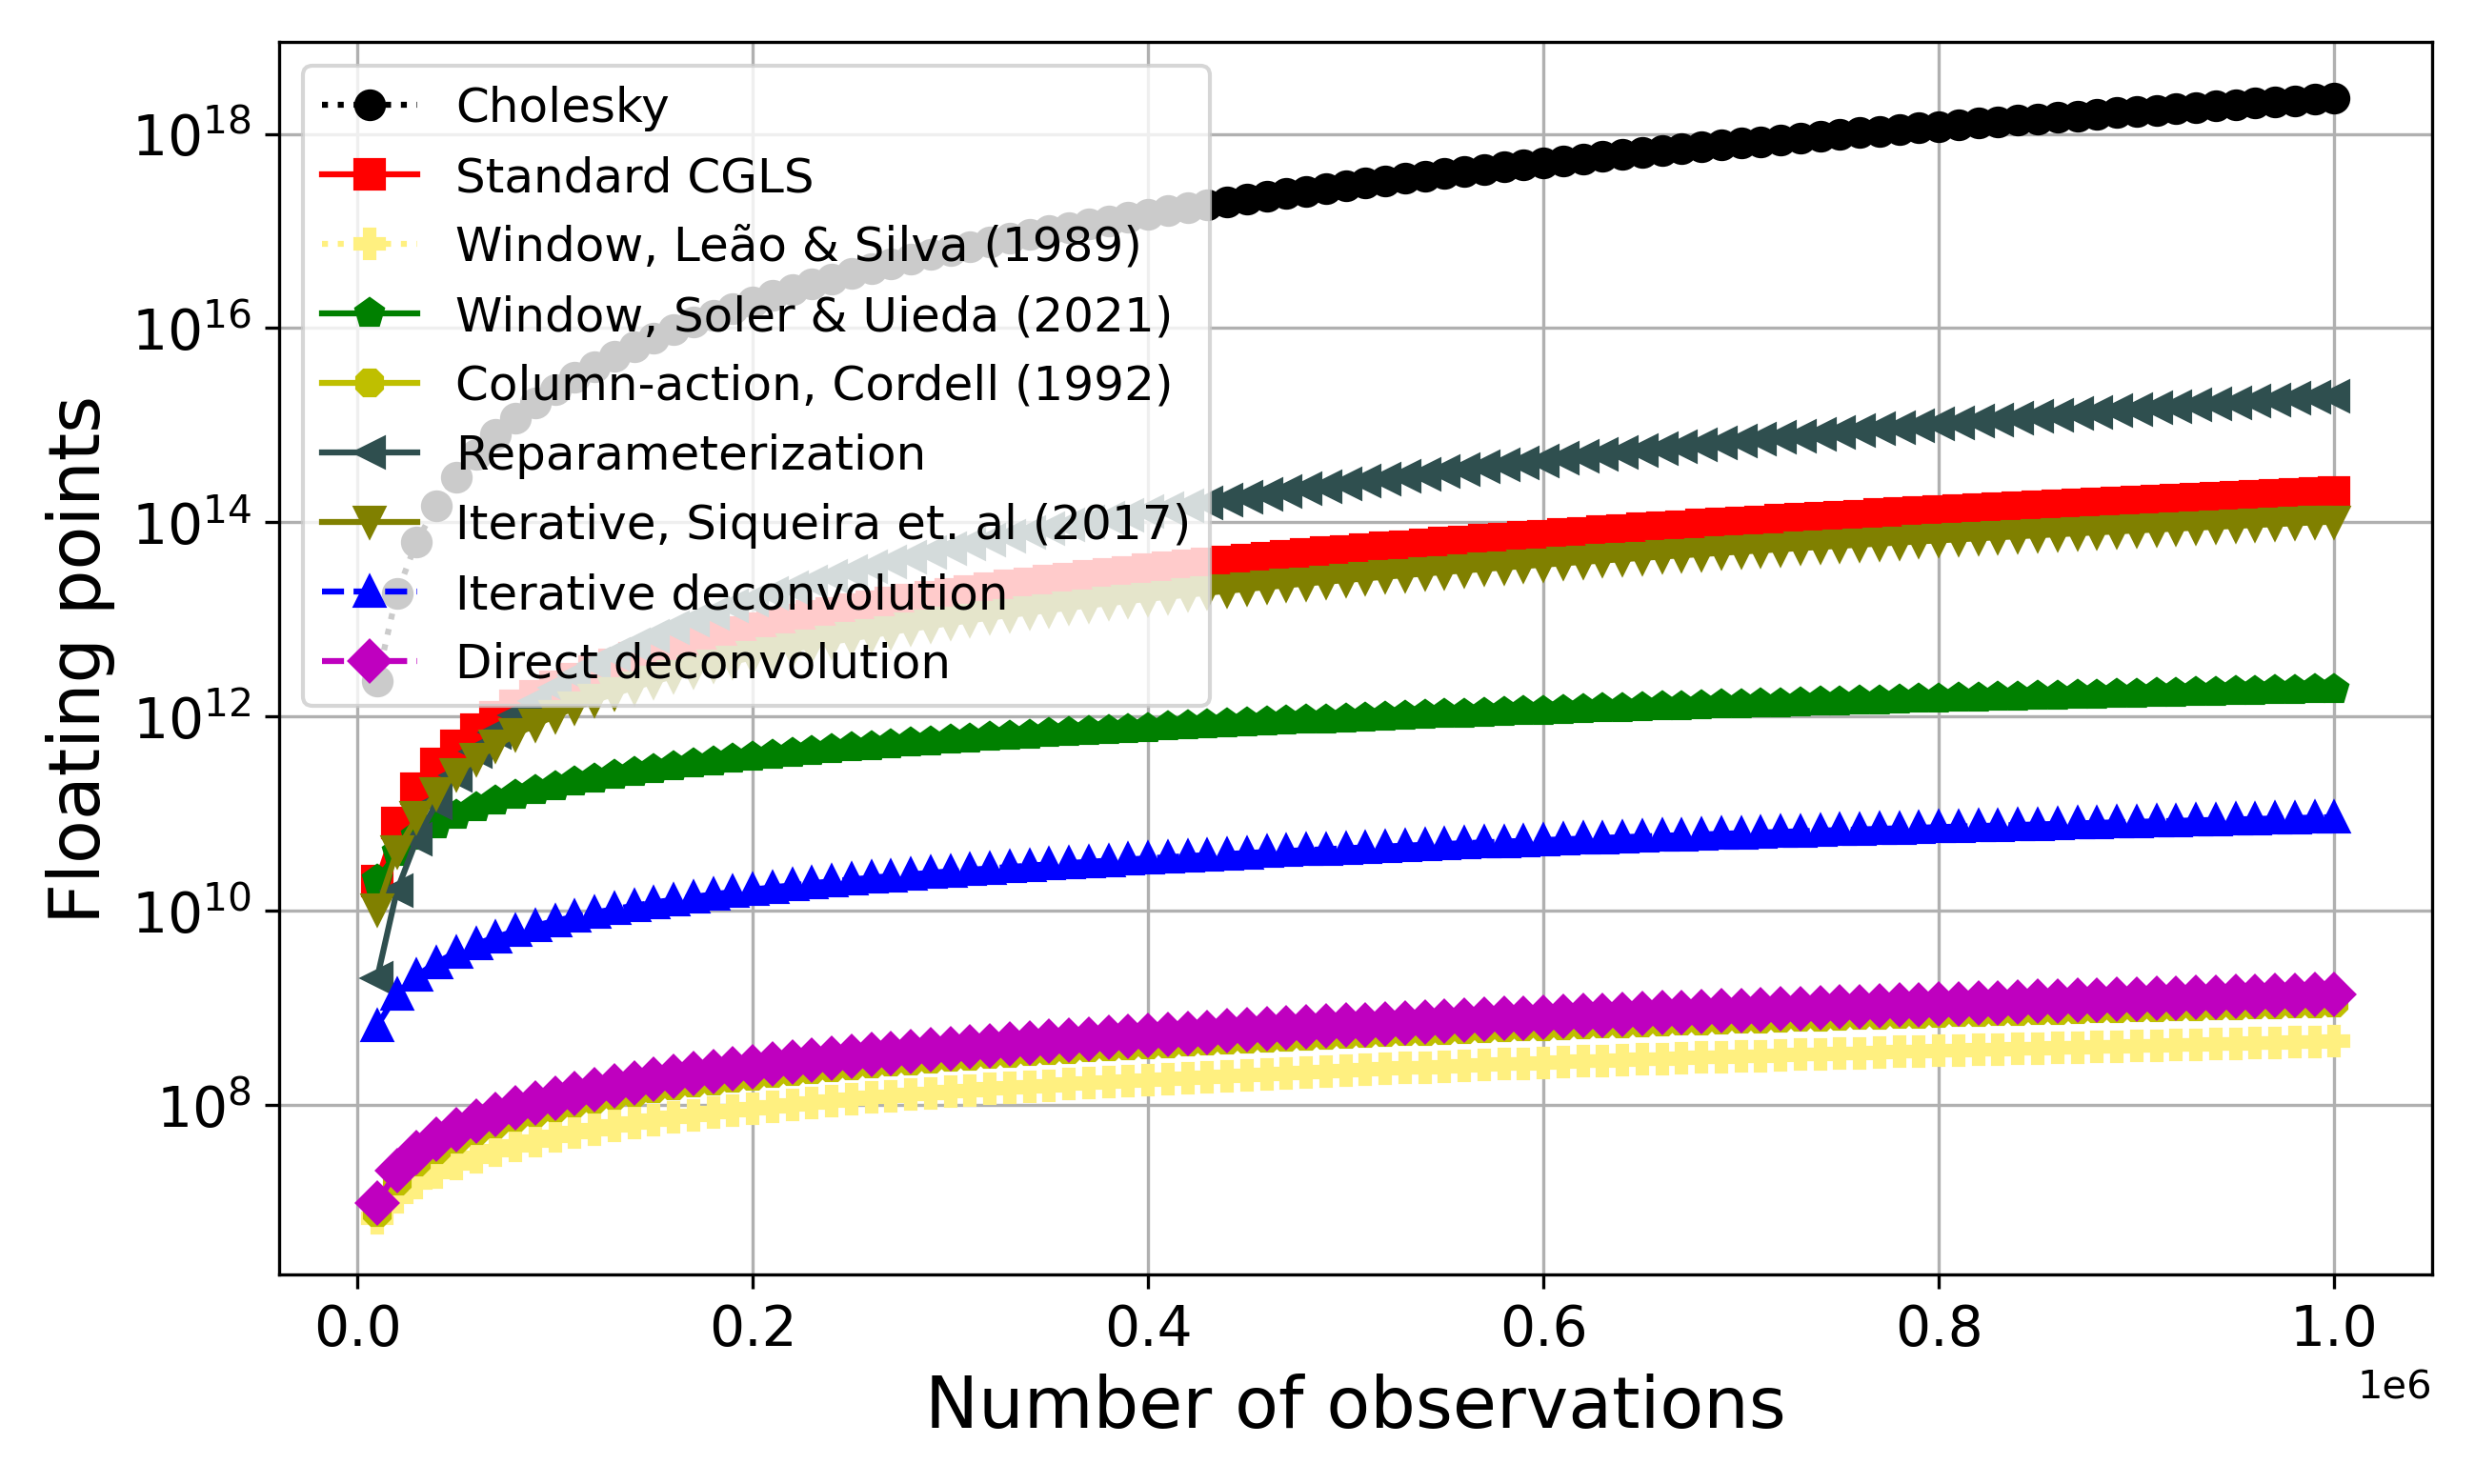
\includegraphics[width=9cm]{Fig/flops_grav}% This is a *.eps file
\end{center}
\caption{Number of \textit{flops} for many of the methods described in this work to estimate the equivalent sources using gravity data. The range of observations varies from $10,000$ to $1,000,000$.}
\label{fig:1}
\end{figure}

\begin{figure}[htbp]
	\begin{center}
		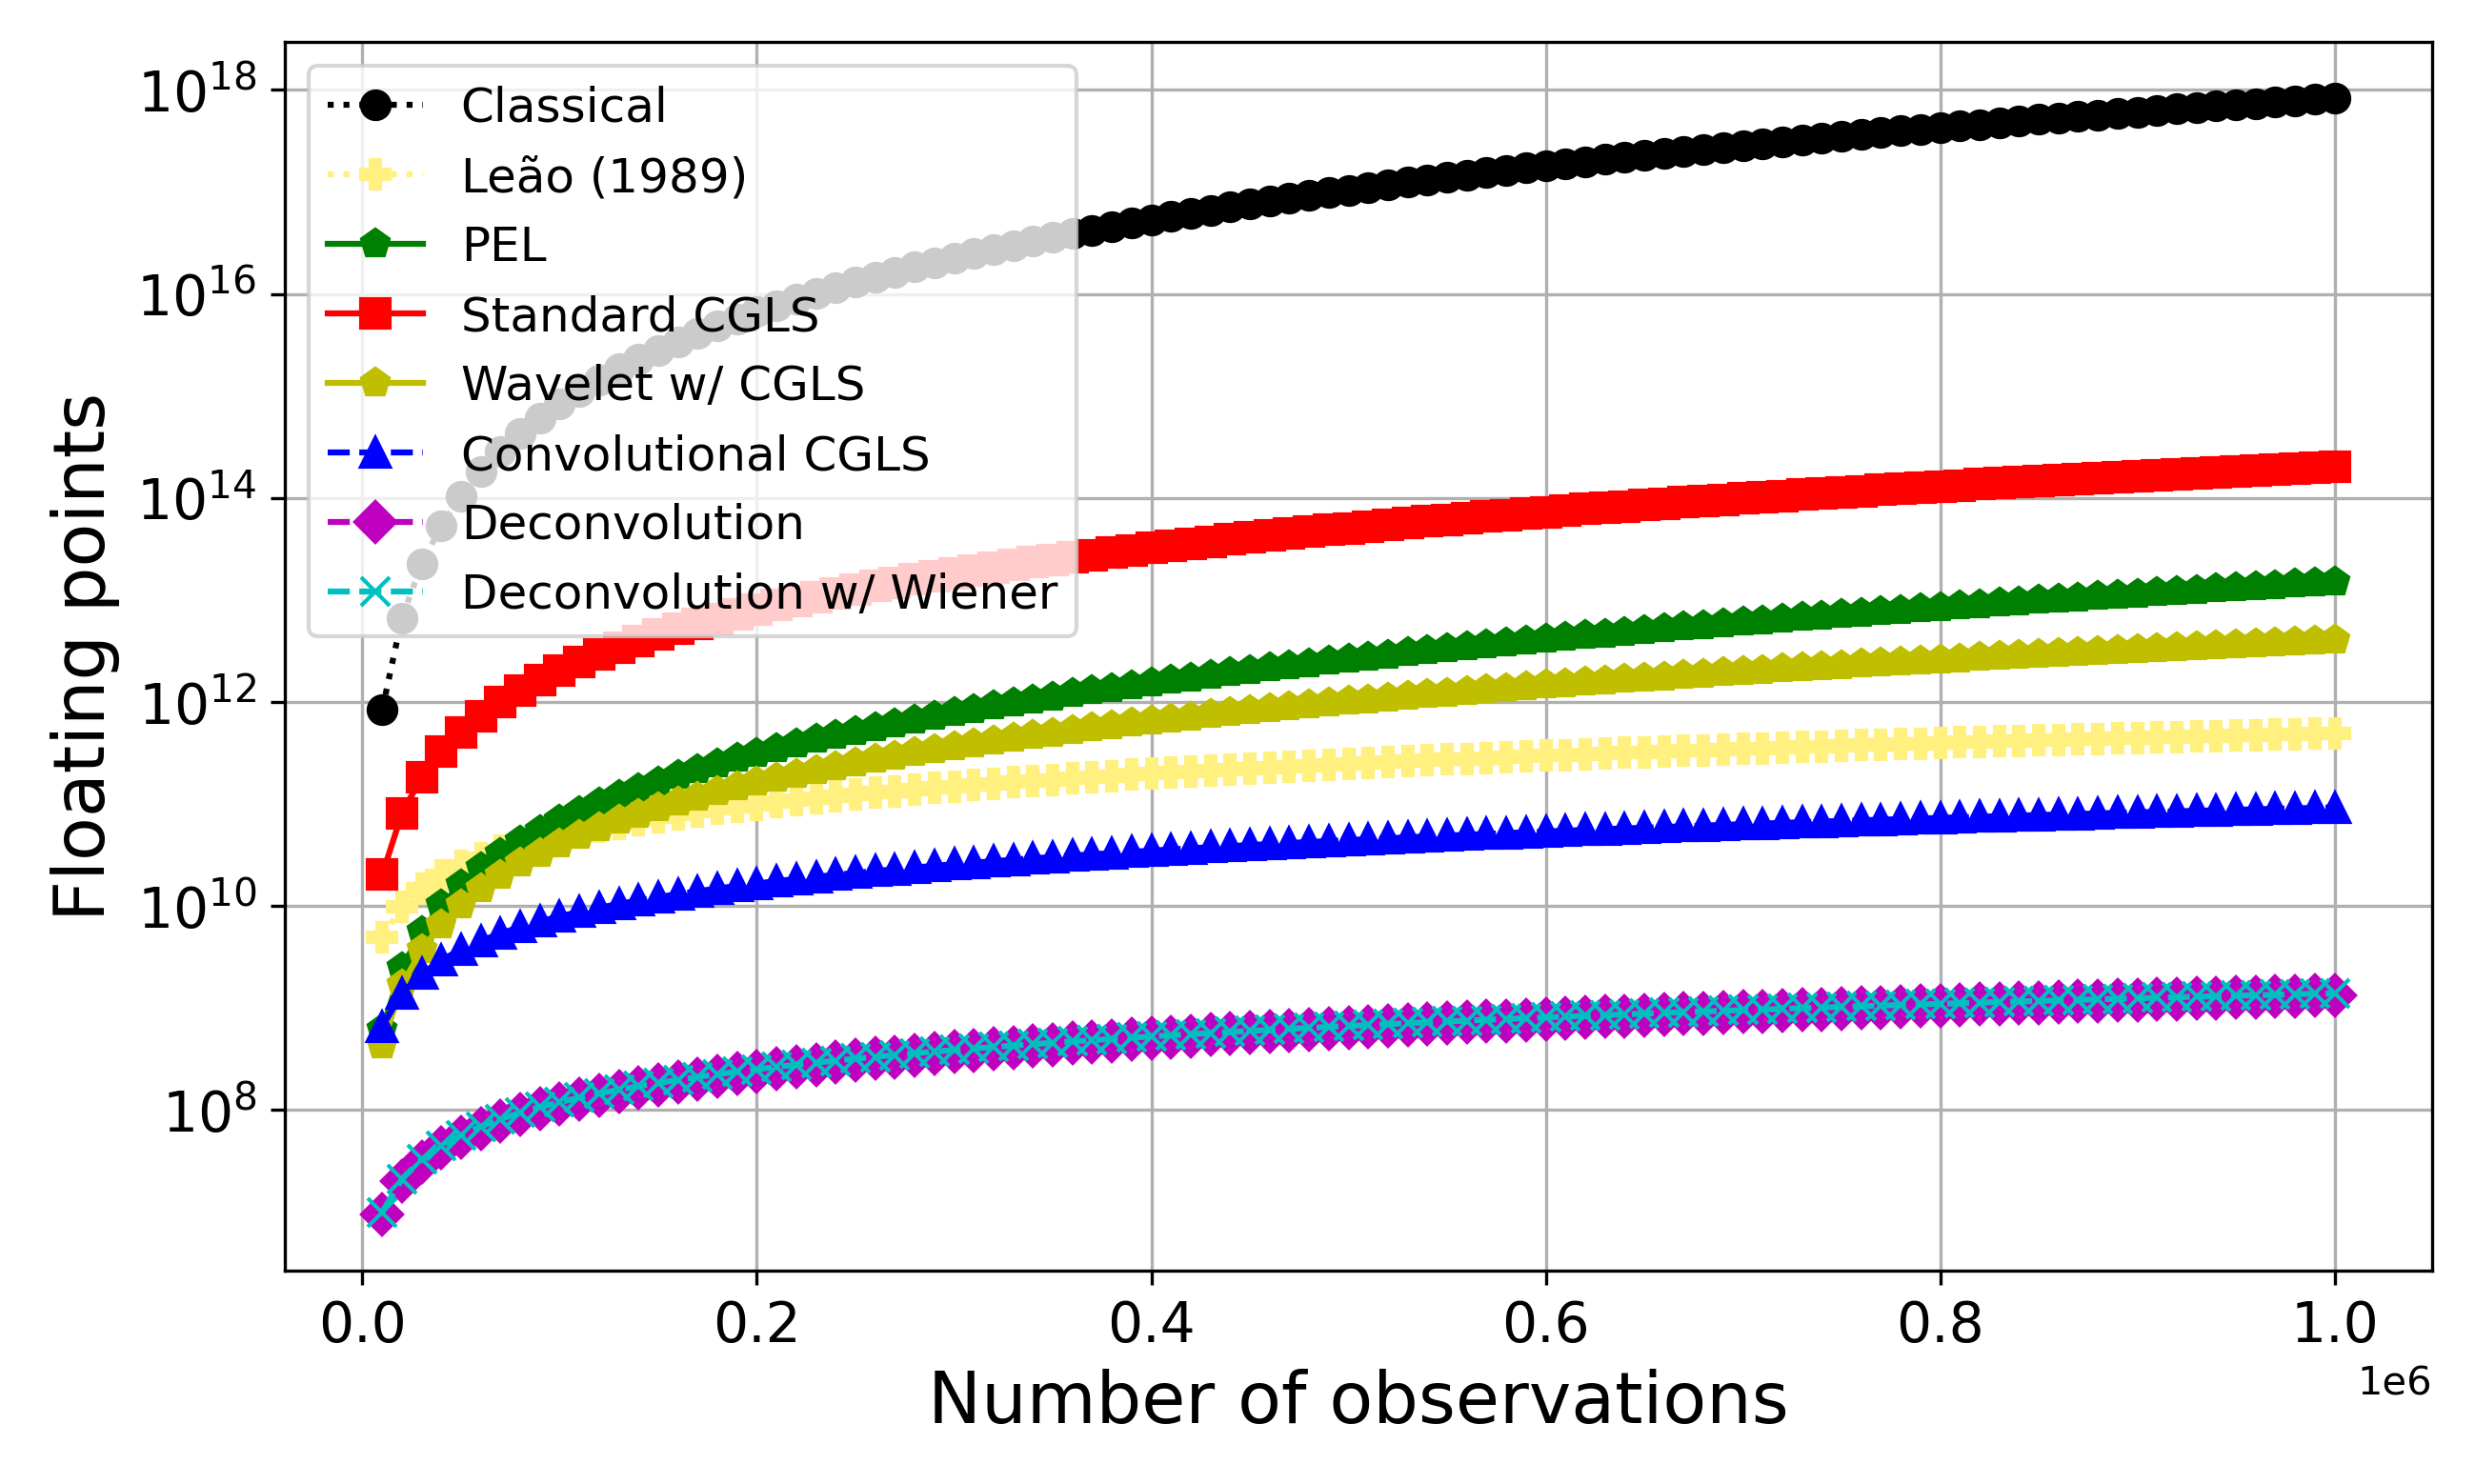
\includegraphics[width=9cm]{Fig/flops_mag}% This is a *.eps file
	\end{center}
	\caption{Number of \textit{flops} for many of the methods described in this work to estimate the equivalent sources using magnetic data. The range of observations varies from $10,000$ to $1,000,000$.}
	\label{fig:2}
\end{figure}

\begin{figure}[htbp]
	\begin{center}
		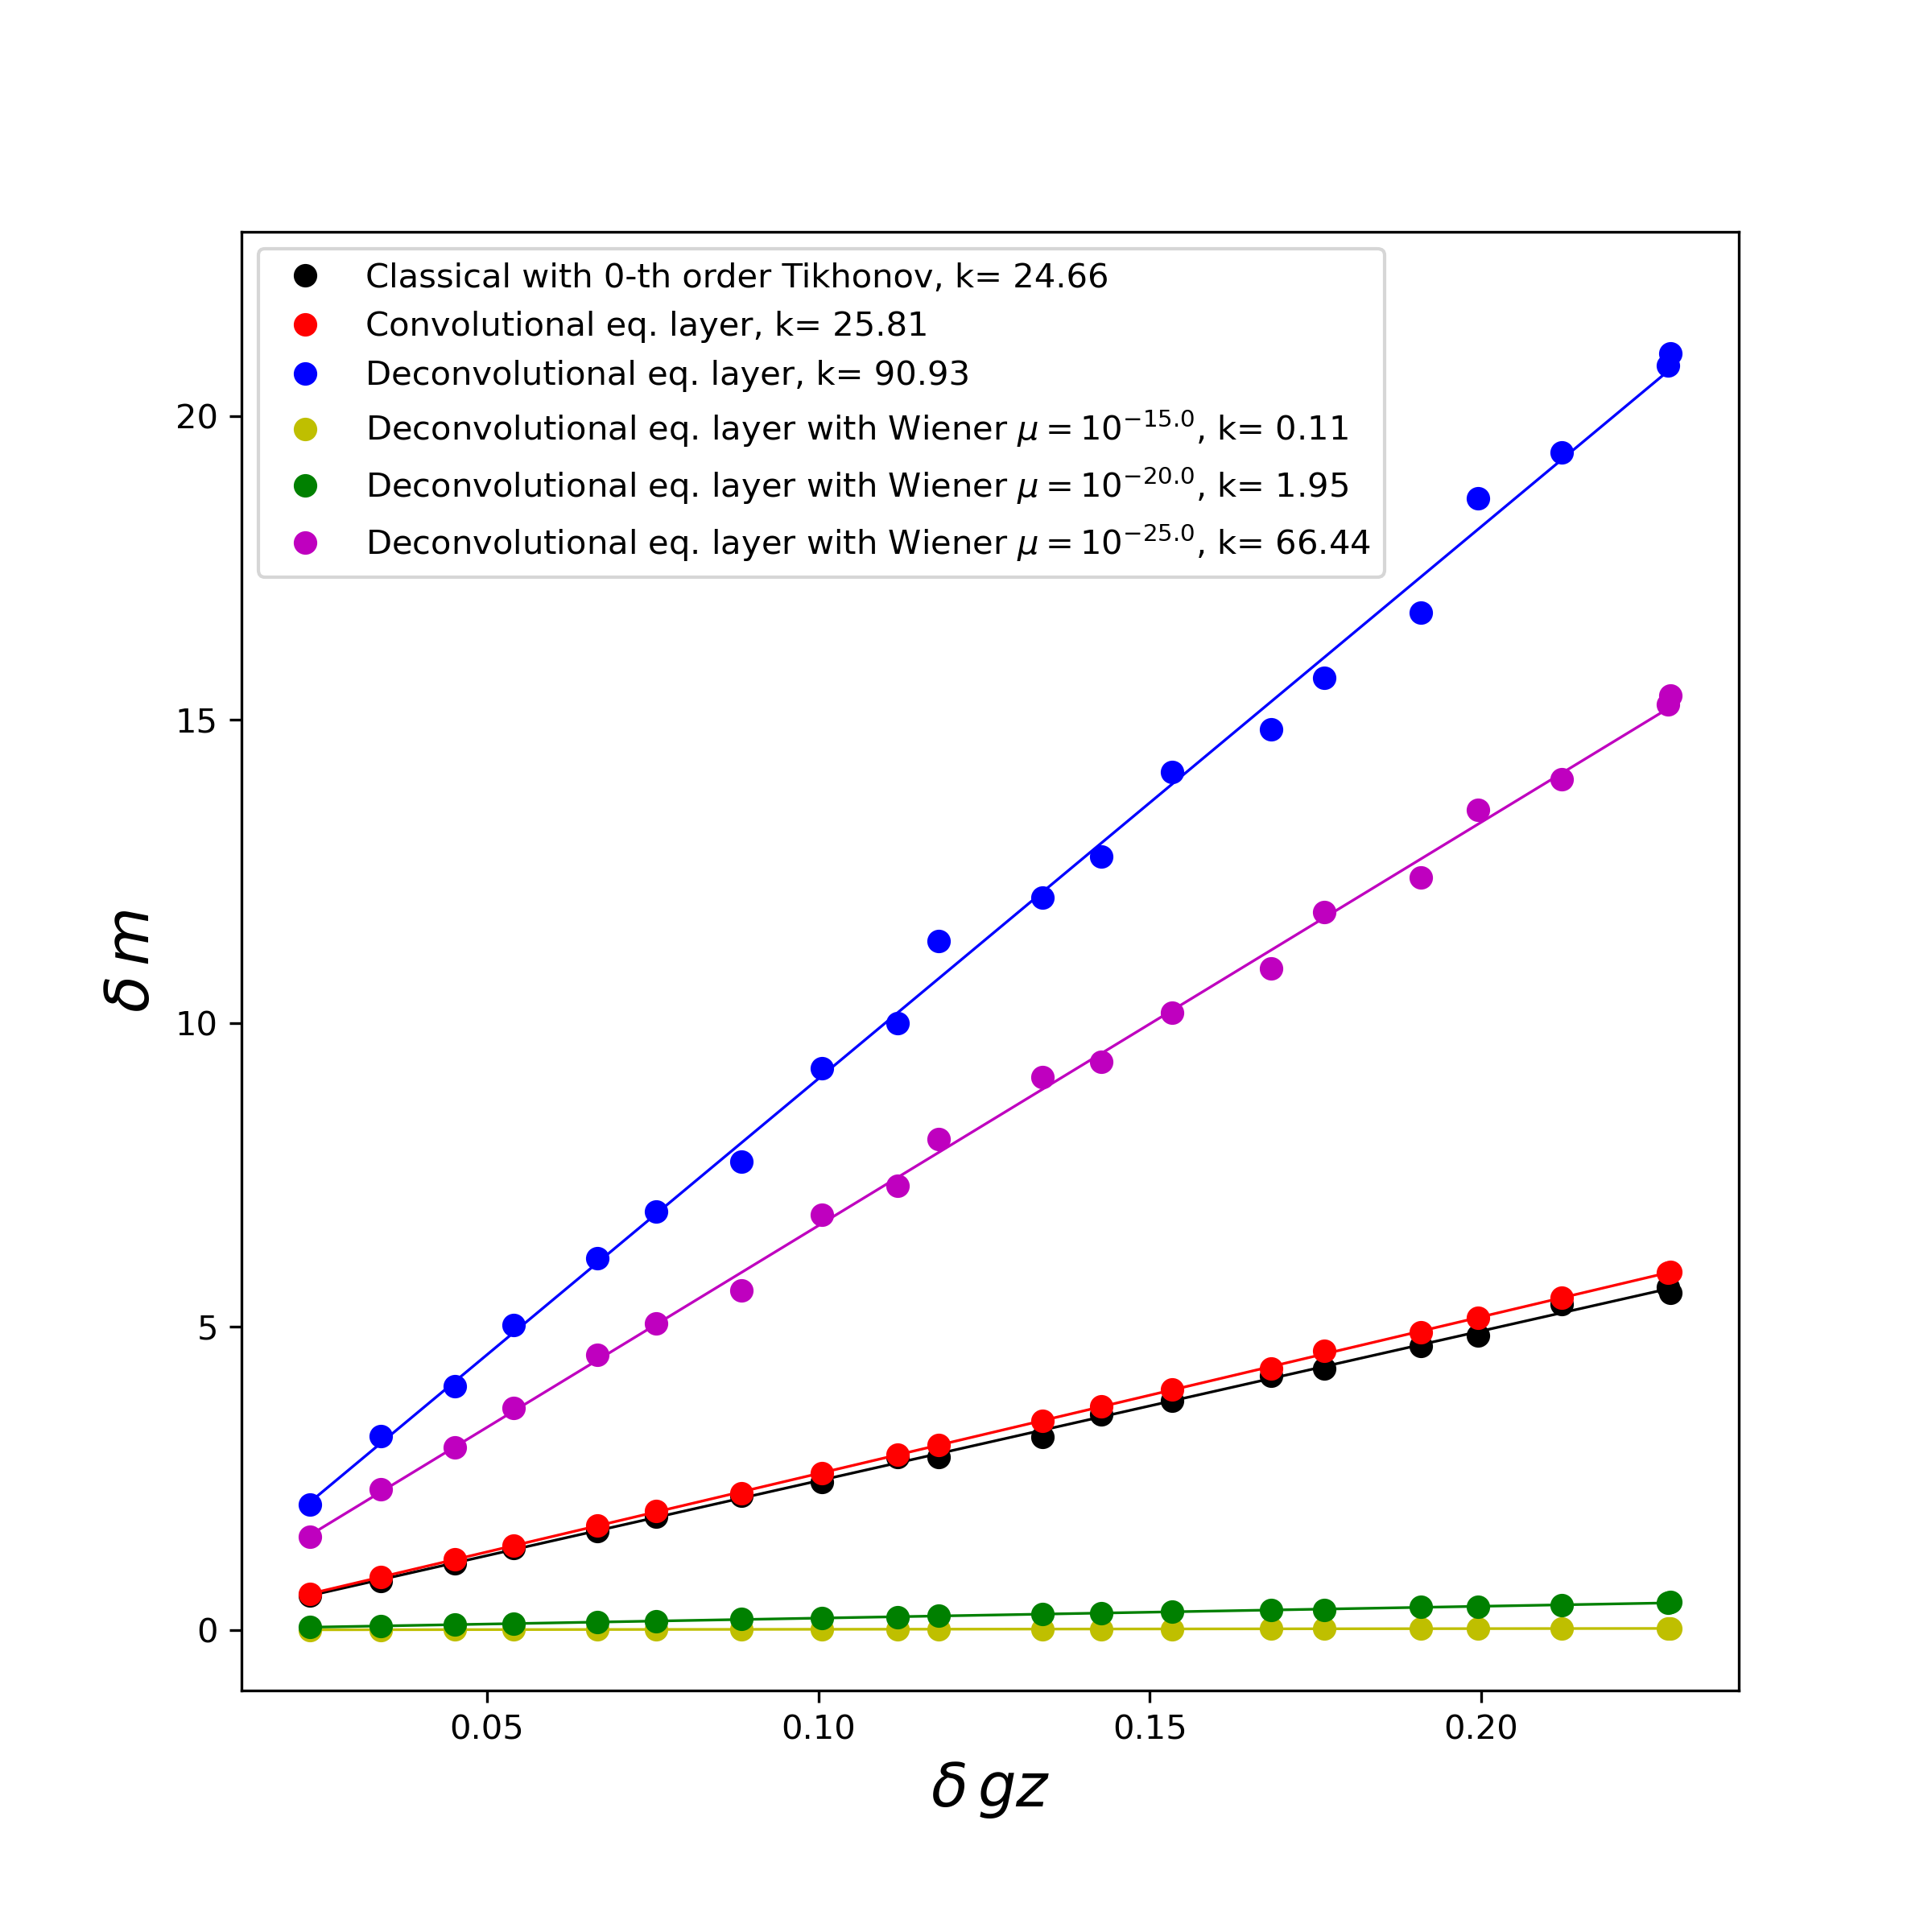
\includegraphics[width=9cm]{Fig/stability_grav}
	\end{center}
	\caption{Stability analysis of some of the equivalent layer methods of the gravimetric case.}
	\label{fig:3}
\end{figure}

\begin{figure}[htbp]
	\begin{center}
		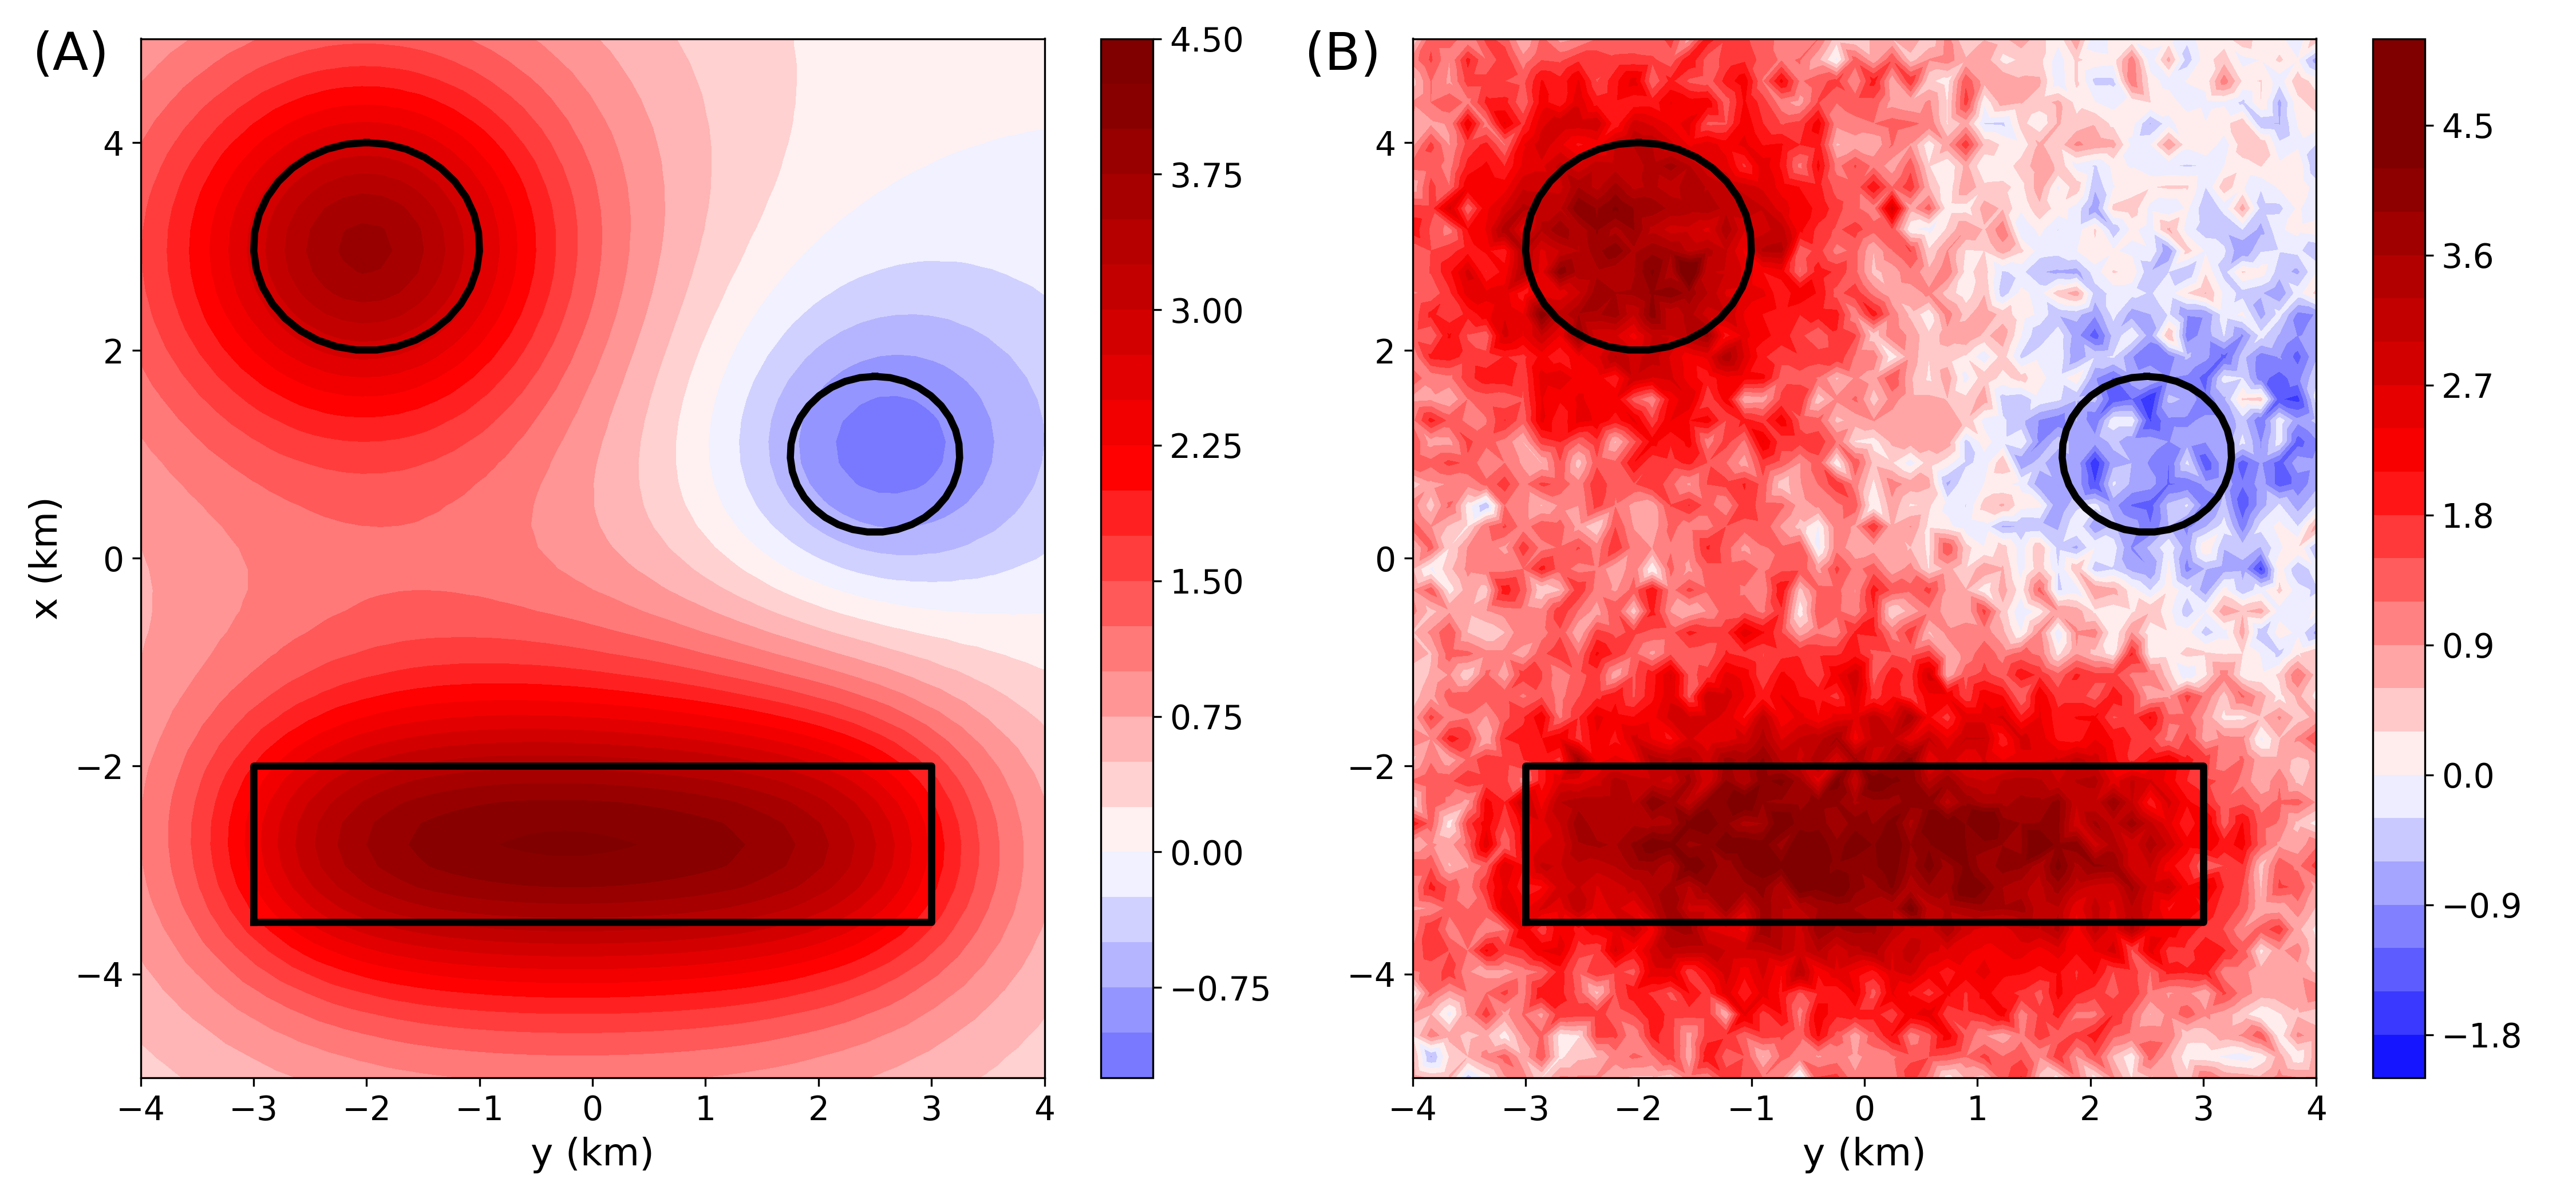
\includegraphics[width=9cm]{Fig/synthetic_grav}
	\end{center}
	\caption{Synthetic data of the gravimetric case. The observations points are placed in a regular grid of $50 \times 50$. Panel (A) shows the noise-free data and panel (B) shows the maximum noised data ($10\%$).}
	\label{fig:4}
\end{figure}

\begin{figure}[htbp]
	\begin{center}
		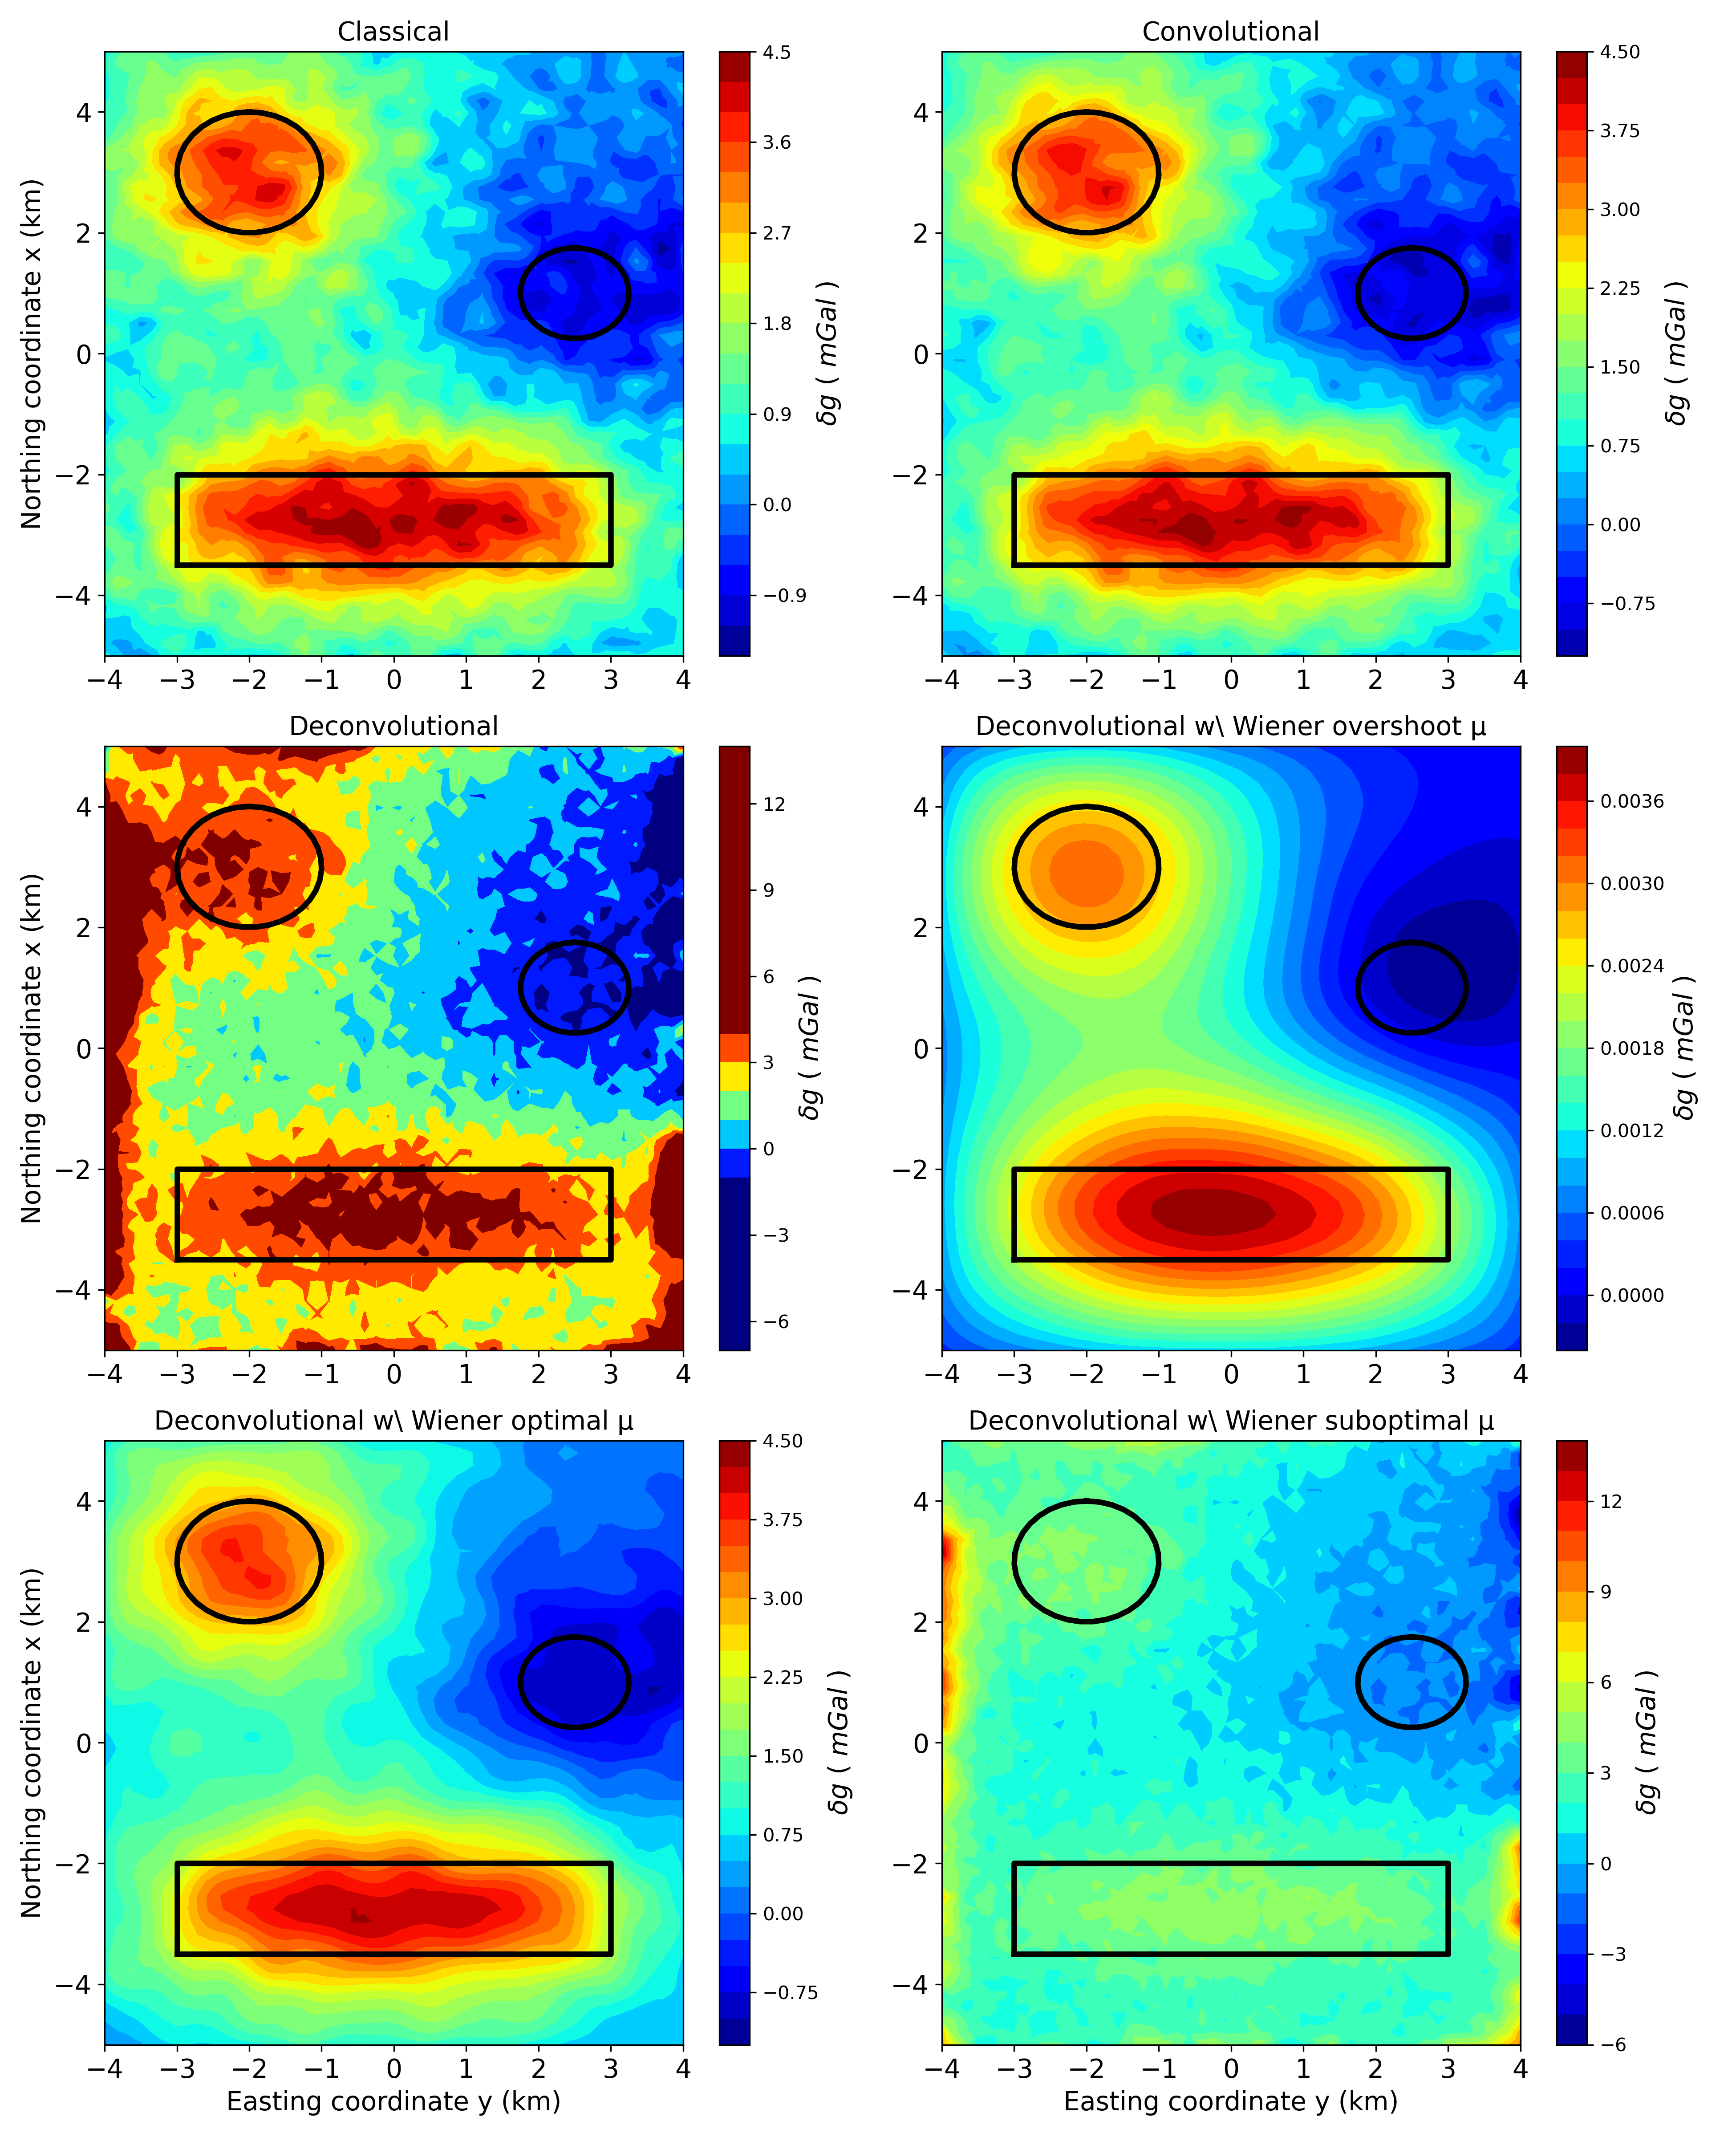
\includegraphics[width=10cm]{Fig/stability_grav_comparison}
	\end{center}
	\caption{Predicted gravity data for different methods of the equivalent layer with maximum level of noise. Panel \textbf{(A)} is the classical method, \textbf{(B)} is the convolutional, \textbf{(C)} is the deconvolutional, \textbf{(D)} is the deconvolutional method using Wiener stabilization with a too high value for $\mu$, \textbf{(E)} is the deconvolutional method using Wiener stabilization with a optimal value for $\mu$ and \textbf{(F)} is the deconvolutional method using Wiener stabilization with a too low value for $\mu$.}
	\label{fig:5}
\end{figure}

\begin{figure}[htbp]
	\begin{center}
		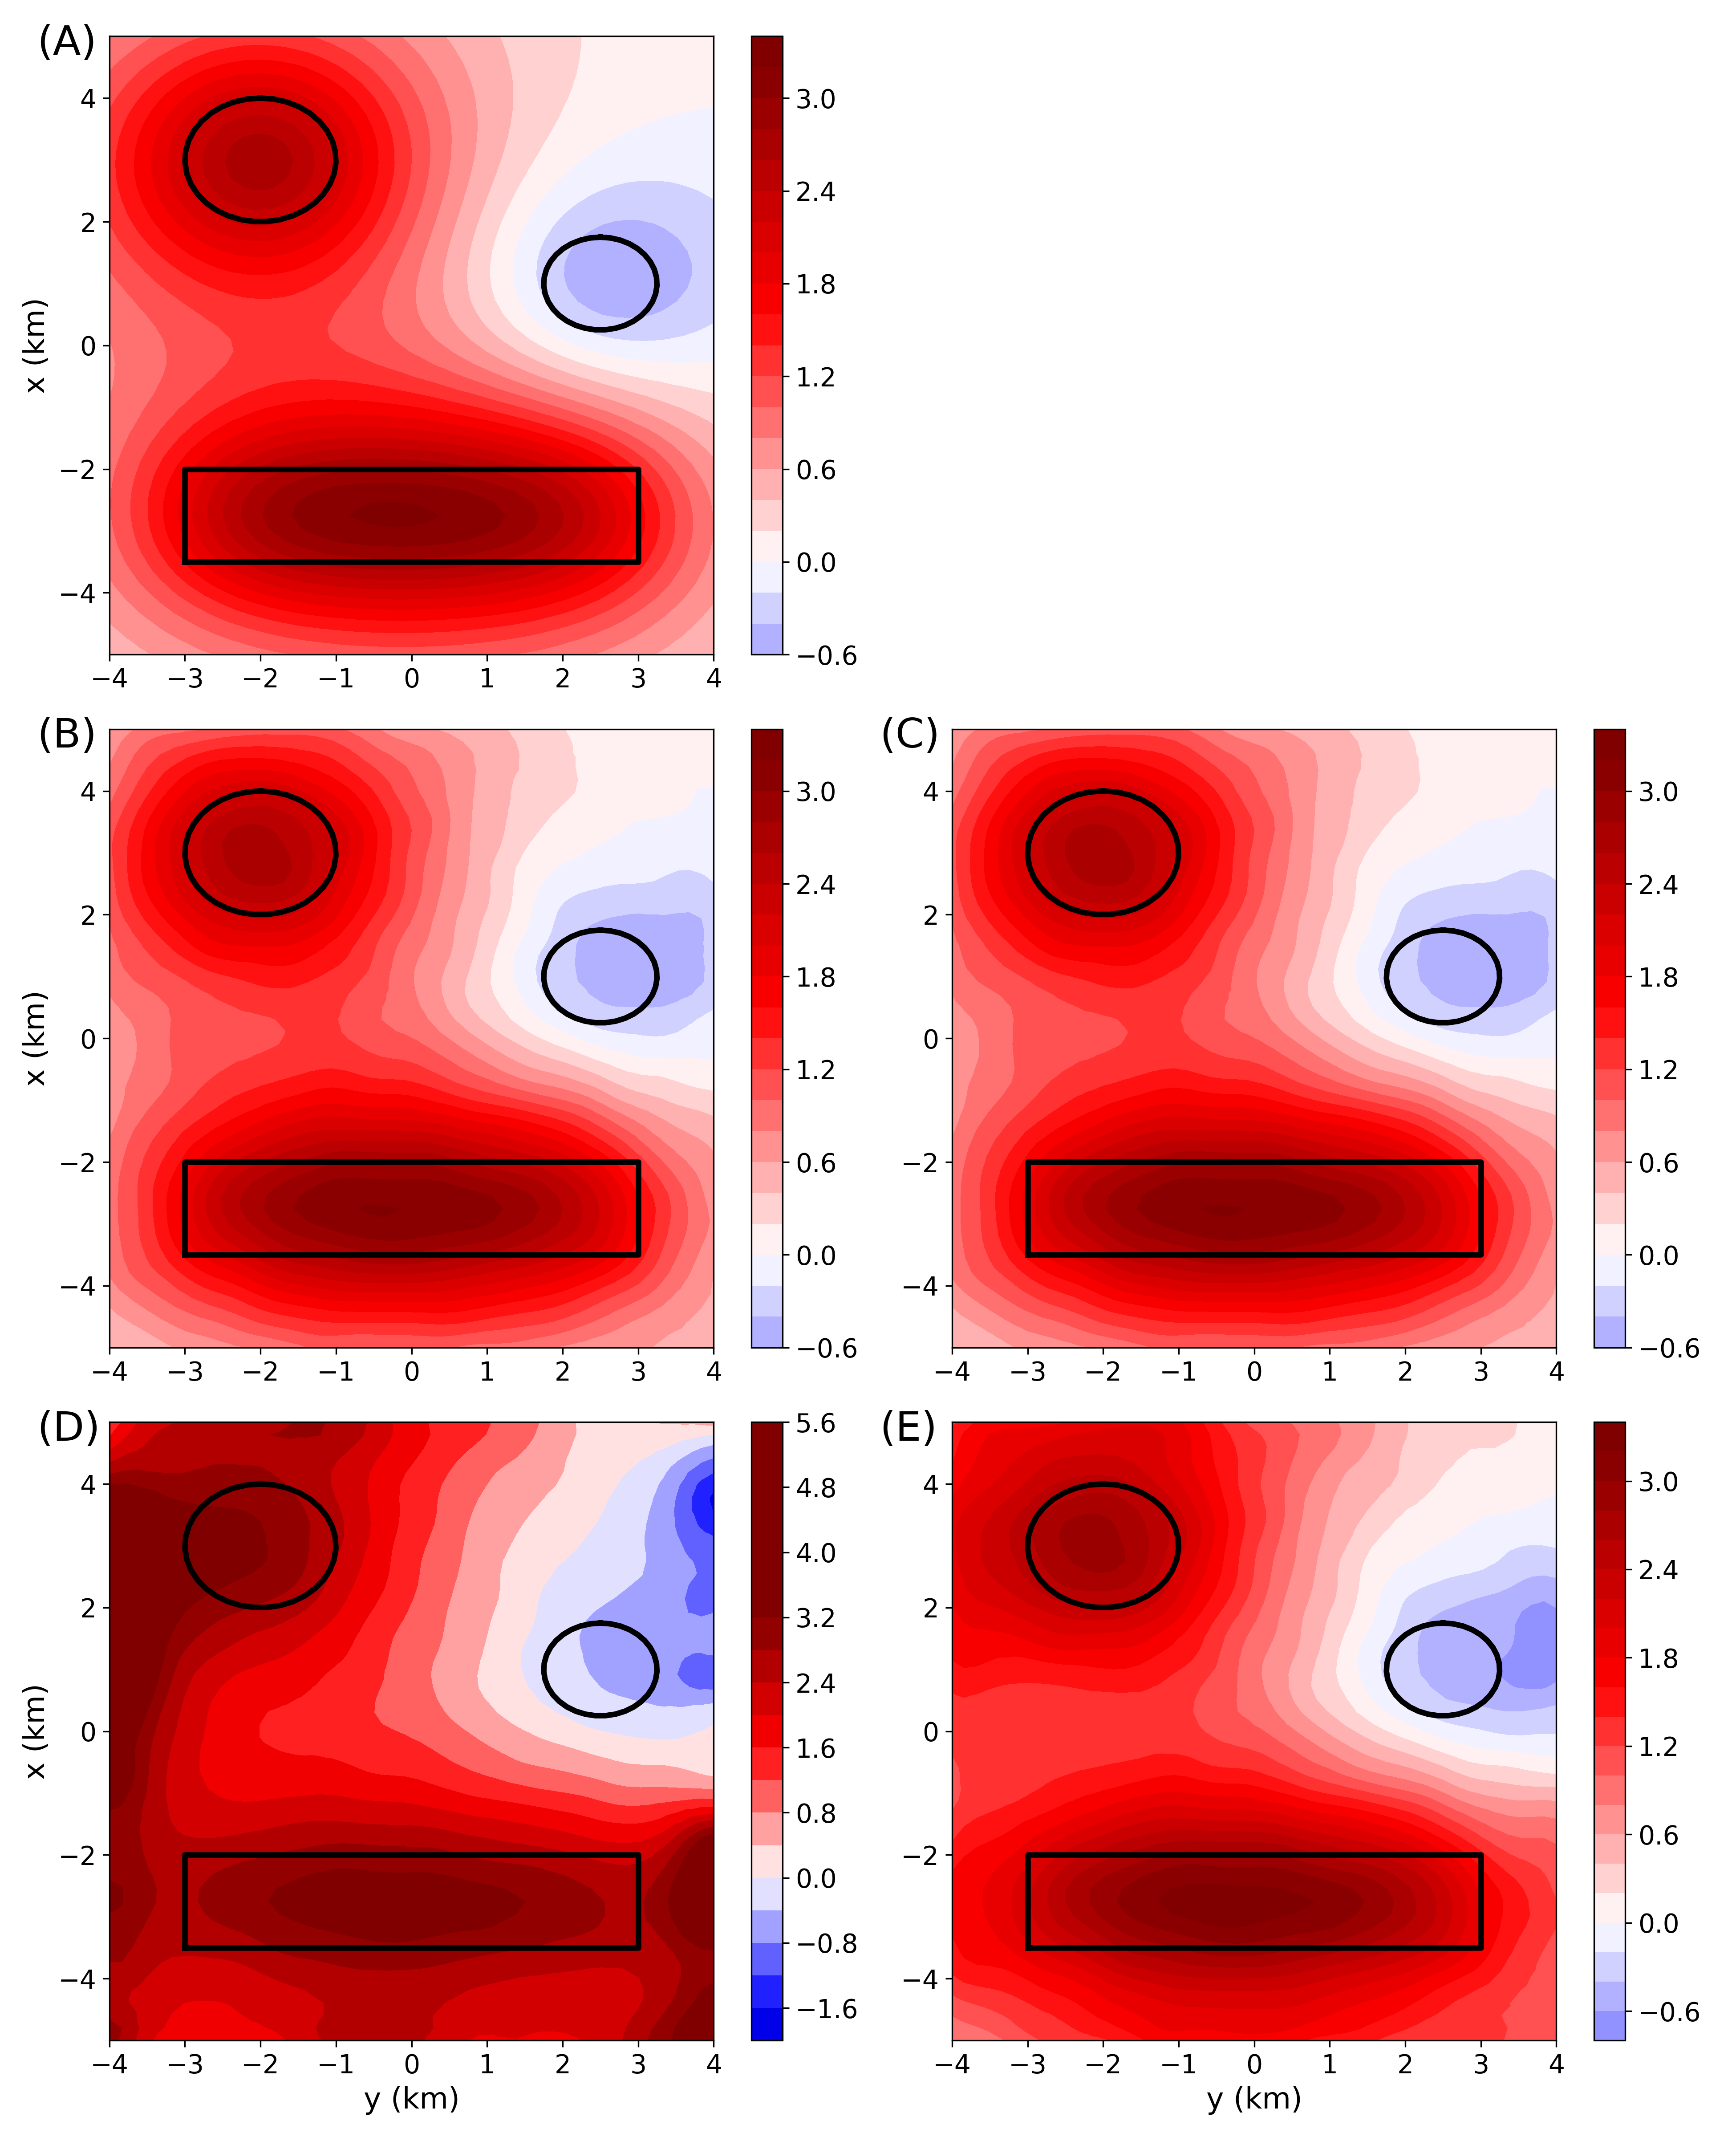
\includegraphics[width=10cm]{Fig/grav_upward}
	\end{center}
	\caption{True noiseless upward gravimetric data at $z_i = -500$ m height and predicted data for different methods of the equivalent layer with maximum level of noise. Panel \textbf{(A)} is the true upward gravity data, Panel \textbf{(B)} is the classical method, \textbf{(C)} is the convolutional, \textbf{(D)} is the deconvolutional, \textbf{(E)} is the deconvolutional method using Wiener stabilization with a optimal value for $\mu = 10^{-20}$.}
	\label{fig:grav_up}
\end{figure}

\begin{figure}[htbp]
	\begin{center}
		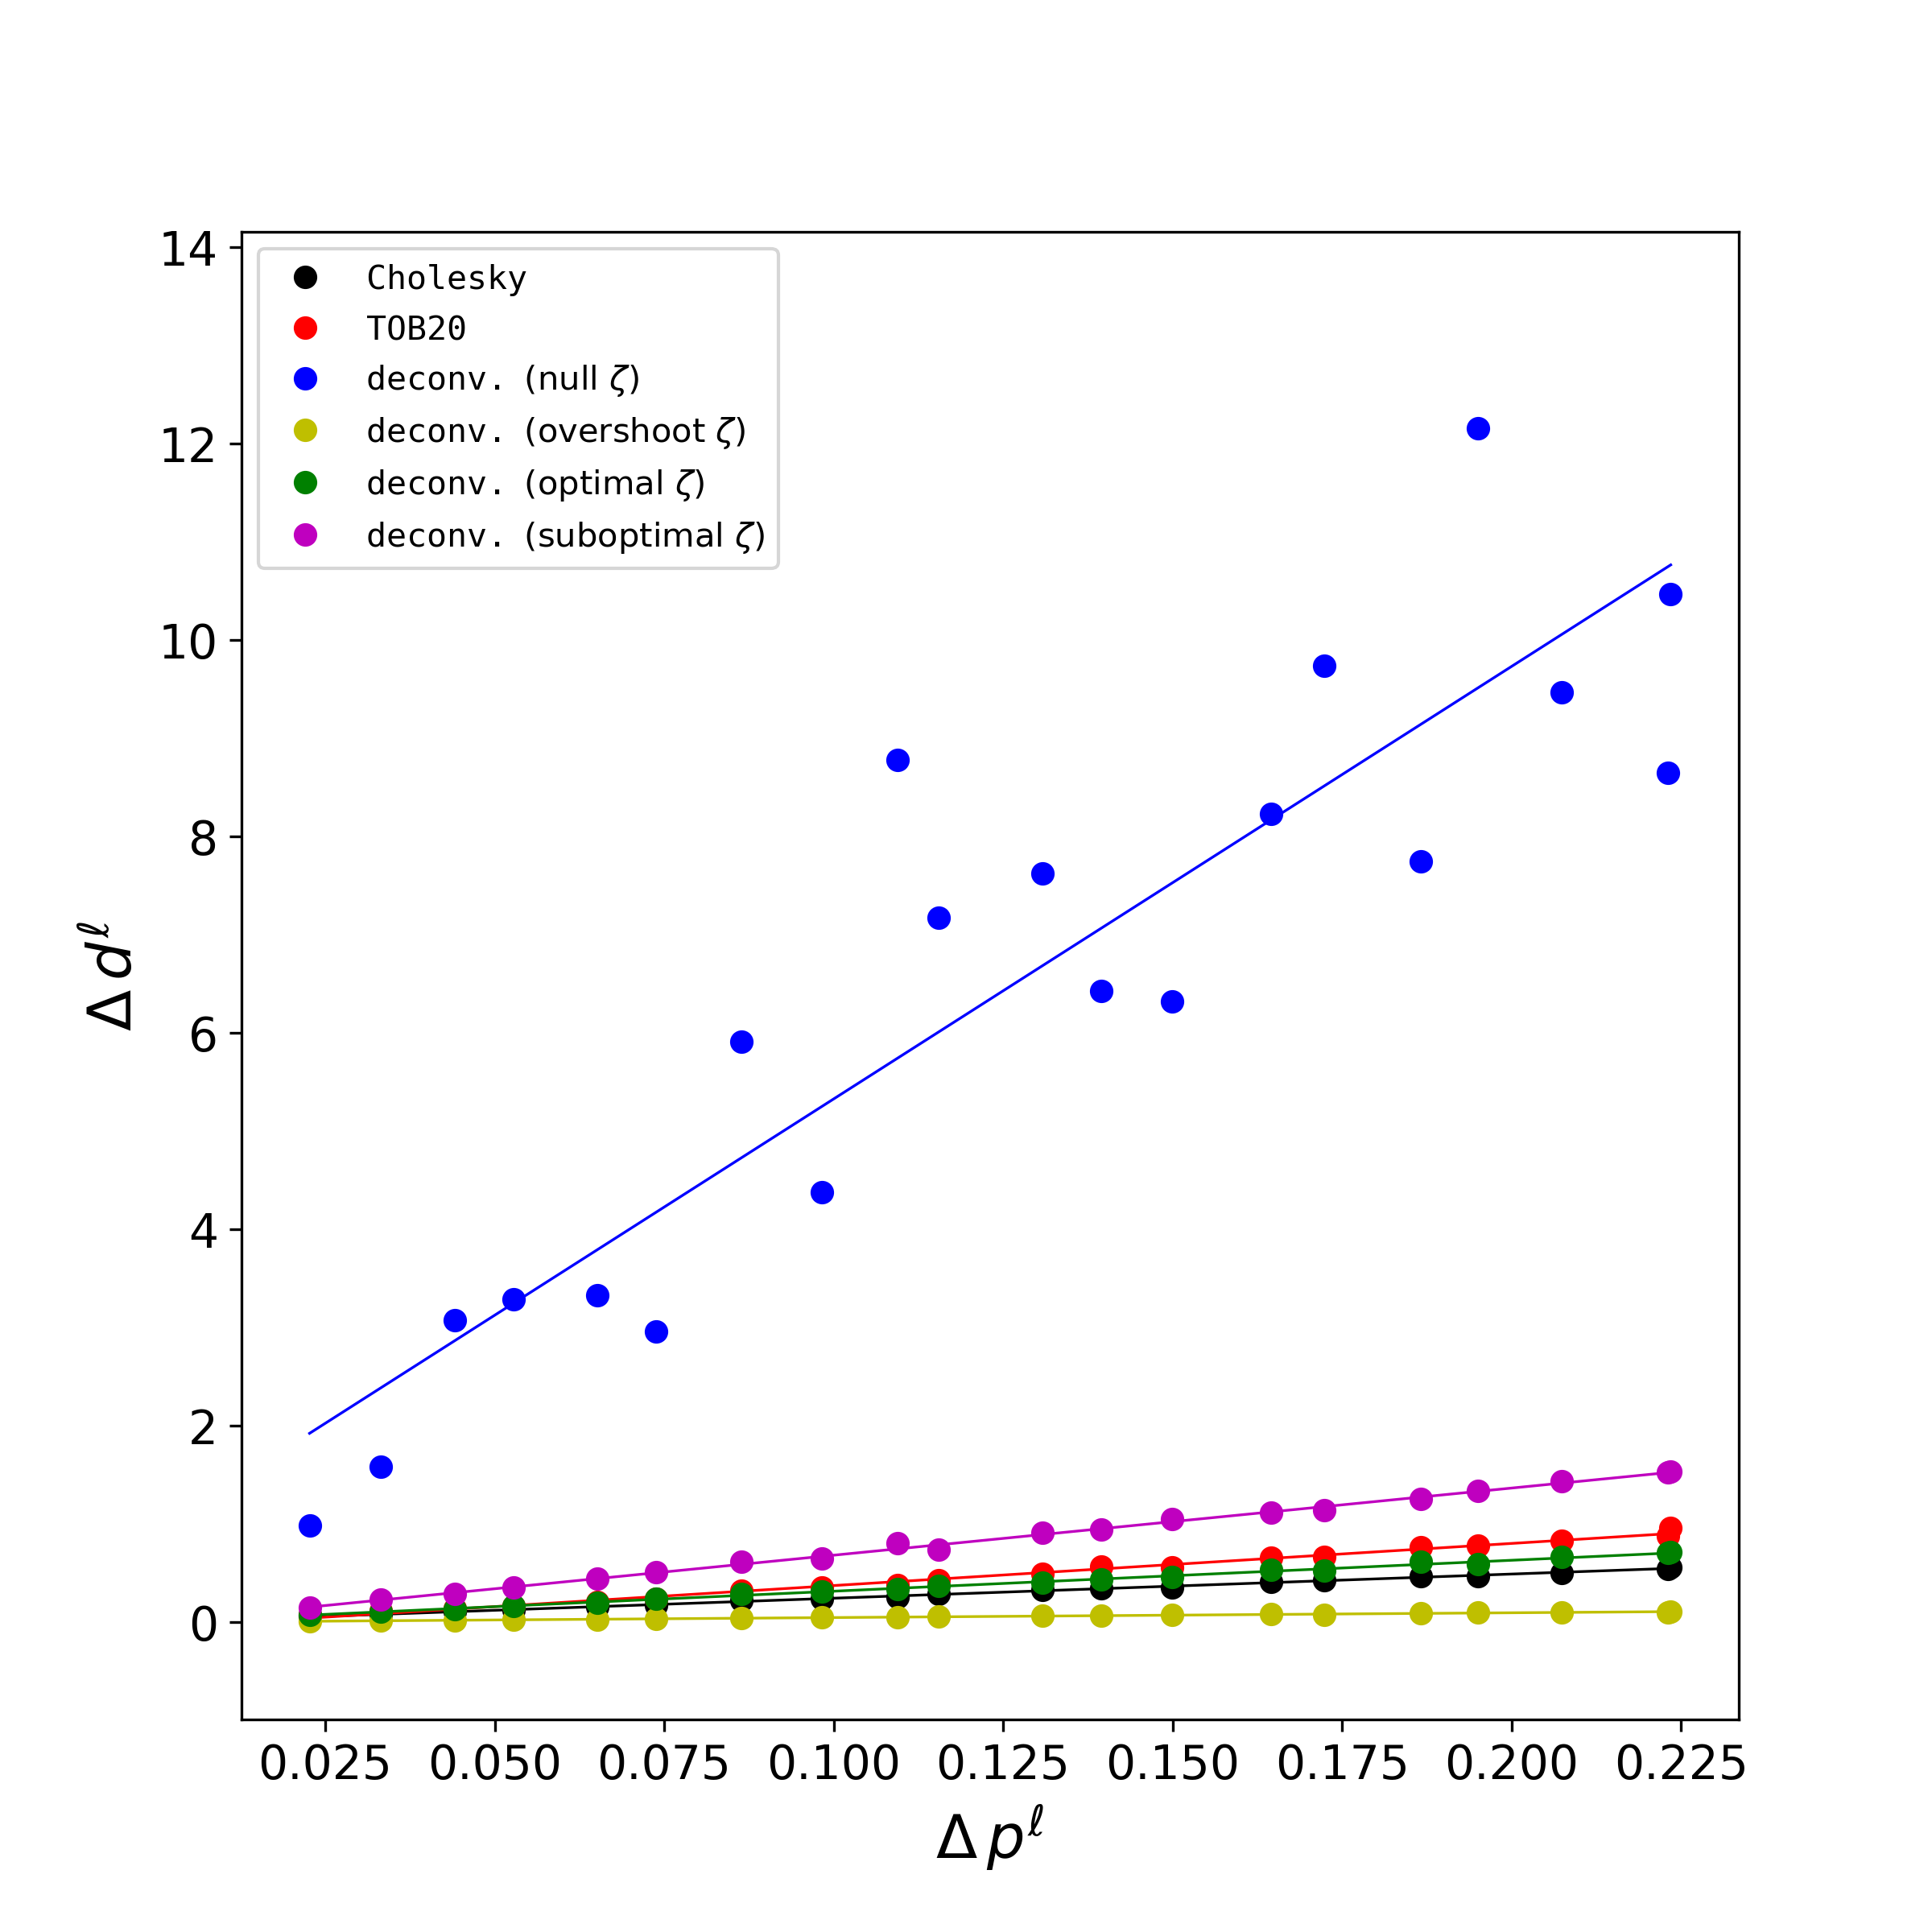
\includegraphics[width=10cm]{Fig/stability_mag}
	\end{center}
	\caption{Stability analysis of some of the equivalent layer methods of the magnetic case.}
	\label{fig:6}
\end{figure}

\begin{figure}[htbp]
	\begin{center}
		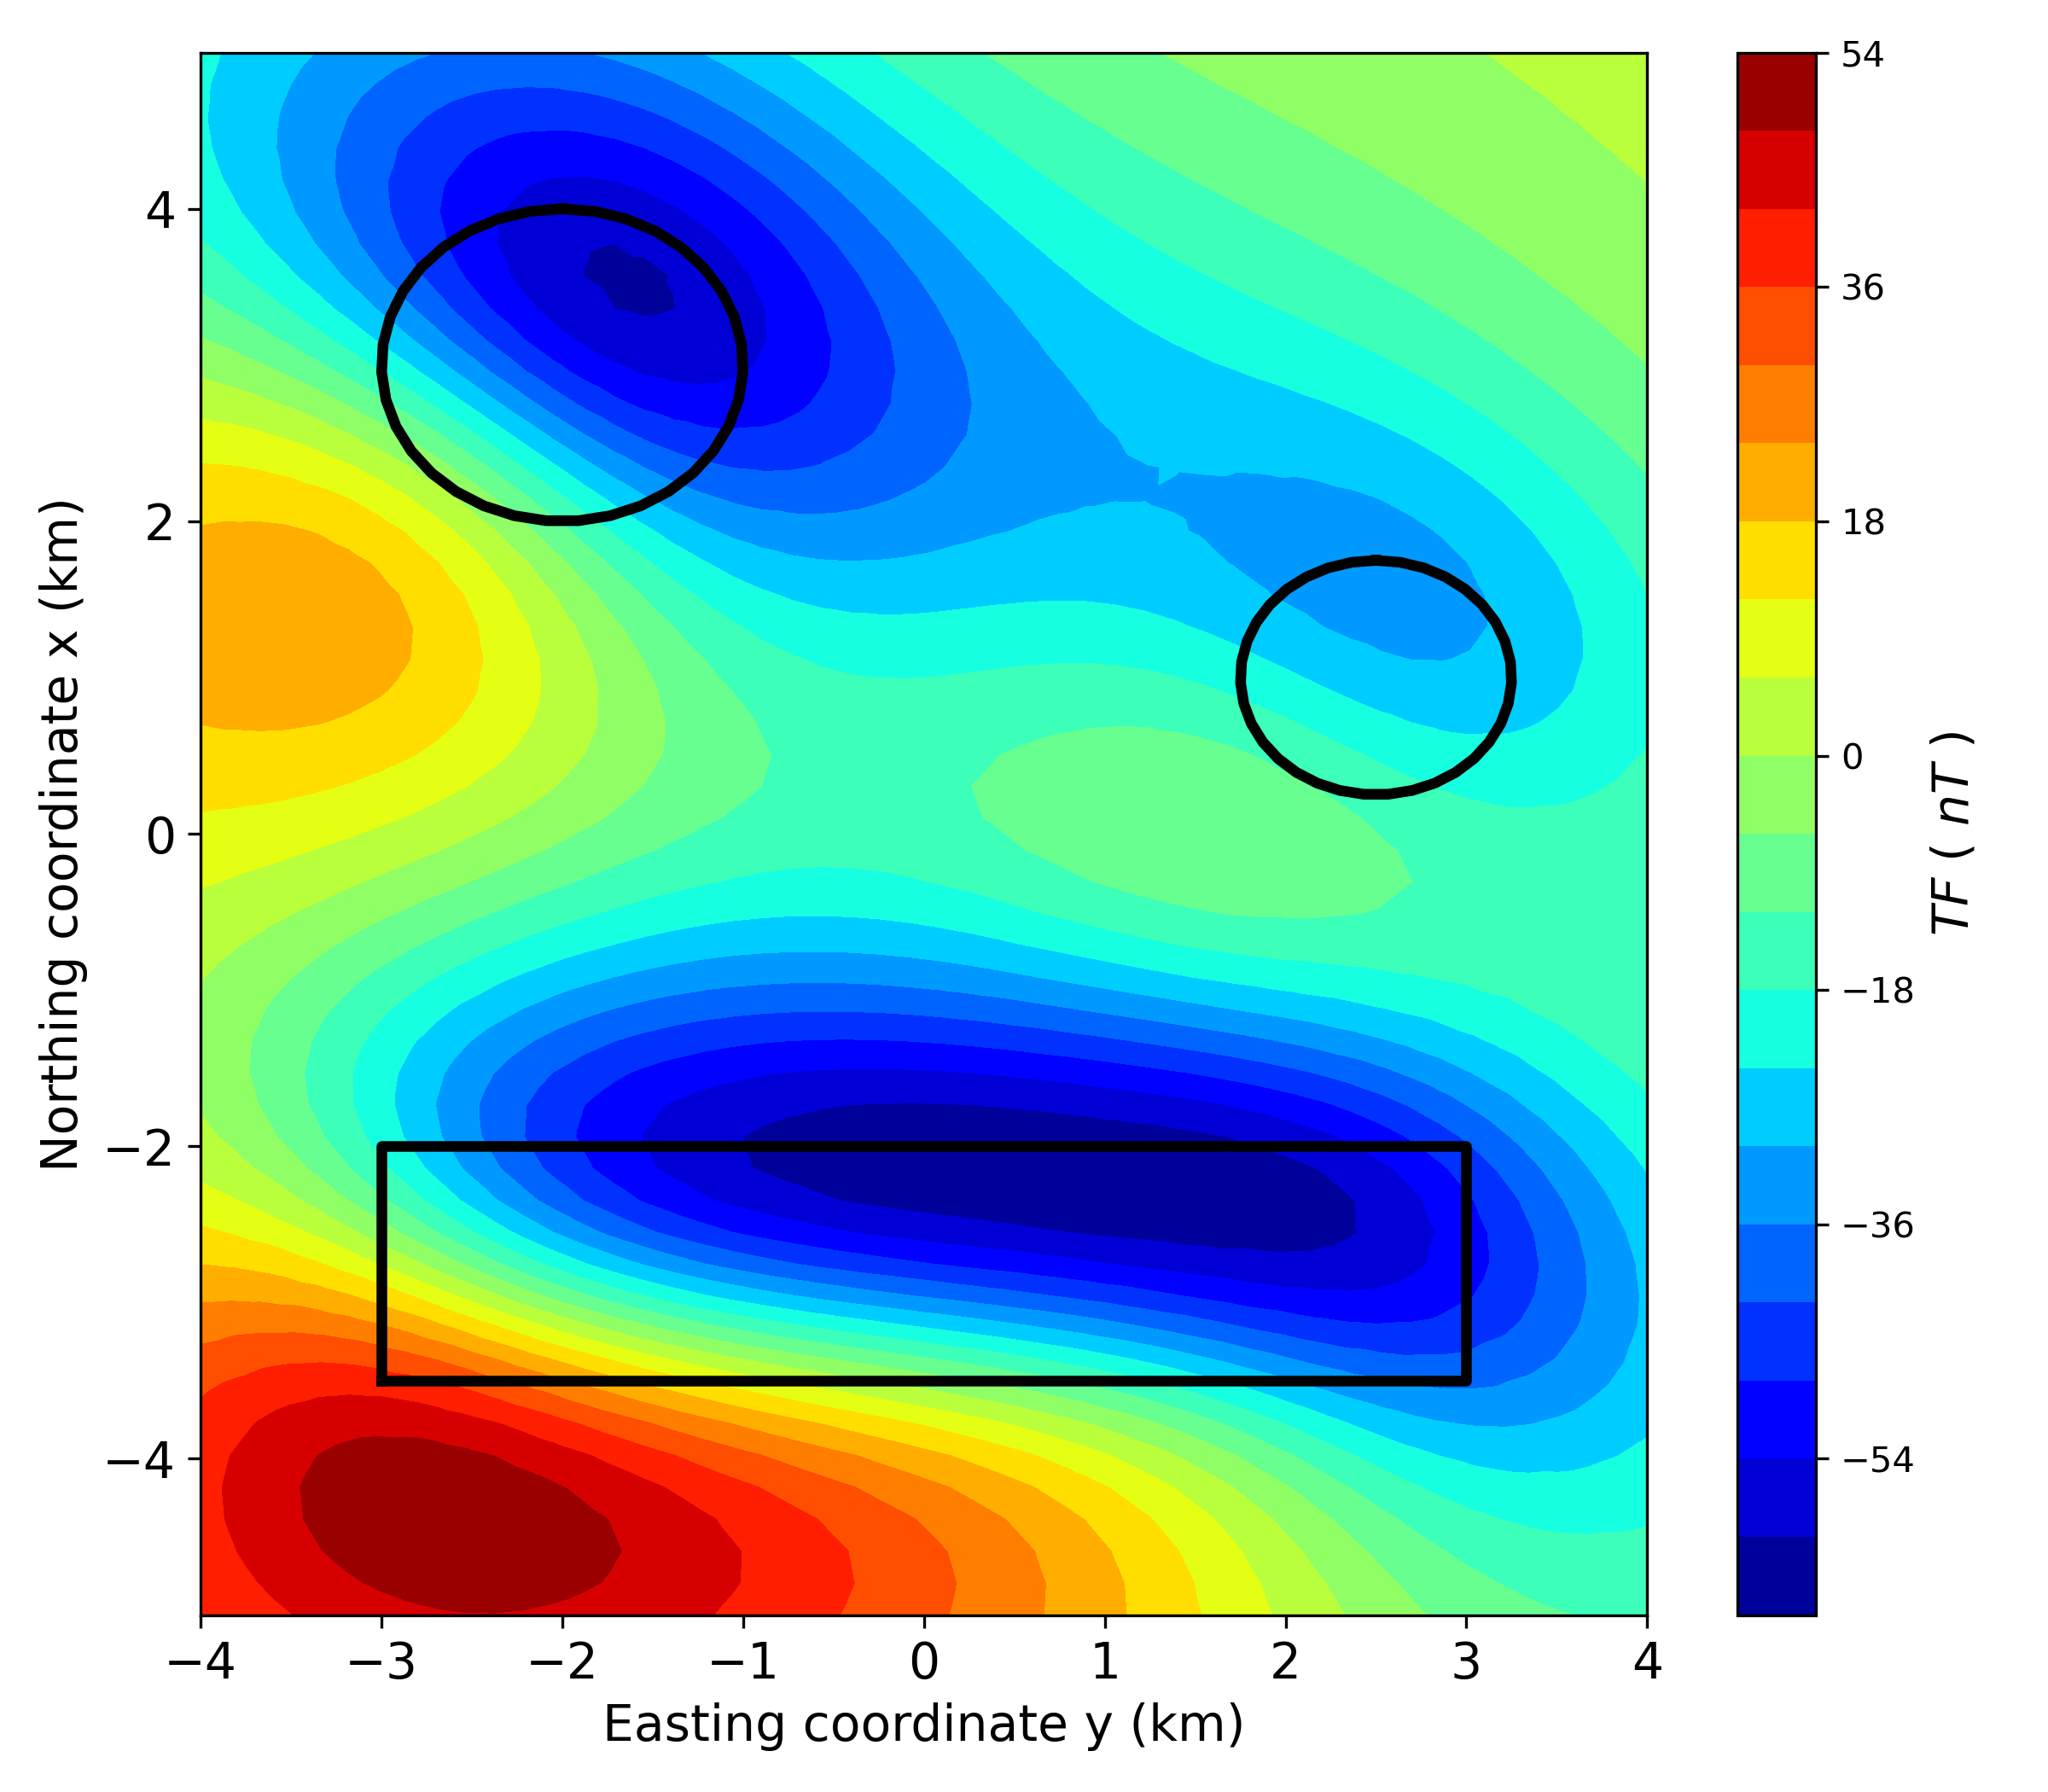
\includegraphics[width=10cm]{Fig/synthetic_mag}
	\end{center}
	\caption{Synthetic data of the magnetic case. The observations points are placed in a regular grid of $50 \times 50$. Panel (A) shows the noise-free data and panel (B) shows the maximum noised data ($10\%$).}
	\label{fig:7}
\end{figure}

\begin{figure}[htbp]
	\begin{center}
		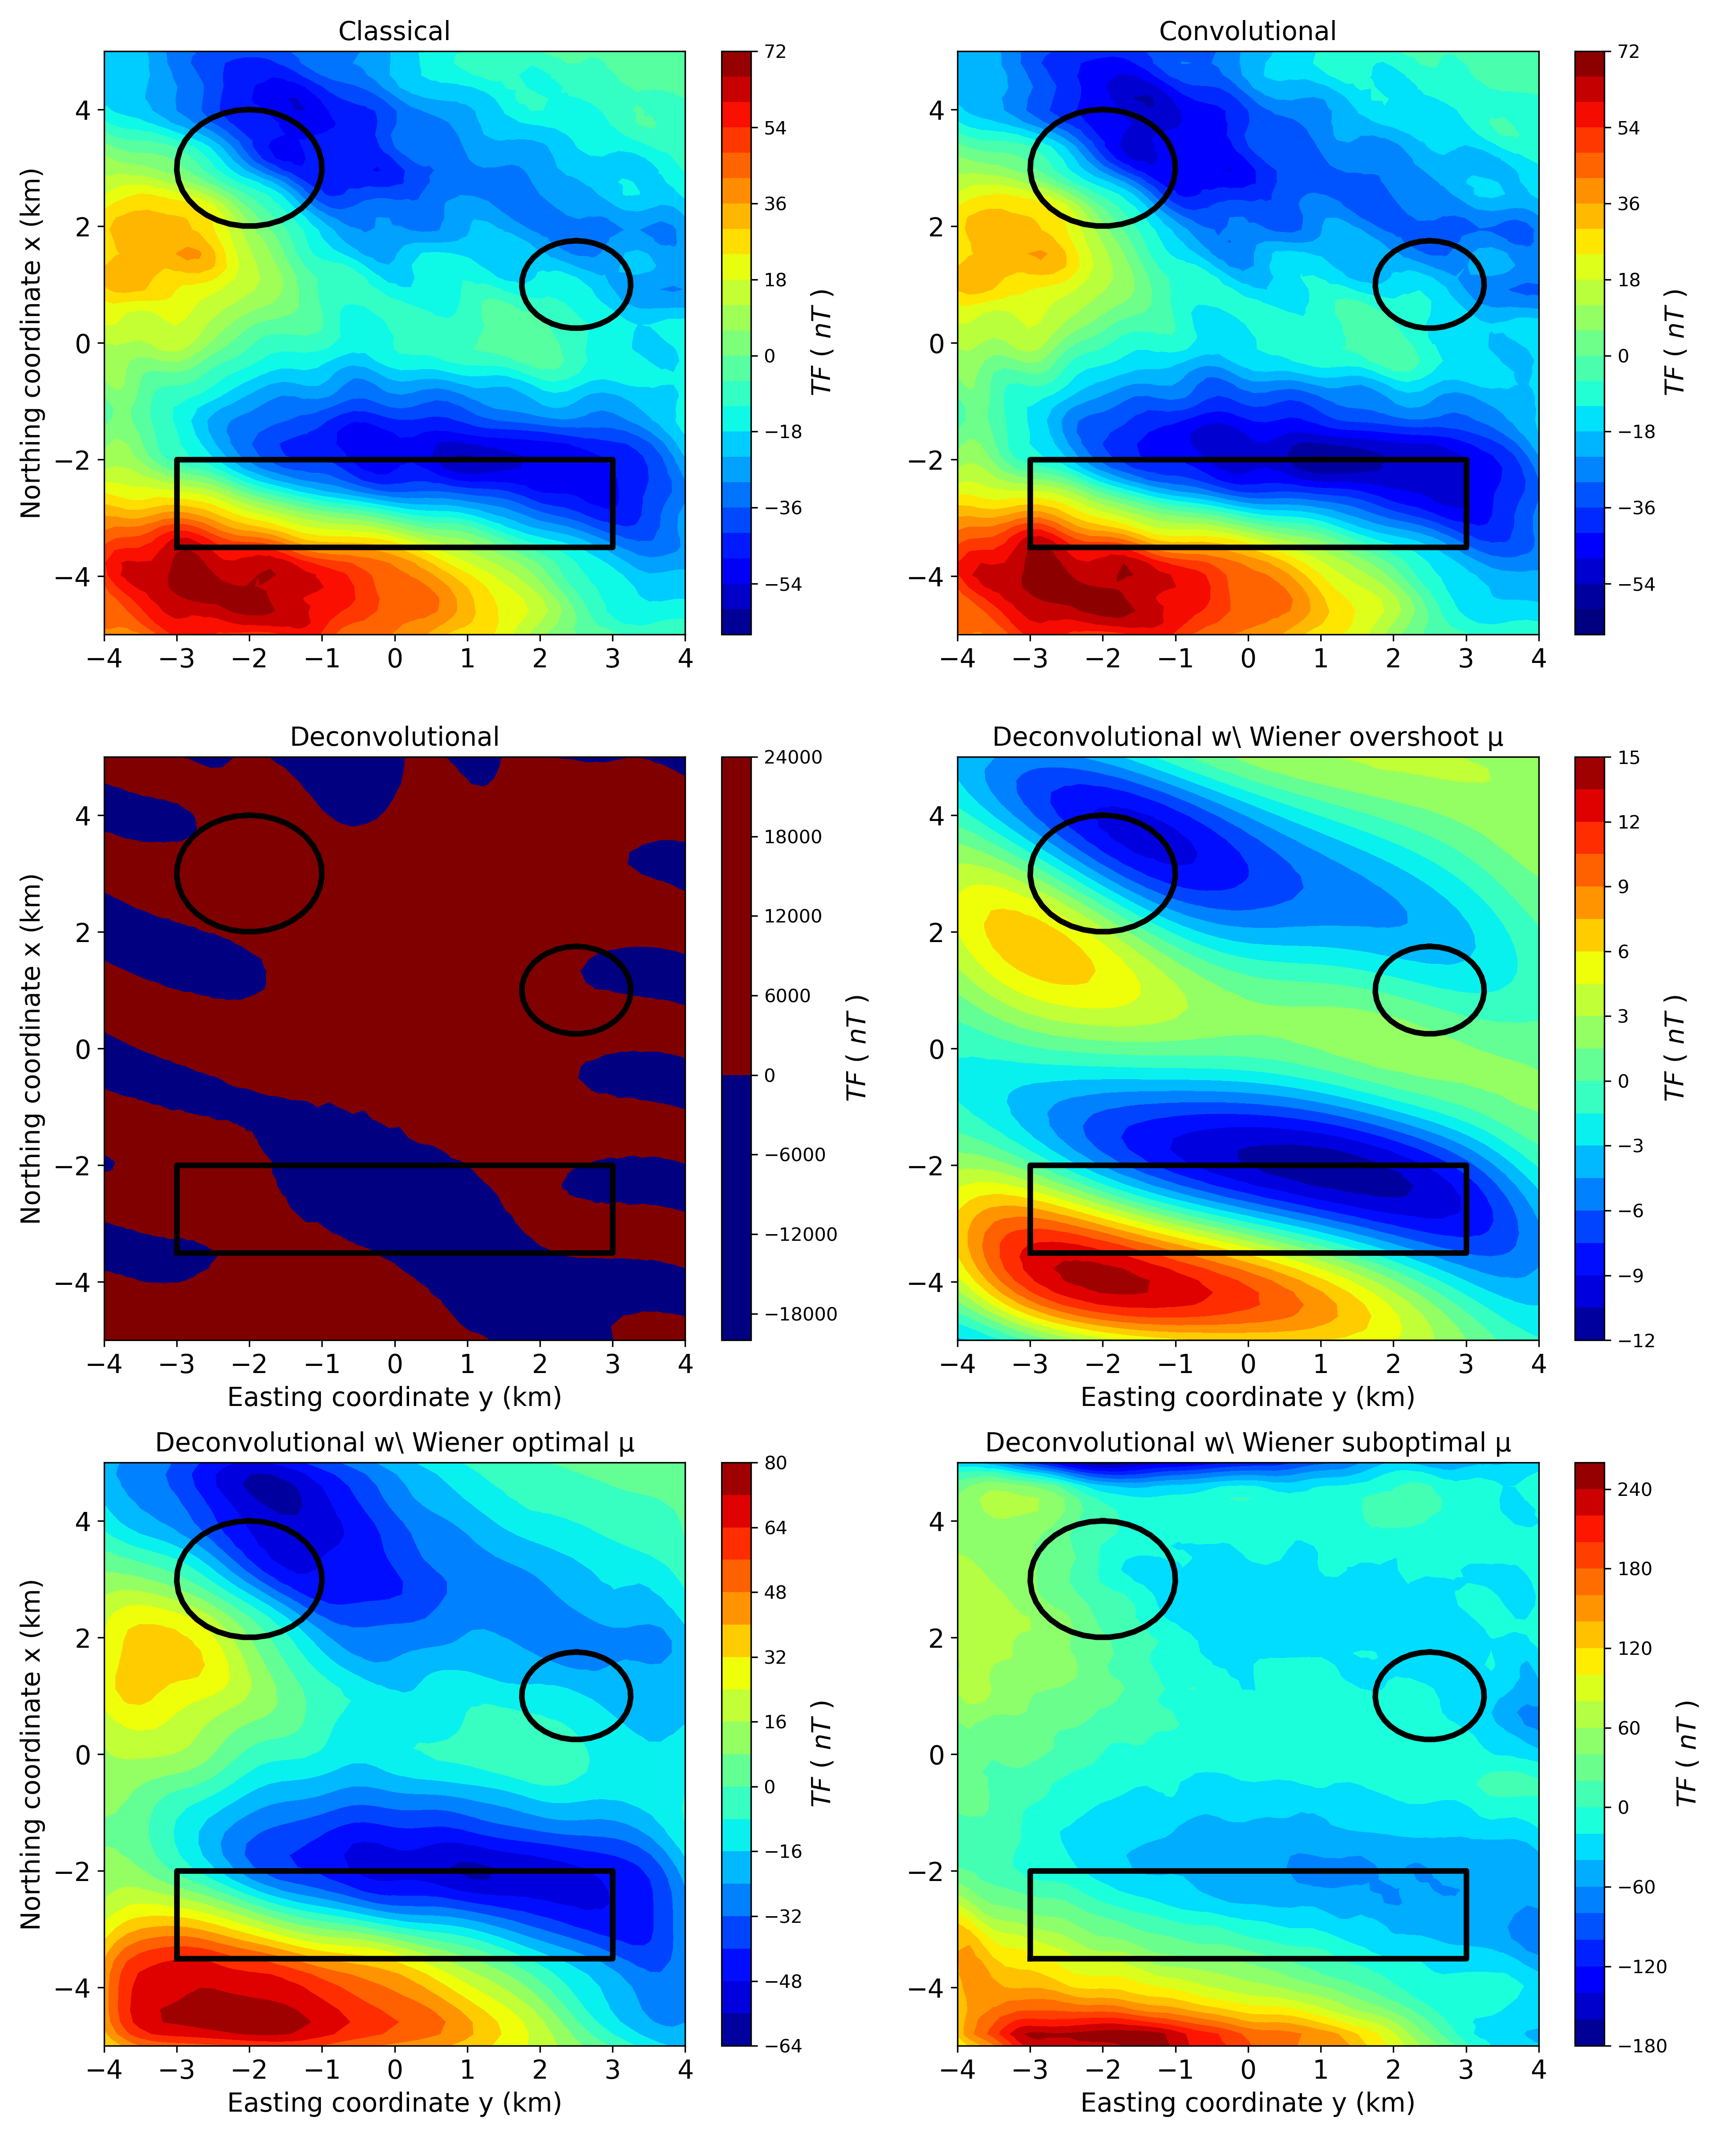
\includegraphics[width=10cm]{Fig/stability_mag_comparison}
	\end{center}
	\caption{Predicted magnetic data for different methods of the equivalent layer with maximum level of noise. Panel \textbf{(A)} is the classical method, \textbf{(B)} is the convolutional, \textbf{(C)} is the deconvolutional, \textbf{(D)} is the deconvolutional method using Wiener stabilization with a too high value for $\mu$, \textbf{(E)} is the deconvolutional method using Wiener stabilization with a optimal value for $\mu$ and \textbf{(F)} is the deconvolutional method using Wiener stabilization with a too low value for $\mu$.}
	\label{fig:8}
\end{figure}

\begin{figure}[htbp]
	\begin{center}
		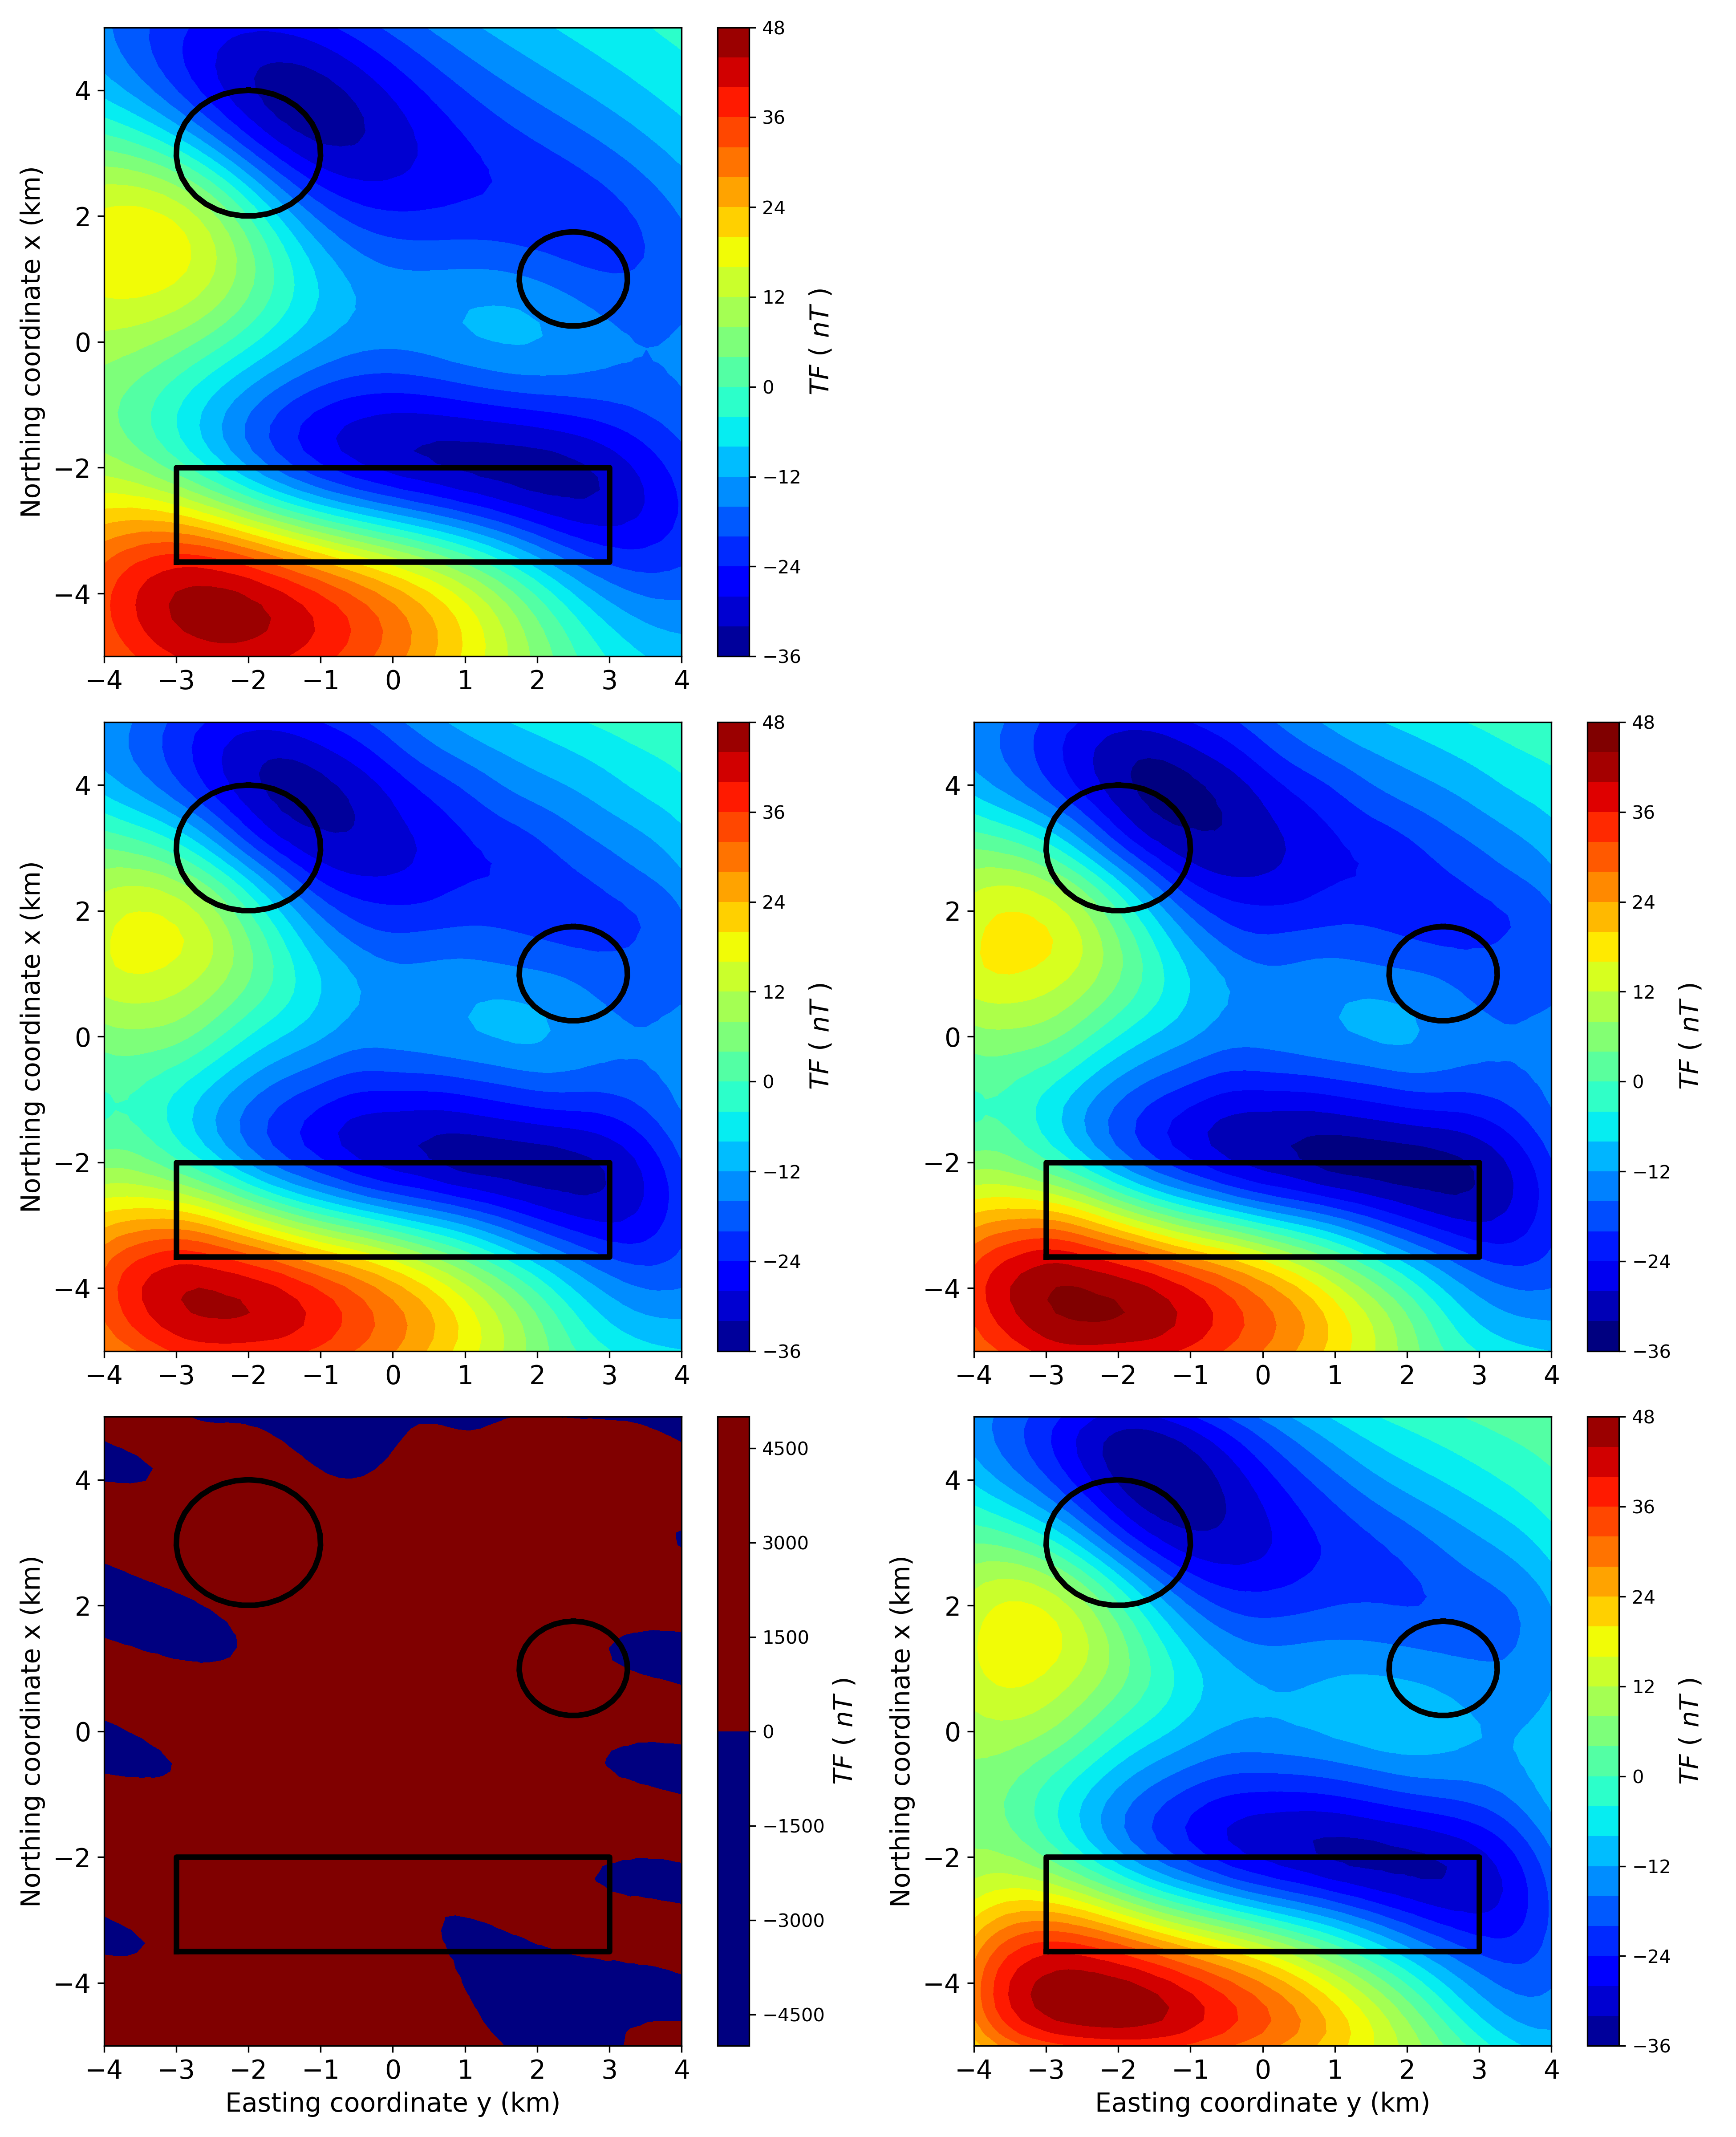
\includegraphics[width=10cm]{Fig/mag_upward}
	\end{center}
	\caption{True noiseless upward magnetic data at $z_i = -1400$ m height and predicted data for different methods of the equivalent layer with maximum level of noise. Panel \textbf{(A)} is the true upward magnetic data, Panel \textbf{(B)} is the classical method, \textbf{(C)} is the convolutional, \textbf{(D)} is the deconvolutional, \textbf{(E)} is the deconvolutional method using Wiener stabilization with a optimal value for $\mu = 10^{-13}$.}
	\label{fig:mag_up}
\end{figure}

\begin{figure}[htbp]
	\begin{center}
		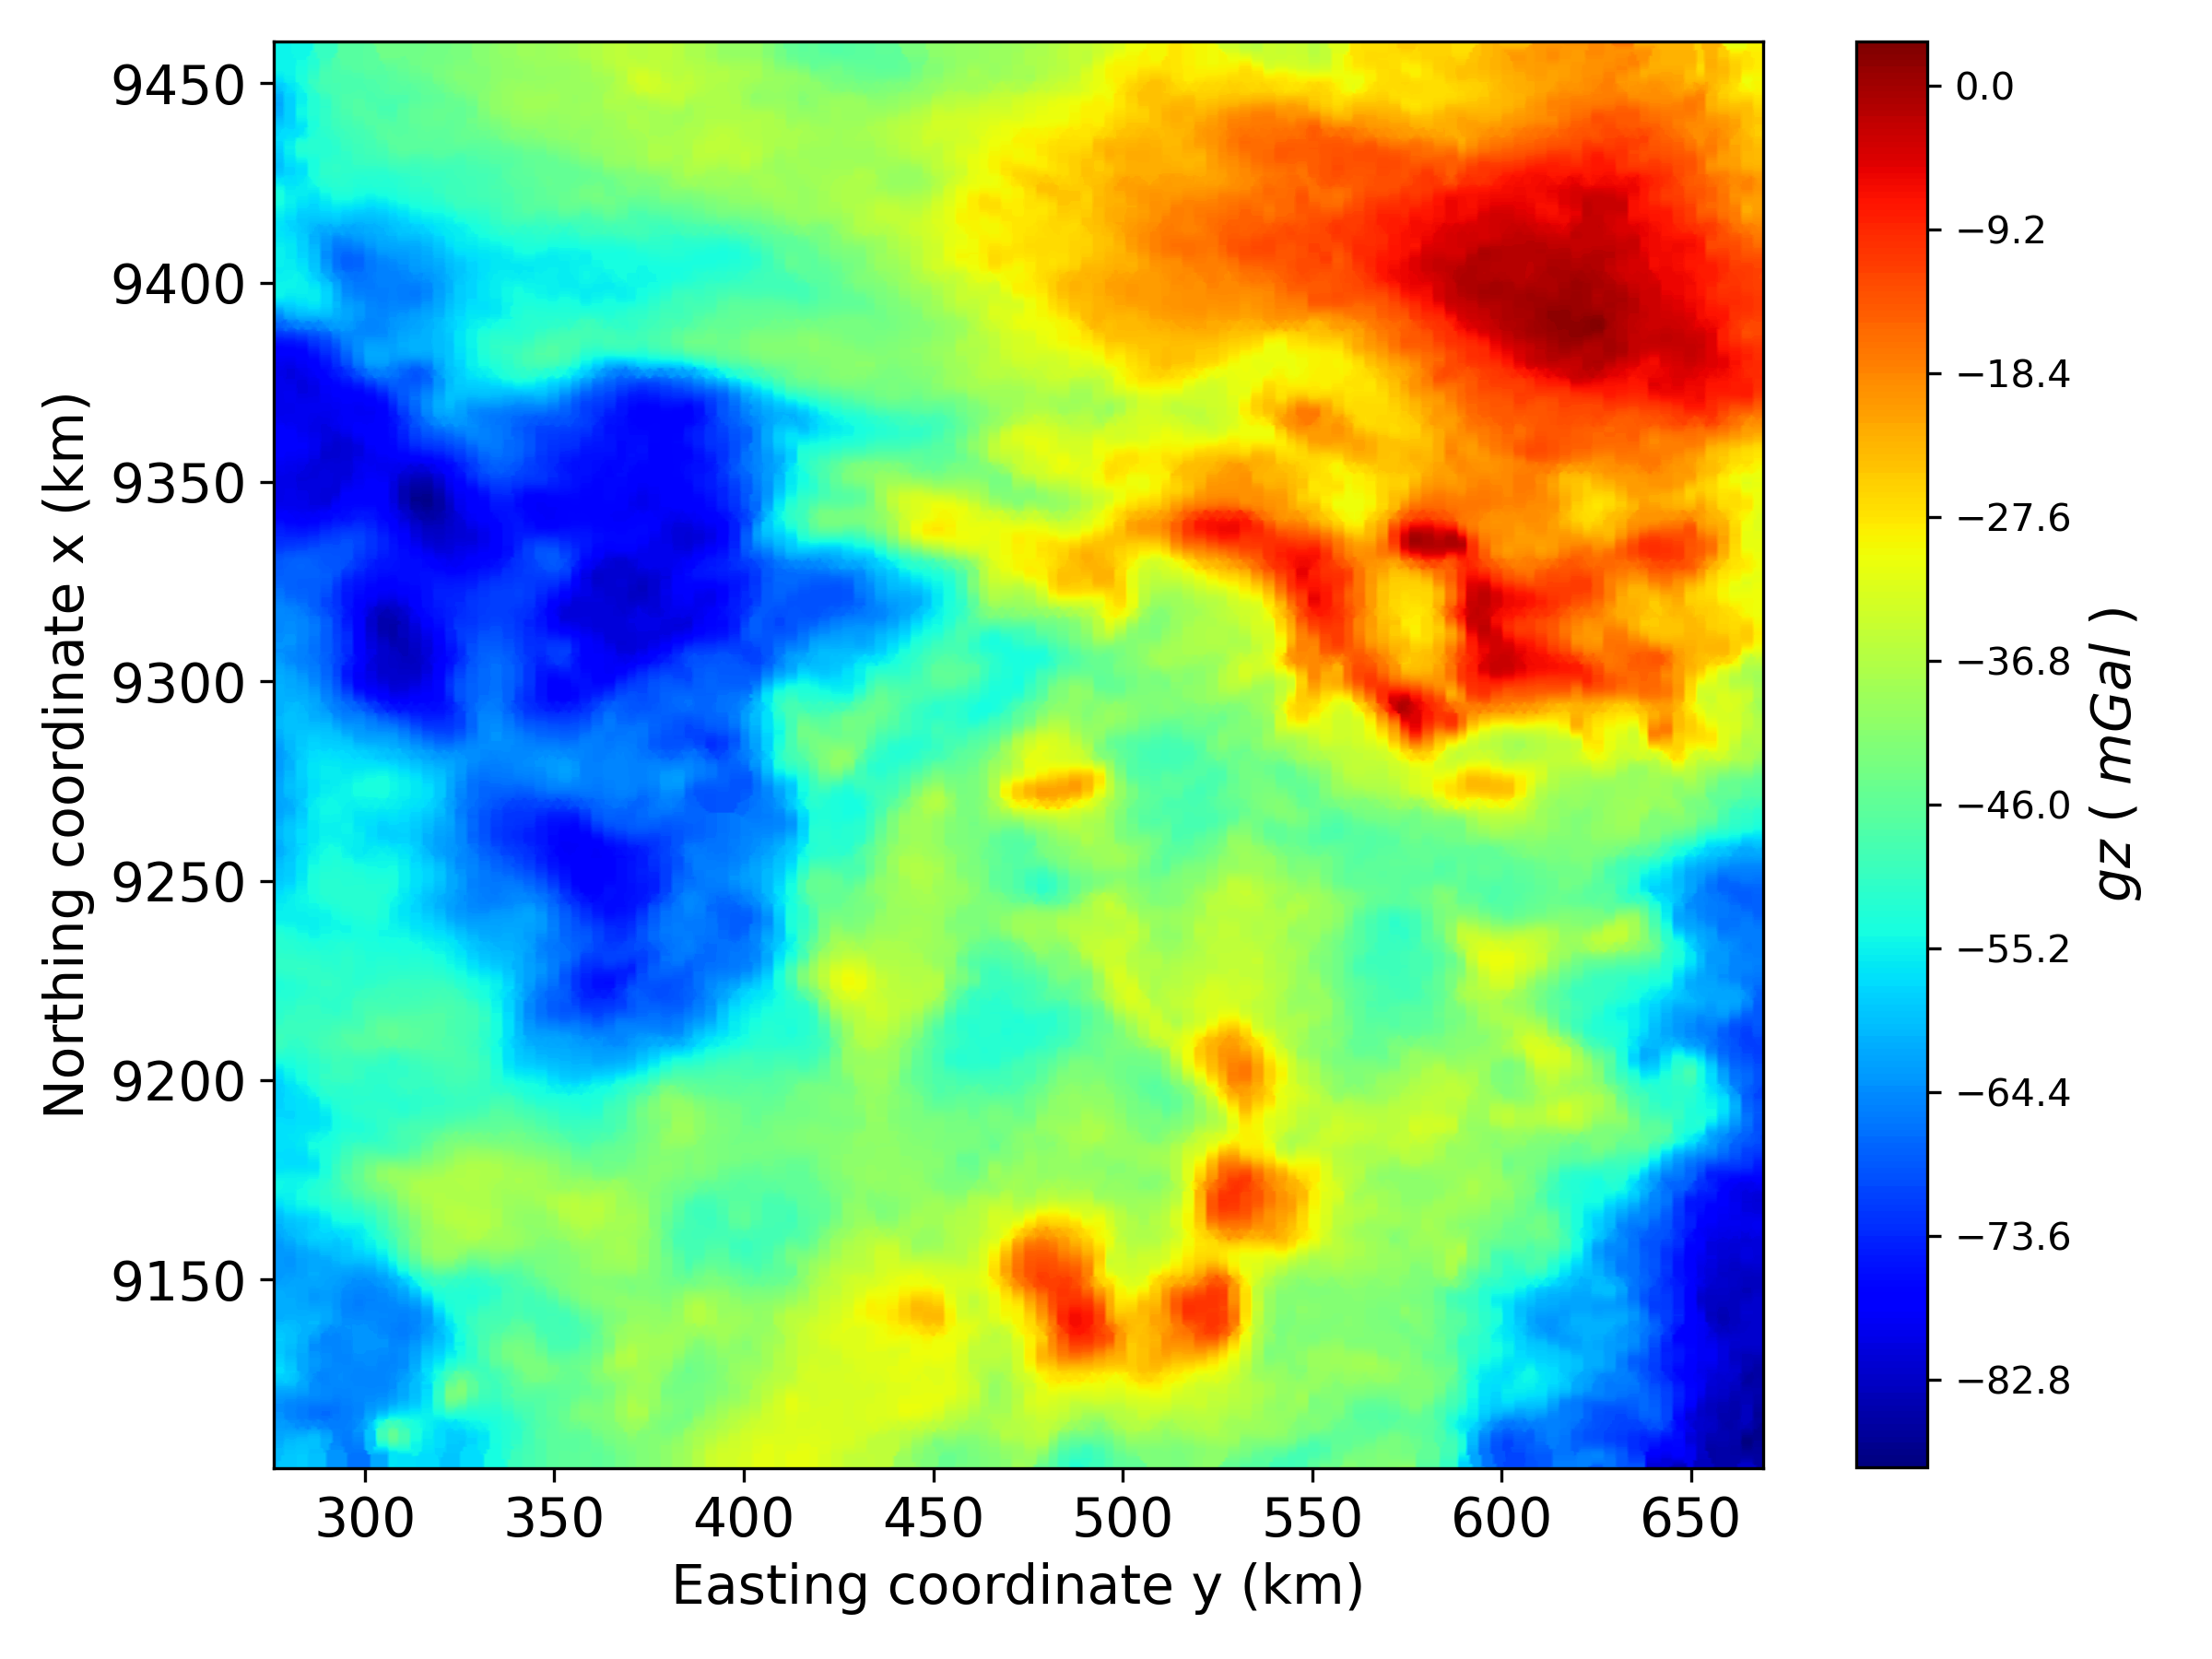
\includegraphics[width=10cm]{Fig/carajas_gz_real_data_1000x500}
	\end{center}
	\caption{Gridded real aerogravimetric data from Carajás, Brazil. A regular grid of $1,000 \times 500$ is being used, totalizing $N,M = 500, 000$ obsevation points and equivalent sources.}
	\label{fig:9}
\end{figure}

\begin{figure}[htbp]
	\begin{center}
		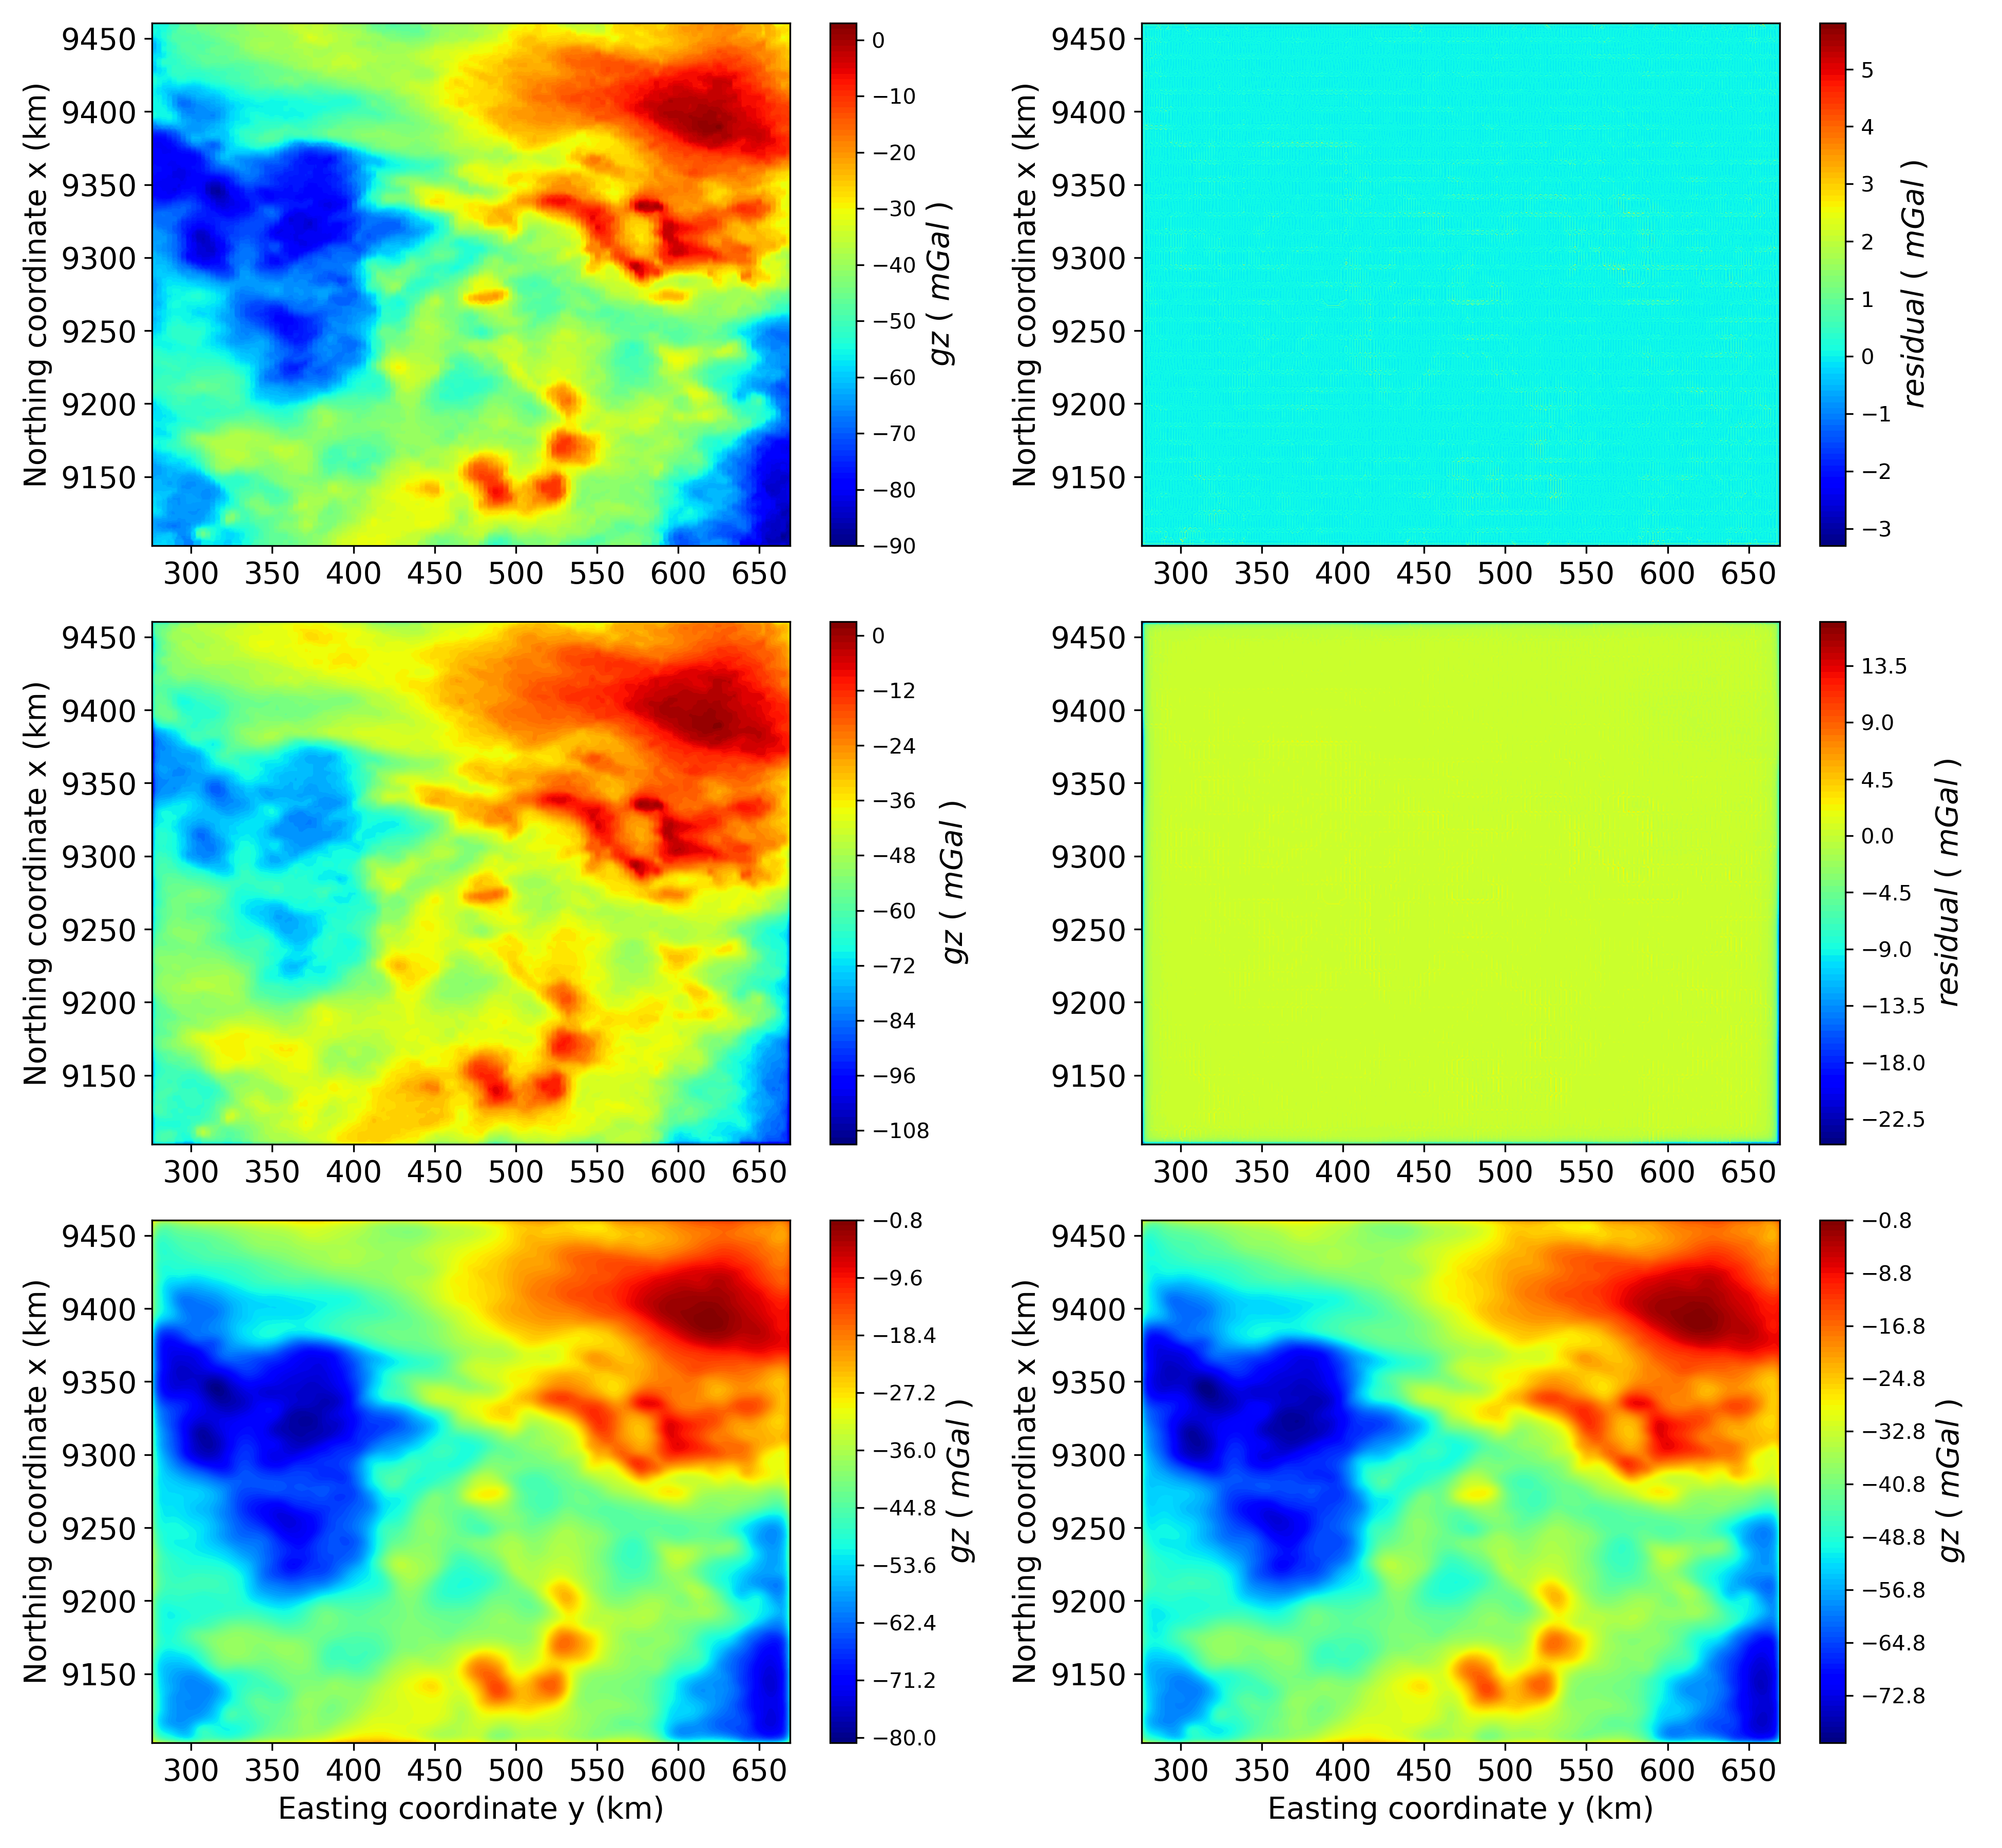
\includegraphics[width=10cm]{Fig/carajas_gz_predito_1000x500}
	\end{center}
	\caption{Panel \textbf{(A)} shows the Carajás predicted gravimetric data from convolutional equivalent layer method. Panel \textbf{(B)} shows the residual from the convolutional equivalent layer method. Panel \textbf{(C)} shows the predicted data from deconvolutional equivalent layer method. Panel \textbf{(D)} shows the residual from the deconvolutional equivalent layer method. Panel \textbf{(E)} shows the upward continuation at $z_i = -3500$ m for the convolutional method and Panel \textbf{(F)} shows the upward continuation at $z_i = -3500$ m for the deconvolutional method.}
	\label{fig:10}
\end{figure}

\begin{figure}[htbp]
	\begin{center}
		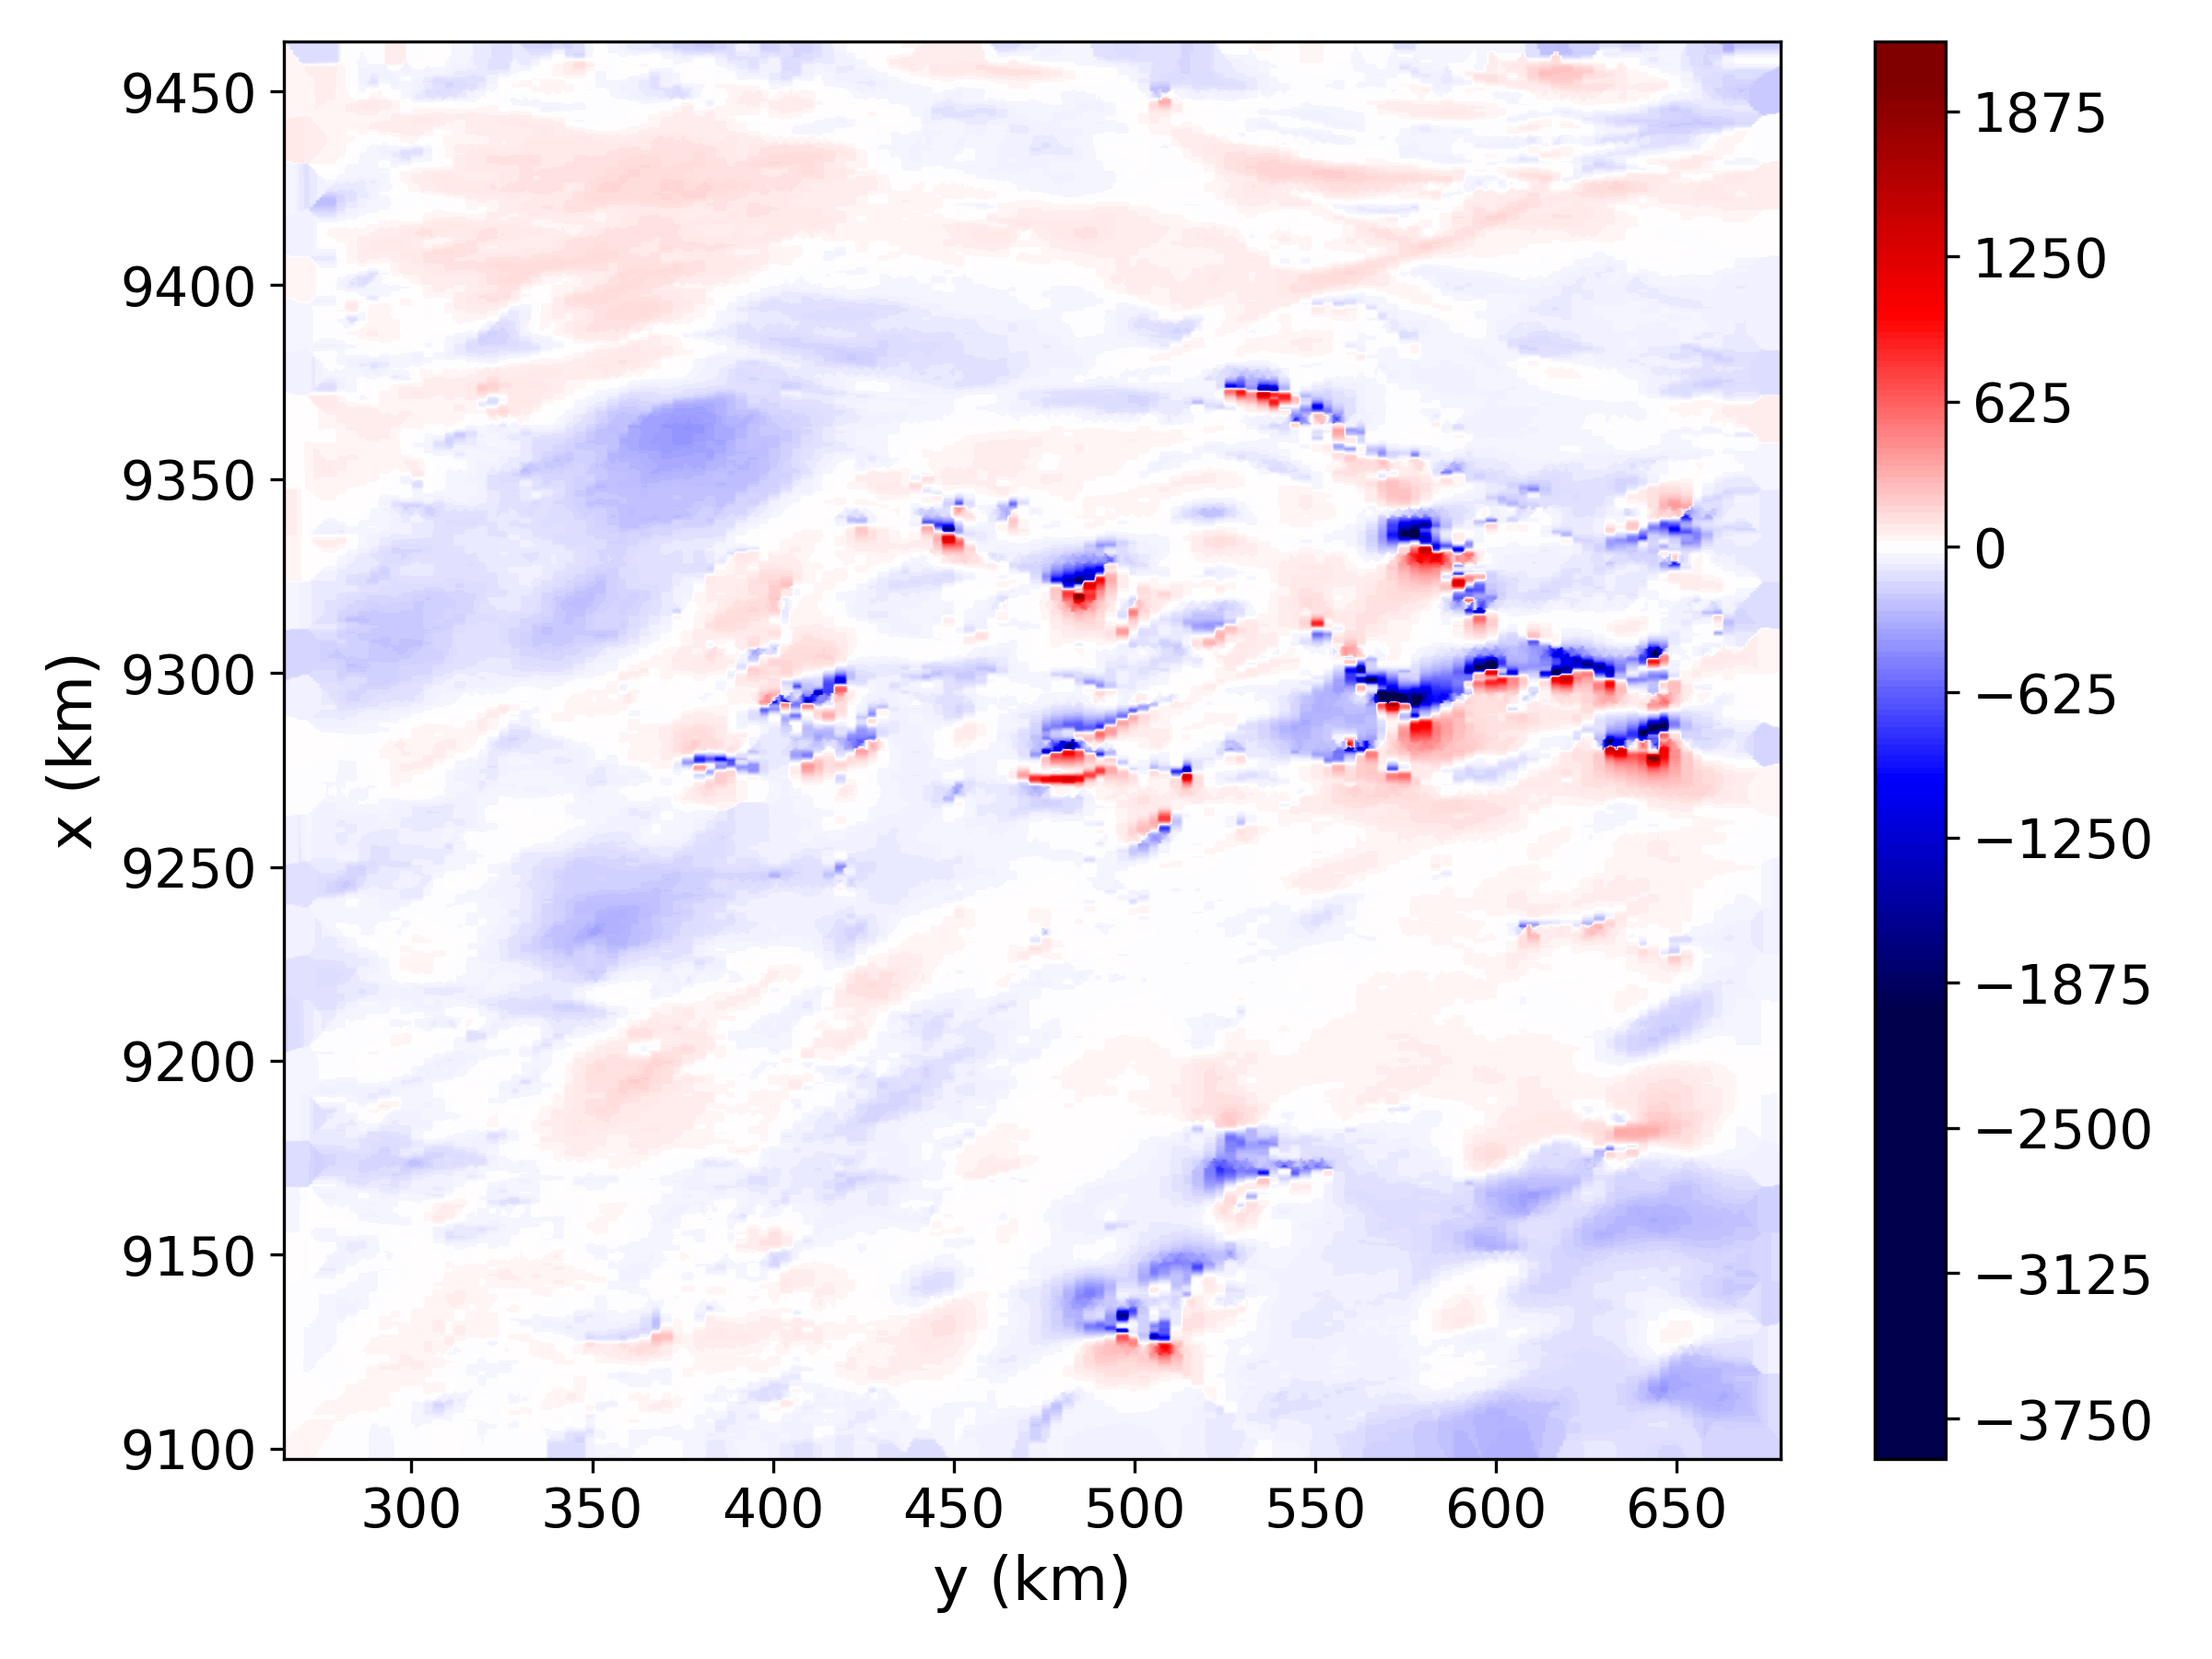
\includegraphics[width=10cm]{Fig/carajas_tf_real_data_1000x500}
	\end{center}
	\caption{Gridded real aeromagnetic data from Carajás, Brazil. A regular grid of $1,000 \times 500$ is being used, totalizing $N,M = 500, 000$ obsevation points and equivalent sources.}
	\label{fig:11}
\end{figure}

\begin{figure}[htbp]
	\begin{center}
		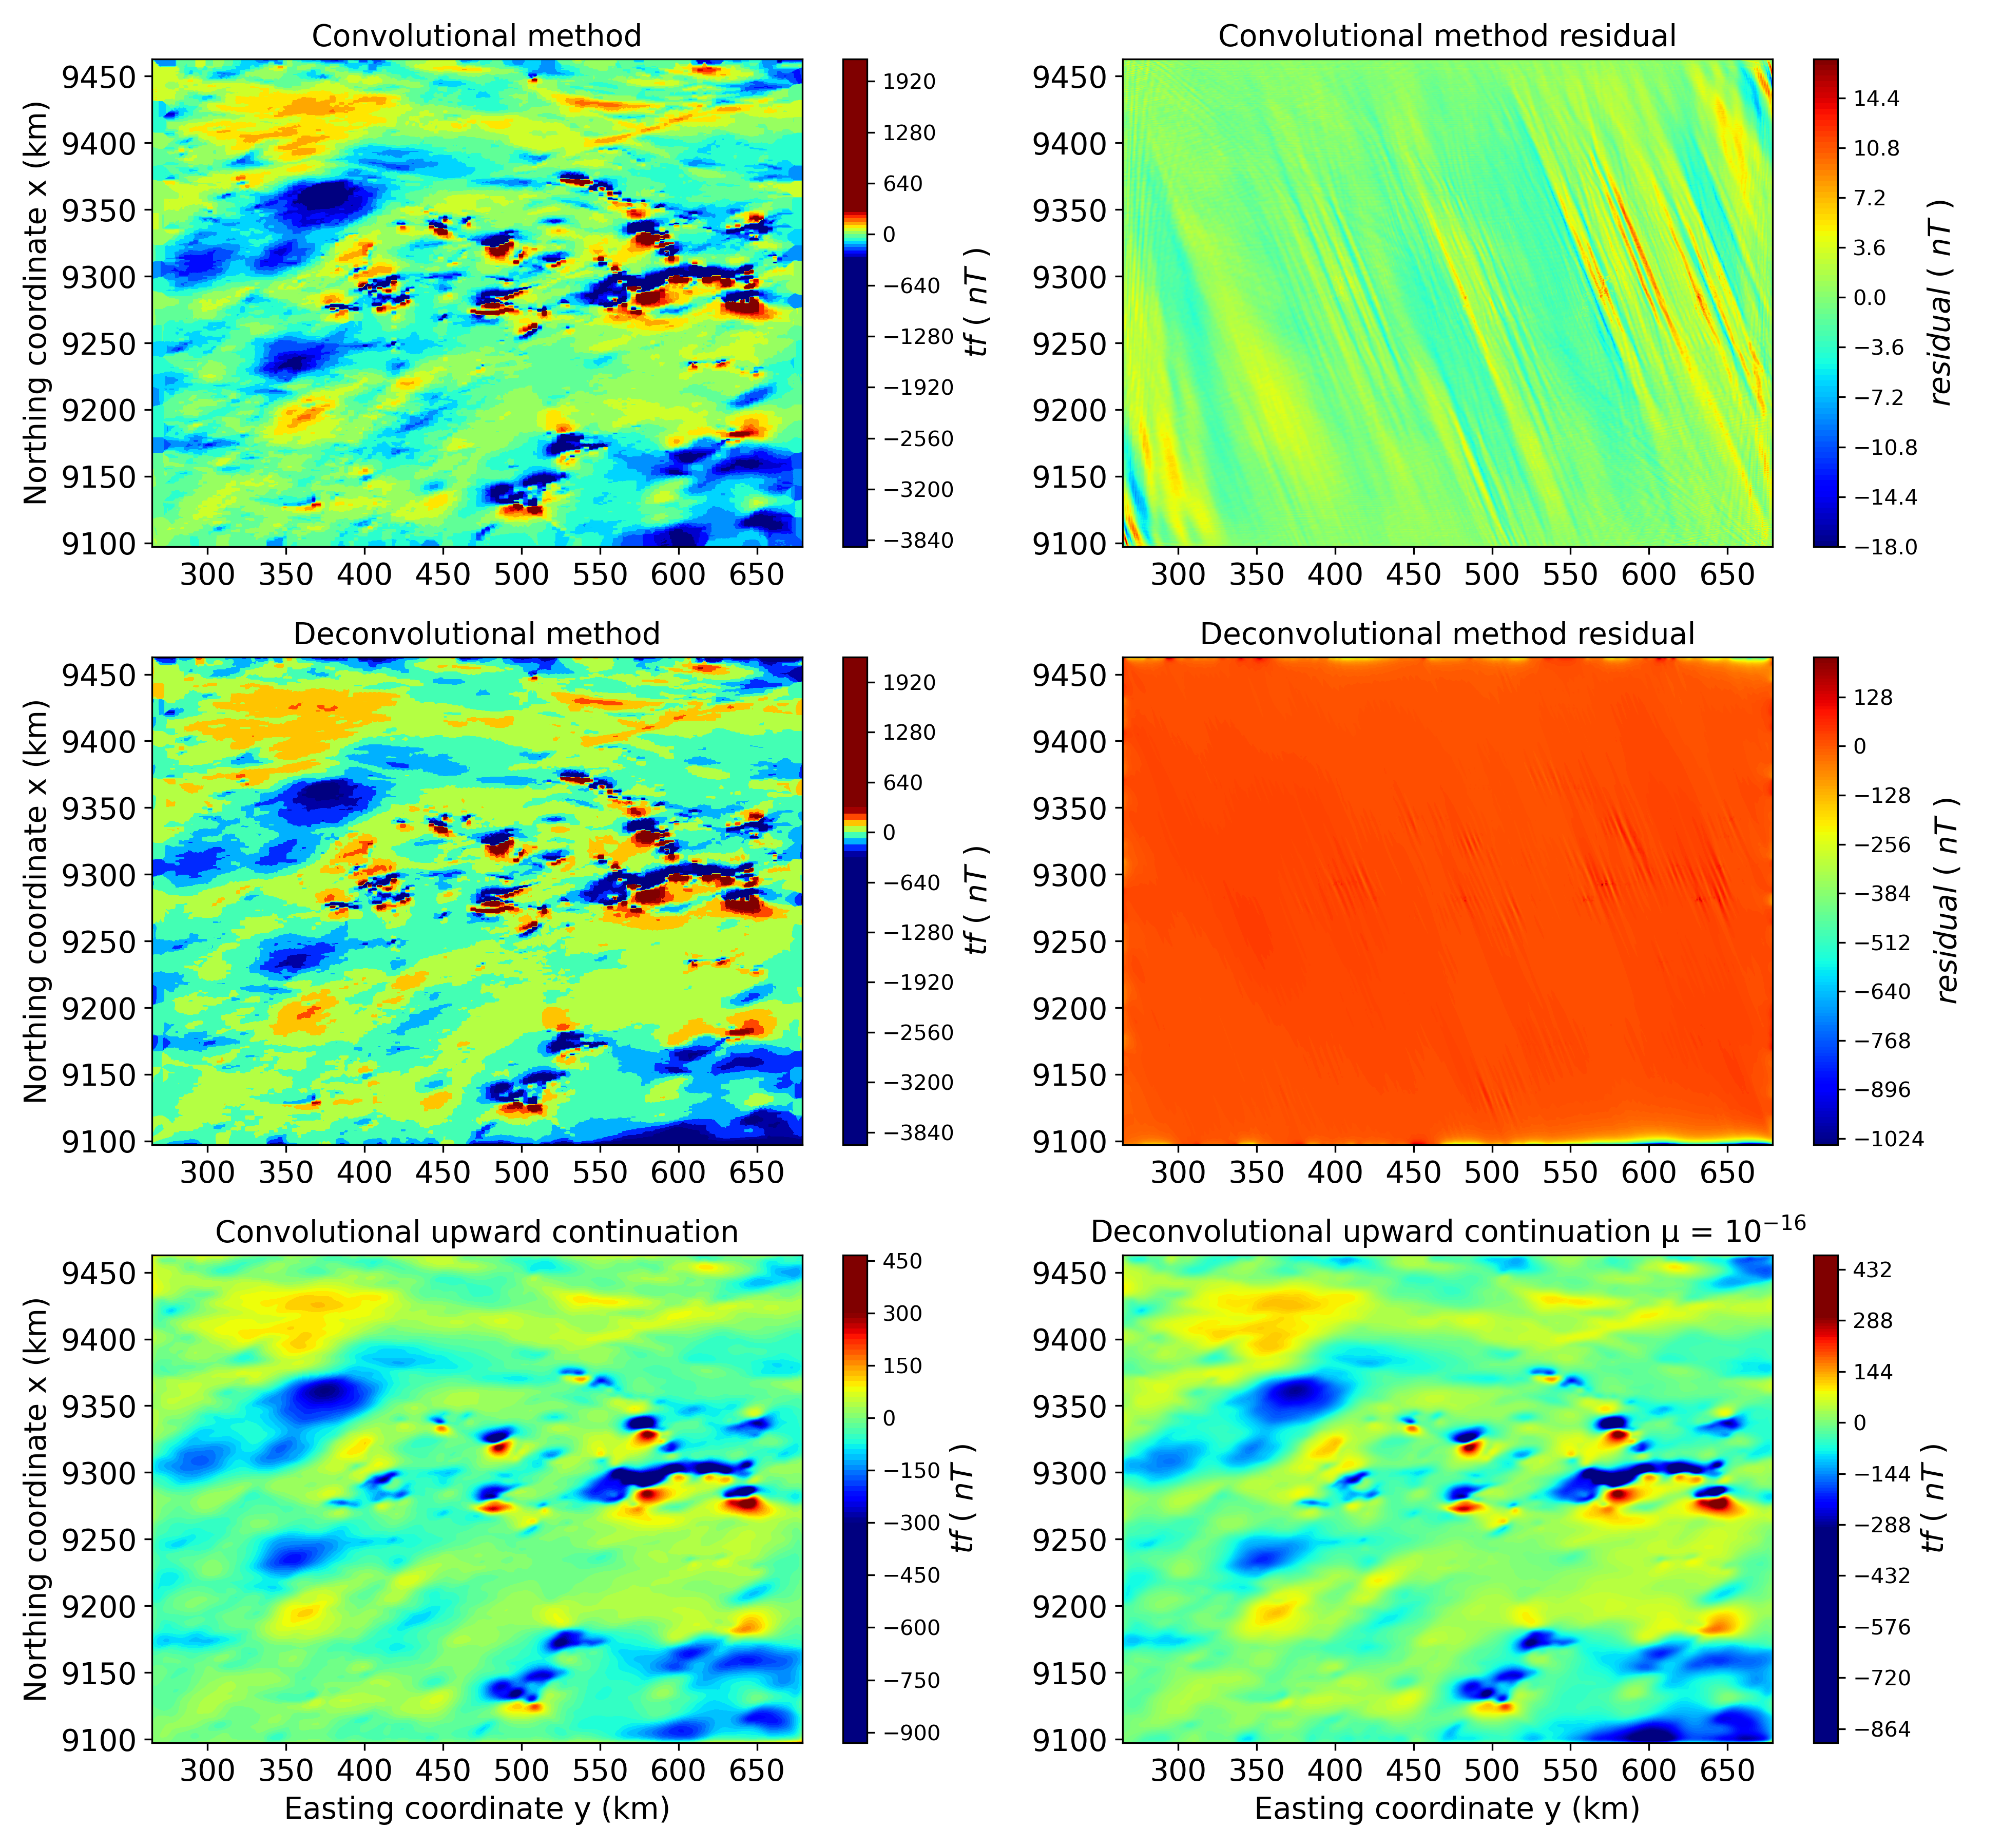
\includegraphics[width=10cm]{Fig/carajas_tf_predito_1000x500}
	\end{center}
	\caption{Panel \textbf{(A)} shows the Carajás predicted magnetic data from convolutional equivalent layer method. Panel \textbf{(B)} shows the residual from the convolutional equivalent layer method. Panel \textbf{(C)} shows the predicted data from deconvolutional equivalent layer method. Panel \textbf{(D)} shows the residual from the deconvolutional equivalent layer method. Panel \textbf{(E)} shows the upward continuation at $z_i = -3500$ m for the convolutional method and Panel \textbf{(F)} shows the upward continuation at $z_i = -3500$ m for the deconvolutional method.}
	\label{fig:12}
\end{figure}

%%% If you are submitting a figure with subfigures please combine these into one image file with part labels integrated.
%%% If you don't add the figures in the LaTeX files, please upload them when submitting the article.
%%% Frontiers will add the figures at the end of the provisional pdf automatically
%%% The use of LaTeX coding to draw Diagrams/Figures/Structures should be avoided. They should be external callouts including graphics.


%\bibliographystyle{frontiersinSCNS_ENG_HUMS} %  for Science, Engineering and Humanities and Social Sciences articles, for Humanities and Social Sciences articles please include page numbers in the in-text citations
%\bibliographystyle{frontiersinHLTH&FPHY} % for Health and Physics articles
%\bibliography{test}

\end{document}


%%% Make sure to upload the bib file along with the tex file and PDF
%%% Please see the test.bib file for some examples of references


%%% RULES FOR FIGURES


%\section*{Figure captions}
%
%%%% Please be aware that for original research articles we only permit a combined number of 15 figures and tables, one figure with multiple subfigures will count as only one figure.
%%%% Use this if adding the figures directly in the mansucript, if so, please remember to also upload the files when submitting your article
%%%% There is no need for adding the file termination, as long as you indicate where the file is saved. In the examples below the files (logo1.eps and logos.eps) are in the Frontiers LaTeX folder
%%%% If using *.tif files convert them to .jpg or .png
%%%%  NB logo1.eps is required in the path in order to correctly compile front page header %%%
%
%\begin{figure}[h!]
%\begin{center}
%
\includegraphics[width=10cm]{logo1}% This is a *.eps file
%\end{center}
%\caption{ Enter the caption for your figure here.  Repeat as  necessary for each of your figures}\label{fig:1}
%\end{figure}
%
%\setcounter{figure}{2}
%\setcounter{subfigure}{0}
%\begin{subfigure}
%\setcounter{figure}{2}
%\setcounter{subfigure}{0}
%    \centering
%    \begin{minipage}[b]{0.5\textwidth}
%        
\includegraphics[width=\linewidth]{logo1.eps}
%        \caption{This is Subfigure 1.}
%        \label{fig:Subfigure 1}
%    \end{minipage}  
%   
%\setcounter{figure}{2}
%\setcounter{subfigure}{1}
%    \begin{minipage}[b]{0.5\textwidth}
%        
\includegraphics[width=\linewidth]{logo2.eps}
%        \caption{This is Subfigure 2.}
%        \label{fig:Subfigure 2}
%    \end{minipage}
%
%\setcounter{figure}{2}
%\setcounter{subfigure}{-1}
%    \caption{Enter the caption for your subfigure here. \textbf{(A)} This is the caption for Subfigure 1. \textbf{(B)} This is the caption for Subfigure 2.}
%    \label{fig: subfigures}
%\end{subfigure}

%%% If you don't add the figures in the LaTeX files, please upload them when submitting the article.
%%% Frontiers will add the figures at the end of the provisional pdf automatically
%%% The use of LaTeX coding to draw Diagrams/Figures/Structures should be avoided. They should be external callouts including graphics.

\end{document}
